% !TeX spellcheck = en_GB
       \documentclass[12pt,pdftex,letterpaper]{article}
%            \usepackage{setspace}
            \usepackage[dvips,]{graphicx} %draft option suppresses graphics dvi display
%            \usepackage{lscape}
%            \usepackage{latexsym}
%            \usepackage{endnotes}
%            \usepackage{epsfig}
            \usepackage{amsmath}
%           \singlespace
            \setlength{\textwidth}{6.5in}
            \setlength{\textheight}{9in}
            \addtolength{\topmargin}{-\topmargin} 
            \setlength{\oddsidemargin}{0in}
            \setlength{\evensidemargin}{0in}
            \addtolength{\headsep}{-\headsep}
            \addtolength{\topskip}{-\topskip}
            \addtolength{\headheight}{-\headheight}
            \setcounter{secnumdepth}{2}
%            \renewcommand{\thesection}{\arabic{section}}
            % \renewcommand{\footnote}{\endnote}
            \newcommand{\Prob}{\operatorname{Prob}}
            \clubpenalty 5000
            \widowpenalty 5000
            \renewcommand{\baselinestretch}{1.50}
            \usepackage{amsmath}
            \usepackage{amsthm}
            \usepackage{amsfonts}
            \usepackage{amssymb}
            \usepackage{cancel}
            \usepackage{bbm}
            \usepackage{graphicx}
            \usepackage{subcaption}
            \usepackage{multirow}
            \usepackage{natbib}
            \usepackage{longtable}
            \usepackage{enumerate}
            \usepackage{setspace}
	\usepackage{rotating}
	\DeclareMathOperator*{\argmax}{argmax}
	\DeclareMathOperator*{\argmin}{argmin}
	\newcommand{\erf}{\text{erf}}
	\newcommand{\Var}{\text{Var}}
	\newcommand{\Cov}{\text{Cov}}
	\newcommand{\pd}[2]{\frac{\partial#1}{\partial#2}}
	\newcommand{\der}[2]{\frac{\text{d}#1}{\text{d}#2}}
	\newcommand{\E}{\mathbb{E}}
	\newcommand{\N}{\mathbb{N}}
	\newcommand{\R}{\mathbb{R}}
	\newcommand{\Type}{\iota}
	\newcommand{\Health}{h}
	\newcommand{\PostHealth}{H}
	\newcommand{\HealthOb}{\Health^*}
	\newcommand{\Excellent}{\Health^E}
	\newcommand{\VeryGood}{\Health^V}
	\newcommand{\Good}{\Health^G}
	\newcommand{\Fair}{\Health^F}
	\newcommand{\Poor}{\Health^P}
	\newcommand{\Utility}{\text{U}}
	\newcommand{\Value}{\text{V}}
	\newcommand{\PostValue}{W}
	\newcommand{\Inc}{I}
	\newcommand{\Con}{c}
	\newcommand{\TotalMed}{M}
	\newcommand{\Care}{m}
	\newcommand{\Invst}{n}
	\newcommand{\Xpend}{X}
	\newcommand{\InvstFunc}{\textbf{\Invst}}
	\newcommand{\ConFunc}{\textbf{\Con}}
	\newcommand{\MedFunc}{\textbf{\Med}}
	\newcommand{\XpendFunc}{\textbf{\Xpend}}
	\newcommand{\MedShkParam}{\gamma}
	\newcommand{\MedShkParamAlt}{\gimel}
	\newcommand{\Bank}{b}
	\newcommand{\Assets}{a}
	\newcommand{\Rfree}{R}
	\newcommand{\DiscFac}{\beta}
	\newcommand{\Premium}{p}
	\newcommand{\Copay}{q}
	\newcommand{\OOP}{o}
	\newcommand{\Subsidy}{S}
	\newcommand{\PremiumFunc}{\text{\Premium}}
	\newcommand{\CopayFunc}{\text{\Copay}}
	\newcommand{\ConFloor}{\underbar{\Con}}
	\newcommand{\LifeUtility}{\varsigma}
	\newcommand{\CRRAcon}{\rho}
	\newcommand{\CRRAcare}{\nu}
	\newcommand{\Age}{j}
	\newcommand{\MaxAge}{J}
	\newcommand{\HealthParam}{\delta}
	\newcommand{\HealthParamAlt}{\daleth}
	\newcommand{\Sex}{s}
	\newcommand{\MedShk}{\eta}
	\newcommand{\HealthShk}{\epsilon}
	\newcommand{\MortParam}{\theta}
	\newcommand{\DiePrb}{\mathsf{D}}
	\newcommand{\LivPrb}{\cancel{\DiePrb}}
	\newcommand{\BequestParam}{\omega}
	\newcommand{\HealthProdFunc}{\text{f}}
	\newcommand{\HealthProdParam}{\kappa}
	\newcommand{\HealthProdParamAlt}{\lambda}
           \newcommand{\BudgetCorr}{\Gamma}
	\newcommand{\State}{x}
	\newcommand{\Control}{y}
	\newcommand{\PostState}{z}
	\newcommand{\Normal}{\mathcal{N}}
	\newcommand{\Indicator}{\mathbf{1}}

\begin{document}

\begin{singlespace}
\title{Optimal Health Investment:\\An Ounce of Prevention at Half Price?}

\author{Matthew N. White$^\dagger$}

\date{\today}

\maketitle

\begin{abstract}
This paper considers how changes in the subsidization of preventive care through public insurance for seniors would affect life expectancy, medical expenses, and government spending.  I augment a standard dynamic consumption-savings model with two medical care goods, ``health investment'' and ``medical consumption'', to create an intertemporal tradeoff in medical care: the former improves the stock of health, reducing the distribution of need for the latter in the future.  I estimate the structural model using data on single, retired Americans from the Health and Retirement Study, matching profiles of health, wealth, and medical spending conditional on several observables.  I then conduct policy counterfactuals to ascertain the effects of alternative subsidy schemes for health investment.  Although there is no policy that universally improves longevity while reducing medical costs (or government spending), I find that decreasing the coinsurance rate for health investment for low and middle income retirees while increasing it for rich retirees would more efficiently allocate health investment to improve longevity \textit{on average} without increasing costs.  Moreover, such a policy would be relatively more generous in its subsidization of health investment for the healthier, younger, and female beneficiaries.
\end{abstract}

\end{singlespace}

\textbf{JEL Classification:} D14, D91, I13

\vspace{0.5cm}

\textbf{Keywords:} \textit{Dynamic optimization, health investment}

\vspace{1cm}
\begin{singlespace}
\noindent \textbf{Notes:} Many thanks are owed to H\"{u}lya Eraslan and Chris Carroll for their feedback during the development of this work, as well as anonymous referees at the Review of Economic Dynamics.  Helpful comments were also provided by Robert Moffitt, Elena Krasnokutskaya, and Nicholas Papageorge.  This study makes use of data from the Health and Retirement Study (HRS); the HRS is sponsored by the National Institute on Aging (grant number NIA U01AG009740) and is conducted by the University of Michigan.

\vspace{1cm}

\small
\noindent $\dagger$ Univ of Delaware, Dept of Economics (416B Purnell Hall, Newark DE 19716);  mnwecon@udel.edu
\end{singlespace}

\thispagestyle{empty}
\newpage

\section{Introduction}
\label{sec:Intro}

It is well established that wealthier individuals live longer and have better health (\cite{deaton02}); and conditional on current health, richer individuals experience slower health deterioration (\cite{case03}) and spend more on medical care.  It is likewise uncontroversial that, all else equal, healthier people have lower medical expenses (\cite{thorpe04}).  These facts suggest an intuitive story: Those with more resources are better able to invest in their health through medical care, leading to lower future health expenditures than they would have in the absence of this investment.  If the decision of how much health investment to purchase is driven by budgetary concerns, lowering its out-of-pocket cost could motivate lower income individuals to better preserve their health.  They would thus need less medical care to manage disease in the future, potentially resulting in a net decrease in total demand for medical services.  The Patient Protection and Affordable Care Act includes such subsidies, significantly increasing the generosity of Medicare's coverage for preventive care.  President Obama asserted that this provision ``provid[es seniors] the kind of preventive care that will ultimately save money throughout the system.''\footnote{First Presidential debate, October 3, 2012.  Obama has made similar claims on other occasions.}

Is it possible for the government to \textit{save} money or reduce total medical expenditures by more generously subsidizing health investment for seniors?  More generally, how much should the government subsidize health investment through public insurance in order to most efficiently improve health and extend life?\footnote{\cite{ellis07} theoretically demonstrate that the efficient level of insurance coverage for preventive care is positive; here I consider whether public insurance meets or exceeds the efficient level.}  The answers to these questions depend on several margins, including the extent to which health investment produces health capital; the relationship among health status, longevity, and medical expenses; and how individuals value their health relative to other goods.

An economic model suitable for analyzing these questions must incorporate each of these margins to capture a key intertemporal tradeoff between medical care in the present and future: Additional purchases of preventive care improve the distribution of health in the population, which in turn reduces the need for care to mitigate or cure future ailments.  Existing models treat medical spending either as an investment in the stock of health (as in the classic \cite{grossman72} model) or as a stochastic shock to wealth (e.g.\ \cite{dinardi10}), but these models must be combined to address the dynamic effects of a subsidy on health investments.

To do so, I specify and estimate a structural model of the ``retirement life cycle'' that incorporates the key features of both lines of prior models.  My model includes two medical care goods: ``health investment'' (representing both preventive and curative medical care), which affects the subsequent stock of health; and ``medical consumption'' (representing care to mitigate or manage pain, disability, or symptoms from medical conditions), the need for which depends stochastically on health.  This two-good structure creates the intertemporal tradeoff in medical care purchases, and is thus suitable for evaluating a counterfactual subsidy on health investment.  This model is one of the first to employ a two-good approach\footnote{Previous models with two medical care goods specify both as consumption goods, as in \cite{blau08}, or both as investment goods, as in \cite{ozkan14}.} to medical expenses to address both the consumption and investment aspects, and thus combine the two major strands of the literature.

The direct approach to estimating the effects of a subsidy on preventive care would be to find a source of exogenous variation in the cost of care across individuals and examine the differential results.  In the absence of such observed variation, this paper takes an indirect approach by structurally estimating preference and health production parameters consistent with observed differential health outcomes by \textit{income and wealth}.  That is, individuals with different levels of wealth and permanent income will make different health investment choices that lead to disparate health outcomes; the estimation ``backs out'' the extent to which individuals can improve future outcomes through health investment and how much they value health and longevity (relative to consumption) by matching observed conditional outcomes with those from the simulated model.

Specifically, I use the simulated method of moments on data from the Health and Retirement Study (HRS) to match conditional profiles of assets, medical expenses,\footnote{I do not separately observe health investment and medical consumption in the HRS data, but rather their sum as simply medical care.  The estimation procedure endogenously separates the two medical care goods as it fits medical expense and health transitions across income and wealth groups.} health, and mortality.  I then simulate the effects of counterfactual public insurance policies that provide alternate cost sharing schemes for health investment and compare the outcomes to a baseline simulation.  In this way, variation in one element of the intertemporal optimization problem (current financial resources and expectations of future resources) is used to indirectly ascertain the effects of varying another element of the problem (the out-of-pocket unit cost of health investment). 

I find that it is \textit{not} possible to reduce total medical expenses (nor government spending) by decreasing cost sharing for health investment beyond what is provided by baseline Medicare.  The subsidy policy that would minimize total medical expenses is universally less generous than the baseline policy (but not necessarily zero), so further increasing subsidies for health investment would also increase costs.  If they had to pay full price for investment, retirees in the bottom three income quintiles would purchase less than the level that would minimize their total expected medical costs, because a large fraction of those costs are paid by Medicare (and other insurance); providing \textit{some} subsidy for health investment thus reduces total lifetime medical expenses.  In contrast, rich individuals paying full price for health investment would purchase more than the total-cost-minimizing quantity, as their very high valuation of additional periods of life more than offsets the effect of the cost externality.  The total-medical-expense-minimizing subsidy policy thus offers essentially \textit{no} insurance for health investment for the top two income quintiles.

Likewise, there is essentially no alternative policy that increases life expectancy for any group while decreasing government expenditures on that group.  However, the model predicts that it is possible to increase longevity \textit{on average} without increasing government spending by (in effect) redistributing health investment from the top income quintile to the bottom three income quintiles.  That is, increasing cost sharing for the richest retirees significantly decreases their purchases of health investment (and thus government spending on them) with relatively small effects on health and longevity.  The savings can then be used to more generously subsidize health investment for lower income retirees, who incur higher medical expenses through greater investment (in total and for the government), but generate larger increases in health and life expectancy. The ``socially optimal'' subsidy policy thus tries to align individual retirees' incentives with choosing the efficient level of health investment.  The model likewise reveals that a subsidy scheme that induces retirees to choose an efficient level of investment is relatively more generous towards younger, healthier, and female beneficiaries for whom additional health produces more years of life expectancy than their older, sicker, and male peers.

My model does not capture all features relevant to the determination of total demand for medical care in response to a change in the subsidization of health investment.  A more complete model would account for multi-person households, as in husband-and-wife bargaining models (e.g.\ \cite{blau06}), to address the sharing of resources and joint optimization.  Moreover, the model ignores the role of other health-related behaviors-- such as drinking, smoking, and exercise-- considered by others in the literature (e.g.\ \cite{khwaja10}).  The choice of insurance contract is not modeled (as in \cite{cardon01} and \cite{einav13}), but instead exogenously assigned based on observable characteristics using reduced form estimates.  While prior work has provided strong evidence that medical expenses exhibit a significant degree of serial correlation (see e.g.\ \cite{french04}), my model assumes medical need shocks that are iid; other features of the model generate \textit{some} serial correlation, the extent seen in the data is not replicated (see Figure \ref{fig:SerialCorrOOP}).  Finally, the identifying assumptions make the approach taken here suitable for analyzing only the retired population, for whom income risk is low and (critically) does not depend on health.  This restriction also limits the applicability of the findings to the population on which the model was estimated; usage, efficacy, and willingness to pay for health investment by the working age population might be significantly different.


\subsection{Discussion}
\label{sec:Disc}

The model employs two medical care goods-- ``medical consumption'' and ``health investment''.  Medical consumption represents \textit{mitigative care}, which is used to relieve or manage pain, disability, or symptoms associated with an illness (e.g.\ morphine). It contributes to the patient's current utility but does not improve future health.  Health investment represents both \textit{curative care} and \textit{preventive care}. The former is employed to treat the illness itself and thus avert future pain, disability, or symptoms (e.g.\ penicillin); the latter is used to prevent an illness from arising or progressing in the first place (e.g. the flu vaccine).  They both act like an investment good by influencing the underlying health stock: preventing degradation in good health (preventive care) or increasing the stock in bad health (curative care).

A model individual's ``medical needs'' are randomly drawn each period, determining how much medical consumption is valued relative to consumption of other goods and services.  Because the distribution of medical needs depends on the health state, current health investment reduces future medical consumption-- the critical intertemporal tradeoff.  The model thus includes both transitory shocks (via current medical needs) and permanent shocks (to the health stock, driving medical needs in all future periods) to medical spending, with agents endogenously affecting the permanent shocks through their health investment decision.

When individuals purchase health investment, they are essentially trading wealth for health; the rate at which they can make this tradeoff depends on the slope of the health production function.  Under the standard logic of tangency between preferences and constraints, they are willing to invest up to the point where the ``marginal health product'' of a dollar spent out of pocket on health investment equals the ratio of their marginal values of wealth and health.  The familiar envelope condition from many consumption-saving models holds in this setting, so the marginal value of wealth equals (discounted) expected marginal utility of future consumption.\footnote{My model includes a bequest motive, so the marginal value of wealth also includes expected marginal ``warm glow'' utility from bequeathing one's estate.}  Agents in the model value health for several reasons, but the counterfactual analysis reveals that the primary factor is their valuation of additional longevity; this is primarily determined by the expected future \textit{level} of utility relative to being dead.  With any risk averse utility function, richer individuals' higher expected consumption means they have a lower marginal value of wealth (through lower marginal utility of consumption) and a higher marginal value of health (due to higher expected levels of utility each period); assuming decreasing returns to health from health investment, they will thus purchase \textit{more} investment than poorer individuals.

Longevity is not the sole motivation for retirees to invest in their health, as a greater level of health capital also brings lower medical needs (in distribution).  This both \textit{directly} improves utility through smaller shocks and \textit{indirectly} by reducing expenses for medical care to mitigate the utility loss, freeing up resources for future consumption.  However, a substantial portion of these medical expenses are covered by Medicare, and I estimate that public insurance is more generous for sicker retirees-- the coinsurance rate is \textit{increasing} in health status (see Section \ref{sec:Constructions}).  Likewise, Medicare also subsidizes health investment (before any expansion through the ACA), so seniors do not pay full price for investment.

Agents in the model thus \textit{do not fully internalize} the benefits (nor costs) of health investment, as they are insured against high medical expenses and the extent of their insurance decreases slightly with improved health.  Further, individuals in the model are protected against extremely adverse shocks through a consumption floor, representing Medicaid and other means tested programs.  As the poorest retirees are the most likely to require assistance from the consumption floor, and are the least willing to trade wealth for health, they are the most likely candidates to underutilize health investment, leaving on the table significant potential health gains that would incur a relatively small cost to produce.  Conversely, the richest retirees highly value additional life; Medicare's existing subsidization of health investment thus might induce them to purchase at an inefficiently high level, yielding little additional health while creating significant medical costs.  In Section \ref{sec:SocOpt}, I consider how the government \textit{should} subsidize health investment (by income, health, and age) if it is willing to incur a particular cost per year of life added (in total medical expenses), efficiently choosing the public insurance policy.

The key parameters of the model that determine how simulated individuals react to alternative policies are identified by matching health transitions as they vary by income and assets. Conditional on current health, wealthier individuals have better future health outcomes.  My model explains these differential patterns through endogenous variation in the level of health investment purchased: Wealthier individuals have lower marginal value of wealth and higher marginal value of health, making them more willing to trade wealth for health to attain more periods of life, consistent with \cite{hall07}.  As in \cite{arcidiacono07}, zero health investment by poorer individuals can be optimal if their expected utility in subsequent periods is not sufficient to justify sacrificing consumption for the sake of additional health.  The efficacy of the investment good in producing health (in both slope and curvature) and direct utility of living are identified by variation in the rate of health decline across income quintiles.\footnote{A complete discussion of identification can be found in Section \ref{sec:Ident}.}

While the restriction of the estimation sample to older, retired individuals limits the applicability of the analysis, it is also \textit{necessary} in order to employ this identification strategy.  In the classic \cite{grossman72} model, health capital allows workers to be more productive and/or to supply more labor, increasing their income.\footnote{For an overview of the empirical literature supporting this prediction, see \cite{currie99}.}  The causal relationship between health and income thus runs both ways for individuals during their working life, so that identifying the parameters of the health production function via differences in the rate of health decline by income is impossible.  For the retired population, in constrast, the flow of income is exogenous of health status.

By explaining variation in the rate of health decline across income and asset levels solely through different levels of health investment, my model takes a strong stand on a phenomenon that could have other origins.  For example, wealthier individuals could have a higher discount factor, which earlier in life motivated them to invest in human capital to generate their high income and now causes them to forgo unhealthy behaviors, extending their lives.  Alternatively, the income-rich might be more efficient producers of health, able to generate better outcomes from the same dollar value of medical inputs through more informed selection of services. Even without unobserved heterogeneity, there are non-medical channels through which wealthier individuals could make health investments, including diet, exercise, and alcohol and tobacco (non-)usage.  Moreover, the causality could be reversed: unhealthy individuals frequently missed work, preventing productivity growth and keeping their incomes low.  Related, the nature of low-paying jobs might have affected workers so that health is not only lower but also deteriorates faster.

Each of these effects' exclusion makes the estimation and simulation more likely to find that more generously subsidizing health investment could reduce total medical expenses.  That is, adding any of these elements to the model would provide an additional channel for explaining differential health profiles, attenuating the estimated efficacy of health investment and/or willingness to pay for it.  This strengthens the result that decreasing cost sharing on health investment could not be cost-saving, with each simplifying assumption biasing the estimation to find the opposite.  The estimates presented here should thus be interpreted as an upper bound on the benefits of such a policy.\footnote{Alternatively, the implied cost per added year of life should be interpreted as a lower bound.}



\subsection{Literature}
\label{sec:Lit}

My model draws from two lines of literature on medical expenses, each of which are insufficient on their own to capture the intertemporal tradeoff between health investment and medical consumption.  Literature that treats medical spending as an investment in a stock of ``health capital'' allows health to be endogenous to individuals' decisions, but ties all medical spending directly to the magnitude of the (permanent) health shock; these models can thus only match the large observed variance of medical expenses with a very large variance of permanent health shocks that is not seen in the data.  On the other hand, literature that considers the role of medical expenses in motivating saving by the elderly can match the extreme variance of medical spending, but treats health as exogenous and thus cannot endogenously explain differences in health outcomes across income levels.  When these models are combined, health investment in the present can be used to shift down the distribution of other medical expenses in the future.

Economic models of health investment can be traced back to Grossman's 1972 model in which agents' optimal stock of health declines as they age due to the rising costs of maintaining health.  In recent work, \cite{yogo09} models health as a continuous variable that evolves according to normally distributed shocks, conditional on current health and log medical spending.  While the model is used to explain differences in mean medical spending by health and other covariates, his model does not address the large variance of medical spending within any given group.  In his model, all variation in medical expenses is driven by shocks to the health state (whose variance is calibrated from the data), so the simulated variance of expenses is likely much too small.

\cite{ozkan14} uses a model with two medical care goods to explain the profiles of medical spending by wealthy and poor individuals, specifying both medical care goods as investments in two stocks of health capital.  Physical capital determines survival probabilities, while preventive capital governs the distribution of shocks to physical capital; neither type of care can improve the stock, merely offset potential current period losses from health shocks-- the health stocks are monotonically decreasing over time.\footnote{In both the HRS and the Medical Expenditure Panel Survey (MEPS) data used by Ozkan, neither individuals' subjective categorization of health nor objective health measures (e.g.\ individual conditions) are monotonically decreasing; rather, health state transitions can be positive or negative.}  Critically, any forgone medical care (below the maximum productive level that period) results in a permanent, unrecoverable loss of health; medical expenses are thus directly linked to the distribution of permanent health shocks.   The health capital stocks in the Ozkan model are unobservable abstractions, so the estimation does not attempt to match rates of health decline, only longevity and medical expenses.  In contrast, my estimation treats health as an observable quantity and decouples permanent \textit{health} shocks from transitory \textit{medical need} shocks so that it can match both (stochastic, non-monotonic) health deterioration rates across wealth and income and the distribution of medical spending by health.

Other recent structural models of health investment employ a binary health state and discrete investment decision.  \cite{papageorge16} models HIV positive men as they make decisions about treatment and labor supply; taking retroviral drugs reduces the likelihood that the HIV infection will develop to AIDS (and increases the probability of regaining a high CD4 white blood cell count after the onset of AIDS), but generates side effects that both directly reduce utility (through discomfort) and increase the disutility of working.  The agent's future wages depend on his work history, so Papageorge's model has a tradeoff (and causality) between \textit{long run} income and health.  \cite{aizawa17} develops an equilibrium labor market model of firms (who decide whether to offer employer sponsored insurance) and workers (who sort into jobs based on the compensation package); the dynamics of the binary health state depend on a binary medical care utilization decision.

My model's closest ancestor is \cite{dinardi10} (hereafter ``DFJ''), which explores how large and volatile medical expenses motivate saving among the elderly.  The model particularly draws from their specification in which the quantity of medical care is determined endogenously rather than as an exogenous shock.  DFJ are able to match asset and medical spending profiles of the very old, and they find that the serial correlation of medical needs shocks is a major motivation for the savings maintained by even wealthy retired individuals.  My model mirrors the structure of DFJ, but adds a second medical care good that affects the health state transition rather than treating income as a direct input into health evolution.  Further, I capture the serial correlation of medical needs shocks through persistence of a continuous health variable, in contrast to DFJ's specification of binary health with underlying permanent shocks to medical needs.

Related models also do not focus on the tradeoff between present medical spending to invest in health and future medical spending to mitigate illness,\footnote{One exception is \cite{yang08}, who consider the long run effects of an expansion of Medicare on both health and fiscal outcomes.  Very recent work by \cite{cronin16} models medical decision-making for each month \textit{within} an insurance coverage year, with endogenously evolving health, allowing for intertemporal shifting of care.} as they treat medical care as a single good or omit savings.  Both \cite{french11} and \cite{blau08} investigate how retiree health insurance benefits--- the ability of a worker to continue to purchase medical insurance from an employer after retirement--- affects the decision to retire before reaching Medicare age.  Blau and Gilleskie model the medical care decisions of men approaching retirement as they make discrete decisions about work and medical care utilization; the medical care goods affect both utility and the health state transition probabilities.  Khwaja (2010) estimates a discrete choice model of consumption, medical expenses, and health-affecting behaviors (smoking, alcohol consumption, exercise) to estimate the willingness to pay for Medicare.  Assets and saving behavior are not modeled, with individuals assumed to consume any remaining income after paying insurance premiums and out-of-pocket medical costs.  While medical care again provides direct utility and affects health evolution, it is modeled as a unitary good.  \cite{depreux11} considers how Medicare can generate an anticipatory or ex ante moral hazard effect on the same health behaviors considered by Khwaja, estimating a reduced form based on a discrete choice model that also does not include a savings decision.  In contrast, my model incorporates individuals' ability to ``self insure'' through savings, building from the canonical work of \cite{carroll97b}.

Recent work by \cite{aizawa15} estimates a general equilibrium model of the labor market in which firms choose compensation packages combining wages and health insurance, and workers select into jobs based on these offers (and their heterogeneous needs).  The general equilibrium structure allows them to match a rich set of outcomes and to credibly simulate variations on ACA-style reforms to the health insurance market.  Because of their focus on employment outcomes rather than precautionary motives and risk aversion, health and medical expenses are exogenous in their model, and saving is not allowed.  Parallel to my restriction of single retired individuals to eliminate the effect of health on income, the authors manage complexity from life cycle concerns and skill heterogeneity by focusing their estimation on early prime-age workers with no more than a high school education.

The medical literature is somewhat pessimistic about the cost efficiency of preventive services.  Near universal application of a preventive service (a screening test, say) will often have costs that outweigh its benefits because the majority of recipients will test negative, offering no medical benefit; moreover, because type II errors are much more costly, these tests will tend to generate many false positives, resulting in further costs. The scientific consensus is that while some universal applications of preventive care (such as childhood vaccinations) reap significant savings, the majority of services studied so far do not (\cite{russell93,russell07,russell09}).  Intuitively, preventive interventions are more cost efficient when more narrowly targeted at the most at risk population, extracting the most expected benefit from each application.  If a wide array of preventive services are subsidized for a population that has low utilization rates, the individuals who receive a service as a result of the subsidy are those who were marginal between its costs and benefits before the subsidy and thus the most efficient group for each treatment.

Preventive care services are generally categorized into \textit{primary} preventive care, which reduces the probability of an illness or condition arising at all, and \textit{secondary} prevention, which detects a condition early to reduce its severity through appropriate treatment (\cite{russell86}).  Most, but not all, forms of preventive care used by seniors are considered to be secondary prevention.  In a JAMA study on underutilization of care by elderly Americans, \cite{asch00} identified forty ``necessary'' medical care indicators, including three they labeled as preventive: visiting a doctor every year, assessing visual impairment every two years, and having a mammogram every two years (for women).  All three necessary preventive measures were found to have lower utilization in high poverty areas.\footnote{This study did not include individual-level income data.}  In an older study of the under-use of preventive care by Medicare recipients, \cite{chao87} consider five types of preventive care: blood pressure test, fecal blood test, Pap smear test, mammography, and breast self-examination.\footnote{The latter is preventive care, but not a \textit{medical} procedure in th usual sense; it does not require any special equipment nor training, and (by definition) can never have an out-of-pocket cost.}  \cite{keyhani07} study usage rates of preventive care among retired male veterans as they vary by public insurance plan, considering influenza vaccination, pneumococcal vaccination, cholesterol testing, and prostate-specific antigen measurement; they find that prevention usage rates do systematically vary among insurers.\footnote{From lowest to highest: Medicare fee-for-service, Medicare HMO plans, Veterans Health Administration.}  In the economics literature, \cite{hsieh97} study the relationship between seniors' health information (specifically, knowing the symptoms of several chronic diseases) and their use of preventive care, focusing on whether an individual has had their blood pressure, blood sugar, or urine (for ketone level) checked in the past year.  Other than the influenza and pneumococcal vaccinations, all of these measures focus on detecting a condition before it develops, so that its impact can be contained by treatment.  The public use HRS has limited data on specific use of some of these preventive services; in Section \ref{sec:Data}, I present reduced form evidence that usage of preventive care is, in fact, increasing in income.

The remainder of the paper proceeds as follows: Section \ref{sec:Model} specifies a dynamic model of consumption and savings with two medical care goods; Section \ref{sec:Data} describes the HRS data and transformations thereof used in the estimation; Section \ref{sec:Est} describes the SMM estimation method and identification strategy and presents parameter estimates and model fit; Section \ref{sec:Counterfactual} conducts counterfactuals of the subsidy on preventive care; and Section \ref{sec:Conc} concludes.



\section{Model}
\label{sec:Model}

In this section, I build a consumption-saving model with two medical goods.  I specify each of the major components in turn-- including the utility function, the distribution of medical needs, and the distribution of the subsequent health state-- before moving on to a description of its solution and a discussion of the modeling choices.

Individuals in the model, indexed by $i$, represent unmarried retired persons over the age of 65 living in the United States.  Individuals are lifetime expected utility maximizers who geometrically discount future utility flows by factor $\DiscFac$ per (two-year) period.  Individual $i$'s state at the time he chooses his controls at time $t$ (when he has reached age $j_{it}$) is given by \textit{b}ank \textit{b}alances $\Bank_{it} \geq 0$, a stock of \textit{h}ealth $\Health_{it} \in [0,1]$, and a medical need shock $\MedShk_{it} > 0$.  The health stock ranges from the worst possible living health state $\Health_{it} = 0$ to ``perfect'' health of 1.  The individual must choose non-negative quantities of three goods: \textit{c}onsumption $\Con_{it}$, \textit{m}edical consumption $\Care_{it}$ (representing mitigative care), and health i\textit{n}vestment $\Invst_{it}$.\footnote{All three goods' prices are normalized to 1, so that spending on each good is equivalent to its quantity.} Bank balances not spent are retained as \textit{a}ssets (\textit{a}fter \textit{a}ll \textit{a}ctions) $\Assets_{it} \geq 0$, which earn interest at risk-free return factor $\Rfree$.

Individuals in the model are \textit{ex ante} heterogeneous: Each $i$ belongs to exactly one of a finite number of \textit{types} indexed by $\iota$.  Each type is characterized by a sex $\Sex_\iota \in \{0,1\} \equiv \{\text{female, male}\}$ and a sequence of non-capital income that is received at each age conditional on survival, $\{\Inc_{\iota j}\}_{j=0}^J$.  In all notation below, a subscript $\iota$ indicates that the object (i.e. variable, function, or distribution) is shared across all individuals of that type, while a subscript $i$ is used when the object varies idiosyncratically within a type.  Further, I will use subscript $\iota j$ to indicate that the object is shared within a type conditional on age, and subscript $it$ for variables whose idiosyncratic value is not determined until period $t$.\footnote{With the obvious exception of $j_{it}$, which is deterministic from the individual's birth cohort.}

\subsection{Model Features}
\label{sec:ModelSpec}

The basic sequence of events for agent $i$ in period $t$ is:
\begin{enumerate}
\item $i$ survives from age $j_{it-1}$ to age $j_{it} = j_{it-1} + 1$ depending on a mortality shock.

\item $i$ learns his health state $\Health_{it}$, conditional on survival.

\item $i$ receives non-capital income $\Inc_{\iota j}$, earns interest on assets $\Assets_{it-1}$, and pays insurance premiums $\Premium_{it}$.

\item $i$ learns his medical need shock $\MedShk_{it}$.

\item $i$ chooses quantities $\Con_{it}$, $\Care_{it}$, and $\Invst_{it}$ subject to his budget constraint.

\item $i$ experiences a flow of utility and returns to his health investment.
\end{enumerate}
I explain these elements below, ordered for ease of exposition rather than chronologically.

\vspace{0.5cm}

\noindent \textbf{Preferences:} The utility flow of a living individual $i$ at time $t$ depends on composite consumption $\Con_{it}$, medical consumption $\Care_{it}$, and the realization of his medical needs shock $\MedShk_{it}$.  I assume all individuals have a common utility function given by:
\begin{equation}\label{Utility}
\Utility(\Con_{it},\Care_{it};\MedShk_{it}) = \frac{\Con_{it}^{1 - \CRRAcon}}{1 - \CRRAcon} + \frac{(\Care_{it}/\MedShk_{it})^{1 - \CRRAcare}}{1 - \CRRAcare} - \frac{\LifeUtility^{1 - \CRRAcon}}{1 - \CRRAcon}, \qquad \CRRAcare > 1. \qquad \LifeUtility > 0.
\end{equation}
Note that nedical consumption is simply a second consumption good with a random marginal utility\footnote{Equivalently, the medical needs shock determines how expensive it is to purchase an ``effective'' unit of mitigative care.} determined by the realization of the medical need shock $\MedShk_{it}$. 

An individual who died at the beginning of period $t$ receives a one time ``warm glow'' utility flow based on the level of assets that he leaves for his heirs, representing his bequest motive.  This ``grave utility'' is given by:
\begin{equation}\label{Bequest}
\grave{\Utility}(\Assets_{it-1}) = \BequestParam_1 \cdot \frac{(\Assets_{it-1} + \BequestParam_0)^{1 - \CRRAcon} - \BequestParam_0^{1 - \CRRAcon}}{1 - \CRRAcon}.
\end{equation}

\vspace{0.5cm}

\noindent \textbf{Medical needs distribution:} The medical needs shock $\MedShk_{it}$ is lognormally distributed; the underlying normal distribution's mean depends on the individual's age $j_{it}$, sex $\Sex_i$, and health $\Health_{it}$, and its standard deviation depends linearly on health status.  Formally:
\begin{equation}\label{MedShkDstn}
\log(\MedShk_{it}) \sim N(\mu_{it}, \sigma_{it}^2), \qquad \mu_{it} = \MedShkParam_0 + \MedShkParam_{\Sex} \Sex_{\iota} + \MedShkParam_{j1} j_{it} + \MedShkParam_{j2} j_{it}^2 + \MedShkParam_{\Health 1} \Health_{it} + \MedShkParam_{\Health 2} \Health_{it}^2, \qquad
\sigma_{it} = \MedShkParam_{\sigma 0} + \MedShkParam_{\sigma 1} \Health_{it}.
\end{equation}
I will collectively refer to the parameters $\MedShkParam$ as the medical shock parameters.

\vspace{0.5cm}

\noindent \textbf{Health depreciation and production:} The individual's health stock evolves as a stochastic function of his age, sex, health, and quantity of health investment $\Invst_{it}$.  The health evolution process proceeds in three three steps.

First, ``end-of-period health'' or ``post-investment health'' is determined based on the current health state and health investment:
\begin{equation}\label{PostHealth}
\PostHealth_{it} = \HealthParam_0 + \HealthParam_{\Sex} \Sex_\iota + \HealthParam_{j1} j_{it} + \HealthParam_{j2} {j_{it}}^2 + \HealthParam_{\Health 1} \Health_{it} + \HealthParam_{\Health 2} \Health_{it}^2 + \HealthProdFunc(\Invst_{it}).
\end{equation}
Additional future health is produced according to health production function $\HealthProdFunc(\Invst)$, specified as a three parameter function:
\begin{equation}\label{HealthProdFunc}
\HealthProdFunc(\Invst_{it}) = \HealthProdParam_1 \cdot \left( (\Invst_{it} + \HealthProdParam_0)^{\HealthProdParam_2} - \HealthProdParam_0^{\HealthProdParam_2} \right).
\end{equation}

Second, the individual experiences a mortality shock that determines whether he survives to period $t+1$; see below.  Third, a normally distributed health shock $\HealthShk_{it+1}$ is added to post-investment health to determine the health stock in period $t+1$:
\begin{equation}\label{HealthNext}
\Health_{it+1} = \min(\max(\PostHealth_{it} + \HealthShk_{it+1},0),1), \qquad \HealthShk_{it+1} \sim N(0,(\HealthParam_{\sigma 0} + \HealthParam_{\sigma 1}\PostHealth_{it})^2).
\end{equation}
Ignoring that the health stock is bounded on the unit interval, post-investment health is expected health next period, conditional on survival.


\vspace{0.5cm}

\noindent \textbf{Mortality:} The individual's mortality shock between periods $t$ (when he has age $j_{it}$) and $t+1$ is modeled as a probit based on his age, sex, and post-investment health.  Denoting the CDF of the standard normal distribution as $\Phi$, the probability of death at the beginning of period $t+1$ (and complementary survival probability) are given by:
\begin{equation}\label{Mortality}
\DiePrb_{it+1} = \Phi \left( \MortParam_0 + \MortParam_{\Sex} \Sex_\iota + \MortParam_{j1} j_{it} + \MortParam_{j2} j_{it}^2 + \MortParam_{\PostHealth 1} \PostHealth_{it} + \MortParam_{\PostHealth 2} \PostHealth_{it}^2 \right), \qquad \LivPrb_{it+1} = 1 - \DiePrb_{it+1}.
\end{equation}
I will refer to the vector of parameters $\MortParam$ governing death as the mortality parameters.  As is standard in lifecycle models, I assume that there is some very old finite age $J$ beyond which the agent dies with certainty.  Dead individuals receive a utility flow of zero (other than the ``warm glow'' at death) and make no decisions.

\vspace{0.5cm}

\noindent \textbf{Income, Insurance, and Budget:} After learning his health stock $\Health_{it}$, the individual receives non-capital income $\Inc_{\iota j}$.  The (age-dependent) stream of income is deterministic, independent of the individual's health stock, and known by the individual from the beginning of the model onward.  The calibration of the income stream is presented in Section \ref{sec:Constructions}.

Abstracting from insurance choice, I assume that medical insurance is exogenously assigned based on the individual's age, health, sex, and income.  At the beginning of period $t$, the individual pays insurance premium $\Premium_{it} = \PremiumFunc_{\iota j}(\Health_{it})$ for the right to pay only a fraction $\Copay_{it} = \CopayFunc_{\iota j}(\Health_{it})$ of the total cost of all medical care ($\Care_{it}$ and $\Invst_{it}$) he purchases that period.  That is, $\Copay_{it}$ is the individual's coinsurance rate in period $t$.\footnote{In some of the counterfactual policy experiments of Section \ref{sec:Counterfactual}, separate coinsurance rates are used for the two medical care goods.}

In most circumstances, the individual chooses quantities of  $\Con_{it}$, $\Care_{it}$, $\Invst_{it}$ and $\Assets_{it}$, to satisfy his resource, liquidity, and non-negativity constraints:
\begin{equation}\label{Budget}
\Assets_{it} + \Con_{it} + \Copay_{it} (\Care_{it} + \Invst_{it}) = \Bank_{it} - \Premium_{it}, \qquad \Assets_{it},\Con_{it}, \Care_{it}, \Invst_{it} \geq 0.
\end{equation}
However, the government provides a consumption floor $\ConFloor$ as protection against extremely adverse shocks, representing some combination of social insurance programs (Medicaid, etc).  The individual always has the option to use the consumption floor, yielding quantities:
\begin{equation}\label{ConFloor}
\Con_{it} = \ConFloor, \qquad \Care_{it} = \Copay_{it}^{-1/\CRRAcare} \MedShk_{it}^{1-1/\CRRAcare} \ConFloor^{\CRRAcon/\CRRAcare}, \qquad \Invst_{it} = 0, \qquad \Assets_{it} = 0.
\end{equation}
That is, the individual will purchase no health investment and end the period with zero assets.  His quantity of medical consumption is the quantity that \textit{would} satisfy the first order condition between $\Con$ and $\Care$ when $\Con=\ConFloor$; see \eqref{OPTm} below.  I assume that the government pays the difference between the individual's available resources $\Bank_{it} - \Premium_{it}$ and the cost of the consumption floor bundle partly through ordinary insurance and partly as a ``welfare'' expenditure, representing Medicaid and other means-tested programs; see Appendix \ref{app:Integration} for accounting details.

Whether or not the individual uses the consumption floor, his next period bank balances (conditional on surviving to receive his income) will be:
\begin{equation}\label{BankNext}
\Bank_{it+1} = \Rfree \Assets_{it} + \Inc_{\Type \Age+1}.
\end{equation}
Denote the individual's state at the time he chooses controls as $\State_{it} \equiv (\Bank_{it},\Health_{it},\MedShk_{it})$ and the controls as $\Control_{it} \equiv (\Con_{it},\Care_{it},\Invst_{it},\Assets_{it})$.  The overall budget correspondence or choice set is:
\begin{equation}\label{ChoiceSet}
\BudgetCorr_{\iota j}(\State_{it}) = \{ \Control \in \R^4_+ : \text{\eqref{Budget} or \eqref{ConFloor}} | \State=\State_{it} \}.
\end{equation} 


\subsection{Problem and Solution}
\label{sec:Problem}

The individual's problem in each period is to maximize his expected lifetime utility by choosing quantities of $\Con$, $\Care$, $\Invst$, and $\Assets$ while adhering to his budget constraint.  That is, he must balance the immediate utility of ordinary and medical consumption against the future benefits from health investment and the desire to save assets as a buffer against future uncertainty in medical needs and health.  The individual's problem in period $t$ can be expressed in Bellman form as:\footnote{Subject to model definitions \eqref{Utility}-\eqref{ChoiceSet}.}.
\begin{equation}\label{Bellman}
\Value_{\iota j}(\State_{it}) = \max_{\Control \in \BudgetCorr_{\iota j}(\State_{it})} \Utility(\Con,\Care;\MedShk_{it}) + 
\DiscFac \LivPrb_{it} \E_t \left[ \Value_{\iota j+1}(\State_{it+1}) \right] + \DiePrb_{it} \grave{\Utility}(\Assets).
\end{equation}

Note that the post-decision or end-of-period state $\PostState_{it} \equiv (\Assets_{it},\PostHealth_{it})$ is a sufficient statistic for the latter two terms of \eqref{Bellman}-- equations \eqref{Bequest}, \eqref{MedShkDstn}, \eqref{HealthNext}, \eqref{Mortality}, \eqref{BankNext} fully define the PDV of future utility flows once $\PostState_{it}$ is known.  Define the end-of-period value function at age $j$ as:
\begin{equation}
\PostValue_{\iota j}(\PostState_{it}) = \DiscFac \LivPrb_{it} \E_t \left[ \Value_{\iota j+1}(\State_{it+1}) \right] + \DiePrb_{it} \grave{\Utility}(\Assets_{it}).
\end{equation}
This transformation allows the model to be efficiently solved using using an extension of the endogenous grid method (EGM) of \cite{Carroll06}.

Assuming an interior solution,\footnote{That is, the individual does not use the consumption floor, the borrowing constraint $\Assets_{it} \geq 0$ does not bind, and the non-negativity constraint on $\Invst_{it}$ does not bind.  The non-negativity constraints on $\Con_{it}$ and $\Care_{it}$ never bind, as marginal utility of these goods approaches infinity at zero.  The complete solution of the model is fairly long, as it includes the possibility of an interior, liquidity constrained, investment constrained, and consumption floor solution for every state $\State_{it}$. The interior solution is presented here to provide an overview and intuition for the tradeoffs the individual faces; full mathematical and numeric details are presented in Appendix \ref{app:Solution}.} this problem has three first order conditions with respect to $\Con$, $\Care$, and $\Invst$ respectively:
\begin{equation}\label{FOCc}
\Utility^\Con(\Con_{it},\Care_{it};\MedShk_{it}) - \PostValue_{\iota j}^\Assets(\PostState_{it}) = 0,
\end{equation}
\begin{equation}\label{FOCm}
\Utility^\Care(\Con_{it},\Care_{it};\MedShk_{it}) - \Copay_{it} \PostValue_{\iota j}^\Assets(\PostState_{it}) = 0,
\end{equation}
\begin{equation}\label{FOCn}
\PostValue_{\iota j}^\PostHealth(\PostState_{it}) \cdot \HealthProdFunc^\Invst(\Invst_{it}) - \Copay_{it} \PostValue_{\iota j}^\Assets(\PostState_{it}) = 0.
\end{equation}

Taking derivatives of the utility function \eqref{Utility}, substituting into the first order conditions \eqref{FOCc} and \eqref{FOCm}, and rearranging, we find that there is a unique solution for both consumption and medical consumption for any end-of-period state $\PostState_{it}$.
\begin{equation}\label{OPTc}
\Con_{it} = \PostValue_{\iota j}^\Assets(\PostState_{it})^{-1/\CRRAcon},
\end{equation}
\begin{equation}\label{OPTm}
\Care_{it} = \MedShk_{it}^{1-1/\CRRAcare} \left( \Copay_{it} \PostValue_{\iota j}^\Assets (\PostState_{it}) \right)^{-1/\CRRAcare} = \Copay_{it}^{-1/\CRRAcare} \MedShk_{it}^{1-1/\CRRAcare} \Con_{it}^{\CRRAcon/\CRRAcare}.
\end{equation}
The second equality in \eqref{OPTm} represents the first order condition \textit{between} $\Con$ and $\Care$; it holds even when the liquidity constraint binds or health investment is zero.  By the assumed form of the social welfare policy, it also holds if the individual uses the consumption floor.

Similarly, substituting the derivative of the health production function \eqref{HealthProdFunc} into \eqref{FOCn} and rearranging yields an intuitive first order condition for health investment:
\begin{equation}\label{OPTn}
\frac{\HealthProdFunc^\Invst (\Invst_{it})}{\Copay_{it}} = \frac{\PostValue_{\iota j}^\Assets(\PostState_{it})}{\PostValue_{\iota j}^\PostHealth(\PostState_{it})}
\qquad \Longrightarrow \qquad
\Invst_{it} = \left( \frac{\Copay_{it} \PostValue_{\iota j}^\Assets(\PostState_{it})}{\HealthProdParam_1 \HealthProdParam_2 \PostValue_{\iota j}^\PostHealth(\PostState_{it})} \right)^{1/(\HealthProdParam_2 - 1)} - \HealthProdParam_0.
\end{equation}
The marginal return to health from a dollar more spent on $\Invst_{it}$ (at out-of-pocket price $\Copay_{it}$) must equal the ratio of marginal values of end-of-period assets and health-- a standard tangency condition between the production technology and indifference curve.\footnote{Unlike \eqref{OPTc} and \eqref{OPTm}, the optimal value of $\Invst_{it}$ for any $\PostState_{it}$ is not immediately implied by \eqref{OPTn}-- the coinsurance rate $\Copay_{it}$ depends on $\Health_{it}$, which is unknown. As discussed in Appendix \ref{app:OPTn}, solving \eqref{OPTn} requires a rootfinding operation in one variable that yields both $\Invst_{it}$ and $\Health_{it}$.}

Once the controls have been solved for a particular end-of-period state and value of the medical need shock $\MedShk_{it}$, the ordinary budget constraint \eqref{Budget} can be inverted to find the value of $\Bank_{it}$ from which the individual must have made this decision:
\begin{equation}\label{BudgetEGM}
\Bank_{it} = \Assets_{it} + \Con_{it} + \Copay_{it} (\Care_{it} + \Invst_{it}) + \Premium_{it}.
\end{equation}
Likewise, the definition of end-of-period health in \eqref{PostHealth} and the health production function \eqref{HealthProdFunc} can be inverted to find the beginning of period health level $\Health_{it}$ from which the individual chose $\Invst_{it}$.  The policy functions that solve \eqref{Bellman} can be numerically approximated by choosing an exogenous grid of end-of-period states $\PostState_{it}$ and medical need shocks $\MedShk_{it}$, computing expectations of future (marginal) value, solving the first order conditions for the optimal controls, and finding the \textit{endogenous gridpoints} from which these controls were chosen; see Appendix \ref{app:Solution} for full solution method details.


\subsection{Discussion}
\label{sec:ModelDisc}

With the description of the model in hand, some discussion of the assumptions is warranted.  The utility function \eqref{Utility} is (effectively) identical to the one used in DFJ's endogenous medical expenditure model, but for the inclusion of the third term, acting as a level shifter.  Without this term, individuals with $\CRRAcon > 1$ would never seek to extend life through health investment, as death (utility flow of zero) would be preferable, while individuals with $\CRRAcon < 1$ prefer to extend life with arbitrarily low expected consumption.

The parameter $\LifeUtility$ represents the level of consumption at which the individual experiences a utility flow of zero (if his medical need shock is zero), the utility of being dead.  The decision of how much health investment $\Invst_{it}$ to purchase depends on the individual's marginal value of health relative to his marginal value of wealth-- how much money he or she is willing to trade for a bit more health, as in \eqref{OPTn}.  The marginal value of health primarily depends on the \textit{level} of utility in the future-- how much the retiree values an additional period of life.  For sufficiently poor individuals, the level of expected future utility is insufficiently high for them to purchase any investment; that is, the return to health from a dollar spent on $\Invst_{it}$ is not worth the foregone wealth.  For richer retirees, their higher marginal value of health and lower marginal value of wealth make non-zero health investment optimal. The parameter $\LifeUtility$ thus determines the level of expected consumption (via wealth and expected income) at which the individual is marginally willing to purchase the first unit of health investment.

The coefficient of relative risk aversion for medical consumption $\CRRAcare$ must be greater than one so that larger medical needs generate a penalty to utility; this adverse effect is mitigated through medical consumption.  Values of $\CRRAcare > \CRRAcon$ indicate that medical consumption is an inferior good relative to ordinary consumption, so that $\Care$'s proportion of (out-of-pocket) spending falls as income or total expenditure increases.  This can be seen by taking the log of optimal medical consumption \eqref{OPTm}:
\begin{equation}\label{logOPTm}
\log \Care_{it} = \frac{\CRRAcon}{\CRRAcare} \log \Con_{it} - \frac{1}{\CRRAcare} \log \Copay_{it} + \left(1 - \frac{1}{\CRRAcare} \right) \log \MedShk_{it} \Longrightarrow \der{\log \Care}{\log \Inc} = \frac{\CRRAcon}{\CRRAcare} \cdot \underbrace{\der{\log \Con}{\log \Inc}}_{\approx 1} \approx \frac{\CRRAcon}{\CRRAcare}.
\end{equation}
Assuming that consumption is (roughly) proportional to income, the elasticity of medical consumption with respect to income is approximately the ratio of the coefficients of relative risk aversion.  Given prior evidence from, e.g., the RAND Health Insurance Experiment (\cite{newhouse87}), this elasticity is well below one and we should expect $\CRRAcon < \CRRAcare$.  Likewise, \eqref{logOPTm} also provides a simple expression for the price elasticity of medical consumption (in the form of the coinsurance rate):
\begin{equation}
\der{\log \Care}{\log \Copay} = -\frac{1}{\CRRAcare}.
\end{equation}

Note that the medical need shock in \eqref{Utility} is inside the exponentiation of $\Care_{it}$, rather than a multiplicative factor outside of it as in DFJ's utility function.  This change is mathematically innocuous, merely changing the \textit{scale} of the unobserved medical need shocks (by a factor of $\CRRAcare - 1$, in logs).  However, it makes the variance of medical need shocks easier to identify during the structural estimation, as there is a nearly one-to-one relationship between the variances of log medical consumption and log medical need shocks.  Ignoring covariance terms:
\begin{equation}\label{VarLogm}
\Var (\log \Care) \approx \underbrace{\left( \frac{\CRRAcon}{\CRRAcare} \right)^2  \Var(\log \Con)}_{\approx 0} + \underbrace{\left(\frac{1}{\CRRAcare} \right)^2 \Var (\log \Copay)}_{\approx 0} + \left(1 - \frac{1}{\CRRAcare} \right)^2 \Var(\log \MedShk).
\end{equation}
The first two terms are very small because their leading factors are small (and the variance of coinsurance rates is also small), leaving the variance of log medical need shocks as the only significant term.  The factor on this term is not particularly sensitive to $\CRRAcare$ for reasonable values, ranging from 0.45 to 0.8 for $\CRRAcare \in [3,10]$.  In contrast, if the medical need shock appears in the utility function as a multiplicative factor (as in DFJ), then the analogous equation to \eqref{VarLogm} has a factor on $\Var(\log \MedShk)$ that is much more sensitive to $\CRRAcare$; that is, a small adjustment to $\CRRAcare$ requires a very large compensating change to $\MedShkParam_{\sigma 0}$ in order for the model to still match the observed variance of medical care, making estimation more difficult.

The form of the bequest motive in \eqref{Bequest} has flexibility in both curvature ($\BequestParam_0$) and scale ($\BequestParam_1$) and is identical to that used by DFJ,\footnote{See also \cite{lockwood12} and \cite{caplin11}.} except for the level shifter that ensures $\grave{\Utility}(0) = 0$ and $\grave{\Utility}(\Assets) \geq 0$.  As with direct utility of living, the \textit{level} of the bequest motive is relevant in a model with endogenous health status (and thus mortality).  The presence of the bequest motive allows the model to match the slow rate of asset depletion seen in the HRS data, even for the very rich and very old.

The assumption of lognormal preference shocks (or expense shocks, in models with exogenous medical care) is commonly used and fits the long upper tail of medical expenses very well (see, e.g., \cite{french04} and the model fit in Section \ref{sec:EstModel}).  While DFJ model the medical need shock (or medical expenses themselves, in their primary specification) as serially correlated, with a transitory and persistent component, I assume that $\MedShk_{it}$ is drawn independently each period. However, serial correlation of medical expenses still arise in my model through the continuous health state-- the parameter $\MedShkParam_{\Health 1}$ is estimated to be quite large, and the health stock is persistent.  In this way, what others label as a persistent needs shock or unobserved heterogeneity is observable in this model.  However, the estimated model is not able to fully reproduce the extent of serial correlation of medical expenses \textit{within} each income quintile; see Section \ref{sec:EstModel}.  Moreover, the independence of medical need shocks in period $t$ from the mortality shock that arrives between periods $t$ and $t+1$ means that the model does not produce the well known spike in medical expenses (\cite{hogan01}) in the final weeks or months of life.\footnote{The specification of two year discrete periods also makes matching this feature of the data less feasible.}

The health stock transition process in \eqref{PostHealth}, \eqref{HealthNext}, and \eqref{Mortality} is intentionally parsimonious in its parameterization, omitting interaction terms or higher order polynomials in age and health.  Nonetheless, the estimated model is able to match health and mortality profiles from the HRS very well; see Appendix \ref{app:MomentFit}.  The boundedness of the health stock on the unit interval is mostly innocuous, as these boundaries are rarely reached for parameter sets that reasonably fit the HRS data.  That is, health depreciates away from the upper bound, and individuals with health near zero are likely to die before reaching $t+1$ and potentially having $\Health_{it+1} = 0$.

The health production function in \eqref{HealthProdFunc} is increasing, concave, and has $\HealthProdFunc(0) = 0$ for any values of health production parameters $\HealthProdParam$ such that $\HealthProdParam_0 > 0$, $\HealthProdParam_2 < 1$, and $\HealthProdParam_1 \HealthProdParam_2 > 0$.  However, to facilitate both the estimation of the model and the interpretation of the estimated parameters, I transform the $\HealthProdParam$ parameters into forms based on the slope and curvature of the health production function at $\Invst=0$ and a rescaling of the exponent $\HealthProdParam_2$.  Specifically, the parameters actually estimated are $\HealthProdParamAlt_1$, $\HealthProdParamAlt_2$, and $\HealthProdParamAlt_3$, where I define:
\begin{equation}\label{HealthProdParamAlt}
\HealthProdParam_0 = \exp(\HealthProdParamAlt_3-\HealthProdParamAlt_2), \qquad \HealthProdParam_1 = \exp(\HealthProdParamAlt_1) \cdot \frac{\HealthProdParam_0^{1-\HealthProdParam_2}}{\HealthProdParam_2}, \qquad \HealthProdParam_2 = 1 - \exp(\HealthProdParamAlt_3).
\end{equation}
With this transformation, $\HealthProdParamAlt_1$ and $\HealthProdParamAlt_2$ represent respectively the log slope and log curvature at the bottom of the health production function:  $\HealthProdParamAlt_1 = \log(\HealthProdFunc^\Invst(0))$ and $\HealthProdParamAlt_2 = \log(-\HealthProdFunc^{\Invst \Invst}(0)/\HealthProdFunc^\Invst(0))$.  Holding these two parameters constant, $\HealthProdParamAlt_3$ governs the curvature of the health production function at larger values of $\Invst$.\footnote{While $\HealthProdParamAlt_3$ could instead be specified in terms of the log of the third derivative of $\HealthProdFunc$ at $\Invst=0$ (relative to the first and second derivatives), the transformation is neither simple nor particularly insightful.}    The estimation procedure thus searches over parameters that explicitly describe the \textit{shape} of the health production function.

The assumption of an exogenous and riskless path of income for each type of agent is justified by the retired status of the individuals considered in this model.  Retired individuals derive most of their income from fixed sources such as pensions, annuities, and Social Security.\footnote{Transitory shocks to income could be easily incorporated into the model, but permanent shocks would greatly increase the computational complexity, adding an additional state variable.}  The payments yielded by these sources were determined by the labor and investment decisions made by the individual during the working life and are considered exogenous in this model.  Critically, the income of a retired individual does not depend on health as it would for the working age population.  This makes it possible to identify the extent to which higher income individuals can invest more in their health without interference from the reverse channel of better health allowing for more healthy days to work and faster wage growth \textit{a la} \cite{grossman72}.

The consumption floor $\ConFloor$ represent a minimum standard of living through social programs such as Medicaid and Supplemental Security Income (SSI).  DFJ find that the utility floor is a key determinant of behavior, even when individuals have non-negligible assets; it provides insurance against catastrophic outcomes and thus reduces the precautionary saving motive.  The specific form of the consumption floor bundle was chosen for its mathematical features.  Rather than assuming a \textit{utility} floor and calculating the welfare benefit that would allow the individual to just afford a bundle that yields that floor, I assume that that the transfer allows the individual to just afford a particular quantity of \textit{consumption} and the accompanying quantity of medical consumption according to the first order condition between the goods.  This assumption allows the expectation of both utility and medical consumption \textit{conditional on using the consumption floor} (i.e.\ on the right tail of the lognormal medical needs shock distribution) to be computed exactly in closed form, making the solution of the model much more accurate.\footnote{This feature has a very loose restriction on the parameters.  Full details are in Appendix \ref{app:ConFloorSolution}.}

For tractability, I abstract from the individual's choice of medical insurance (i.e.\ whether to purchase Medicare Part B and Medigap supplemental insurance, as in \cite{cardon01} and \cite{einav13}).  The coinsurance rate faced by each individual (and their out-of-pocket premiums) is a function of their age, sex, health, and income; coefficients for the coinsurance and premium functions are estimated straightforwardly from the HRS data (see Section \ref{sec:Constructions}).  This specification acts as a reduced form way to capture (average) differences in retirees' propensity to purchase supplemental insurance across income levels, as well as differences in the cost sharing of Medicare across medical services.  Omitting the choice over insurance contracts accelerates the numeric solution of the model (avoiding the evaluation of an upper envelope over discrete choices) and prevents the introduction of additional convex regions of the value function where the discrete choice changes.\footnote{Convexities in the value function would also arise if insurance contracts are specified to have a deductible, below which the individual pays for medical care fully out of pocket, and above which he pays some coinsurance rate.}

Including an explicit choice over supplemental insurance in a model with health investment could be consequential.  If the baseline insurance contract (Medicare Part A) is modeled as having a deductible, optional Medigap insurance is specified to eliminate or reduce this cost sharing at the low end of medical expenses, and Medigap can be used to pay for health investment, then the model will predict significant adverse selection by income.  That is, richer individuals expect to purchase more health investment and know that they will always get a significant benefit of the reduced cost sharing from their supplemental insurance, and thus are much more willing to pay for Medigap.  It is even possible that such a model would predict that supplemental insurance that covers the baseline insurance policy's deductible would be \textit{guaranteed to be money-losing} when purchased by a rich retiree.  To avoid this thorny issue, and to reduce the computational difficulty, I leave such a model for future work.

A key identification assumption is that the health state $\Health_{it}$ is a sufficient statistic for the dynamic health  process (conditional on age, sex, and health investment)-- there is no unobserved component of health that governs its evolution.\footnote{Or at least there is no unobserved component of health that is correlated with income or wealth.}  The estimation procedure accounts for differential health by income and wealth at model entry, as dictated by the HRS data, and it is agnostic about how these initial conditions arose.  Identification of the structural parameters requires that individuals all have the same health production function and dynamic process.\footnote{Identification likewise requires that there is no unobserved preference heterogeneity, such as through different discount factors (as in \cite{cstwMPC}) or value of life.} Without this assumption, the differential rates of health decline \textit{conditional on observables} could be due to intrinsic differences between poor and rich individuals rather than endogenous health investment choices; see, for example, \cite{pashchenko18}, in which health state transition probabilities depend on unobserved heterogeneity (potentially correlated with income).

The ``true'' health state is an infinite dimensional object; any model representation of health is a projection of this complicated object onto a much simpler space.  Using a very coarse discrete state to represent health can bias estimates of transition probabilities as they vary across groups, particularly in the presence of measurement or reporting error.  That is, large variation in health \textit{within} a binary health state is not observed, but small changes in health that happen to cross the line from ``good'' to ``bad'' health are; if variation in health transition probabilities across groups is used to identify structural parameters, these estimates will be biased by selective observation.  In contrast to the models of Ozkan, Papageorge and Aizawa discussion in section \ref{sec:Lit}, I use an \textit{observable} continuous measure of health constructed from a large number of health conditions, potentially reducing this source of bias.

In models with endogenous health capital, it is possible for kinks or other non-concavities to emerge in the value function, generating potentially multiple solutions to the first order conditions.  The two shocks in this model (health and medical need) greatly reduce the prominence of the kinks, smoothing them out and potentially eliminating them entirely.  Moreover, the estimated model reveals that the slope of the health production function at $\Invst=0$ is fairly small, so the extent of the primary convex regions of the value function are also small.  With only small primary convex regions and significant sources of risk, secondary non-concave regions of the value function (i.e.\ locations where the policy function is \textit{discontinuous} because the next period's value function has a convex region) tend not to occur.  However, as the existence of secondary convexities cannot be ruled out \textit{ex ante}, I employ the method of \cite{jorgensen17} for handling this possibility with multiple endogenous state variables; see Appendix \ref{app:G2EGM} for details.



\section{HRS Data}
\label{sec:Data}

\subsection{Estimation Sample}

The sample for my estimation is restricted to retired individuals over the age of 65, born between 1910 and 1939, who are unmarried and whose total net assets in the first (otherwise qualifying) data wave in which they appear are strictly between -\$3000 and \$8,000,000 (in year 2000 dollars), with negative assets censored to zero.  The restriction to the retired population means that there is no causal effect of health on income, as sample individuals are fully retired and thus receive (non-capital) income only through Social Security and other pension-like benefits.  Married respondents are not included because their maximization problem is complicated by the presence of other individuals in the household, leading to questions about resource sharing and joint utility maximization.  The assets restrictions are simply a matter of convenience to bound the values of wealth at which the policy functions are calculated, and represent approximately the middle 98\% of the wealth distribution.  Using eight waves of the HRS (1996-2010), a total of 8026 unique individuals survive this winnowing process (including 2229 men and 5797 women), accounting for 29,228 (living) individual-wave observations.

\subsection{Basic Variables}

The RAND Corporation has combined the rich data on assets, liabilities, and income to produce estimates of each individual's total income and total net wealth, imputing missing values where necessary; these assigned values are used in my estimation, mapped to $\Assets_{it}$ in the model.  All asset and income values are deflated using the CPI to transform them into year 2000 dollars.  As seen in Table \ref{table:WealthInc}, both income and assets have very long-tailed distributions: About 15\% of sample individuals have no assets, while about 4\% have over \$1,000,000.  For numerical convenience, the model operates in units of \$10,000.\footnote{This rescaling is \textit{not} mathematically innocuous.  Most models with CRRA utility are scale invariant, but the presence of a \textit{second} consumption good with a different risk aversion parameter breaks this homotheticity.  If the same model were estimated while scaling dollar values by \$1,000 (or not at all), different parameter estimates would be reached.}  As with assets and income, the total dollar value of out-of-pocket medical expenses is deflated by the CPI, so that all measurements are in year 2000 dollars.  The (two-year) return factor on assets is calibrated to $\Rfree = 1.04$.

Out-of-pocket expense data in the HRS is interpreted as $\OOP_{it} = \Copay_{it}(\Care_{it} + \Invst_{it})$ in the model.  The measure of out-of-pocket spending includes costs of inpatient hospital stays, outpatient surgery, doctor visits, dental care, prescription medications, in-home health services, and nursing home (or rehabilitative) care, and other medical costs.\footnote{According to the question prompt in the HRS, these other costs include: ``[non-prescription] medications, special food, [and] equipment such as a special bed or chair.''} For respondents who are unable to provide an exact dollar value for each medical care category, the HRS uses values imputed from a series of bracketing questions (e.g.\ ``Was it more or less than \$500?''); I use these ``assigned'' values as my data measure.

The public use HRS data has limited information on usage of specific medical services by individual retirees, but does ask (in every other data wave) about some preventive services, including those discussed in Section \ref{sec:Lit}.  To provide some basic evidence that higher income retirees use preventive care at higher rates than their lower income peers, Table \ref{table:Preventive} presents coefficient estimates for the use of six medical prevention services in the past two years: seeing a doctor (not during a hospital visit), receiving a flu shot, having cholesterol level tested, having a Pap smear test (women), having a mammogram (women), and having a prostate examination (men). Each specification has a binary dependent variable; results are presented for both linear probability (top panel) and probit (bottom panel) models.\footnote{The regression sample for Table \ref{table:Preventive} includes married retirees who would otherwise be eligible for inclusion in the estimation sample.}  The left column for each preventive service estimates only the effect of log income on usage, while the right column controls for age, health capital (see Section \ref{sec:Constructions} below), and sex (where appropriate).  In all specifications, log income is (statistically significantly) associated with preventive care use; for four of the six services, the effect is \textit{stronger} when additional controls are added.  On the right side of the table, I also include results for whether the respondent participates in vigorous exercise; this health behavior acts as primary prevention, but is \textit{not} medical care for which a retiree must pay out-of-pocket.  Exercise has the largest coefficient among preventive measures when considered in isolation, but has (by far) the largest decrease in magnitude and significance when controls are added, falling by 87\% (linear probability) and 93\% (probit) and becoming the \textit{smallest} coefficient; the relationship between income and exercise is almost entirely accounted for by age, sex, and health. That is, ability to pay is barely predictive of the preventive activity that \textit{does not cost money}-- the fabled exception that proves the rule.


\subsection{Constructed Variables}
\label{sec:Constructions}

\noindent \textbf{Income profiles:} Each sample respondent into one of ten \textit{types} based on their sex and income quintile, corresponding to the $\Type$ index in Section \ref{sec:Model}.  An individual's income quintile is determined by the relative rank of the discounted sum of his or her first two waves of income data, relative to their sex-cohort peers.  To construct income profiles $\{\Inc_{\Type \Age}\}$ for each type, I calculate median income for each type at each (two year) age, filling low-observation values using adjacent periods or similar types (see Appendix \ref{app:IncomeProfiles}).  Because the data are very sparse at higher ages, the paths of income beyond age 95 are assigned somewhat arbitrarily.  Neither real nor simulated agents often survive to these ages, so the assumed income levels are likely harmless to the estimation.

\vspace{0.5cm}

\noindent \textbf{Continuous health measure:} I construct a measure of health continuous on the unit interval using individuals' self reports of subjective and objective health conditions.  The HRS asks respondents about physical conditions (severity of regular pain, days spent in bed, days with lost urine, etc), past and current medical conditions (cancer, stroke, etc), mobility (ability to walk, bend over, pick up a dime, push a chair, etc), and capacity for conducting daily activities (dressing, using the phone, taking prescriptions, managing money, etc), as well as a categorical subjective evaluation of their overall health (five categories from poor to excellent).  To construct a continuous measure of health, I estimate an ordered probit of the subjective health category on a large number of objective health measures using the full HRS sample of individuals over 65 (including married and non-retired), somewhat similar to \cite{bound04}.  This generates weights on each of the objective measures that determine their relative importance in subjectively labeling health.  The fitted values from the ordered probit (see Table \ref{table:HealthMeas}) are linearly transformed onto the unit interval, with the top cutoff point translating into a health value of 1 while the tenth percentile of the fitted values below the lowest cutoff translating into a health value of 0.01, censoring the data below this level.\footnote{Less than 0.5\% of observations are censored in this way.}  These values correspond to $\Health_{it}$ in the model.

The results of the health status ordered probit are reported in Table \ref{table:HealthMeas}.  Nearly all of the objective conditions are significant at the 1\% level or better, and almost as many have the expected sign.  Additional estimations reveal that the coefficients vary somewhat between men and women when estimated separately, with men's subjective health usually slightly more sensitive to a particular condition, but not so different as to warrant separate equations.  Similarly, subjective labeling of health status does not seem to depend on age; when the critical points of the ordered probit are re-estimated on subsamples by age (holding the coefficients fixed), they do not significantly vary between the ages of 65 and 90.  When sorted by reported subjective health status, the distributions of the constructed health value reveal that the estimation does an adequate job of separating the categories.

\vspace{0.5cm}

\noindent \textbf{Insurance functions:} The budget constraint \eqref{Budget} includes insurance premiums and a coinsurance rate for the individual.  I estimate simple insurance functions based on their characteristics, similar to the procedure used by DFJ in their ``endogenous medical expenses'' extension.  Three waves of the HRS include resondents' best estimate of the total cost of their medical care since the previous wave, so I calculate the coinsurance rate faced by each individual as the ratio of out-of-pocket costs to total medical care costs.  The overall coinsurance function $\bar{\CopayFunc}(\Age,\Sex,\Health,\Inc)$ is then estimated by regressing the imputed coinsurance rates on age, sex, health, income, and their interactions.  The total insurance premiums paid by each respondent is constructed from the HRS data, and a similar equation is estimated to generate the premium function $\bar{\PremiumFunc}(\Age,\Sex,\Health,\Inc)$. When solving the model during the structural estimation, the type-age insurance functions $\CopayFunc_{\Type \Age}$ and $\PremiumFunc_{\Type \Age}$ use the estimated  $\bar{\CopayFunc}$ and $\bar{\PremiumFunc}$, filling in age, sex, and income and generating quadratic functions with respect to $\Health_{it}$.\footnote{Fitted coinsurance rates are censored to be between 0.1 and 1, and insurance premiums are censored below by \$100.}  Most of the coefficients are statistically insignificant, but the coinsurance rate does decline with worse health, reimbursing more generously when the individual is already sick (see Table \ref{table:Insurance}).



\section{Estimation}
\label{sec:Est}

The model is estimated using the simulated method of moments (SMM), seeking to find parameters that make simulated agents most closely match behavior and outcomes observed in the HRS dataset.  On the whole, the estimated parameters comport with economic intuition and previous estimates in related models, and most are strongly identified.  The objective function to be minimized is described in Section \ref{sec:ObjFunc}, followed by a discussion of how the moments identify the model parameters in Section \ref{sec:Ident}. The estimated model is presented in Section \ref{sec:EstModel}.

\subsection{Objective Function}
\label{sec:ObjFunc}

SMM is used to estimate the model because of the diversity of objects to be matched, including conditional age profiles of health, wealth, medical expenses, and mortality.  Four basic steps are followed when a candidate parameter vector (denoted $\Delta$) is tested for fitness; each of these steps are described in more detail below, with additional details in the appendices.  First, the individual's problem is solved for the optimal policy functions for the ten types at these parameters.  Second, the model is simulated using the HRS data as initial conditions.  Third, various moments are calculated from the simulated data and differenced with analogous moments from the HRS data.  Finally, the vector of moment differences is aggregated into a single scalar representing the weighted distance between simulated and actual data-- the object to be minimized.

\vspace{0.5cm}

\noindent \textbf{Solving and simulating the model:} The retired individual's problem is solved for each of the ten types, starting from the terminal age of 115 and proceding backwards in two-year periods until age 65; solution details are in Section \ref{sec:Problem} and Appendix \ref{app:Solution}.  A Monte Carlo simulation of the relevant individuals is then conducted.  For each individual in my HRS sample, I create fifty copies of their first observed level of health and wealth $(\Assets_{it},\Health_{it})$ and simulate the model from the first age at which they are observed until age 115, drawing health and medical need shocks and employing their optimal policy function.  Simulated individuals do not explicitly ``die'' in the Monte Carlo procedure; instead, I use the mortality probabilities from \eqref{Mortality} to calculate the cumulative survival probability of each simulated agent at each age.  These survival probabilities are used as observation weights when calculating simulated moments, representing the probability that this agent \textit{would survive to be observed}.

\vspace{0.5cm}

\noindent \textbf{Calculating moments:} Each individual in the HRS sample is categorized in several ways, with ``cells'' for moments generated by combinations of these categories:
\begin{itemize}
\item A (binary) \textit{sex} and an \textit{income quintile} (equivalent to their \textit{type}; see Section \ref{sec:Model}).

\item A \textit{wealth quintile}, determined relative to their sex-age-income quintile peers based on assets in the first observed wave.

\item A \textit{health tertile}, determined relative to their age peers based on health in the first observed wave.

\item A \textit{health quintile}, determined with the same reference group as above.

\item Individual observations have an \textit{age}, in two-year blocks from ages 67-68 to 95-96.
\end{itemize}
The category labels for each HRS individual are also applied to their simulated counterparts.

There are six straightforward types of moments used in the estimation, each with several categorizations; moment counts are in parentheses.
\begin{enumerate}
\item Median wealth by:
\begin{enumerate}
\item Age-income quintile (75)

\end{enumerate}

\item Mean health by:
\begin{enumerate}
\item Age-sex-health tertile (90)

\item Age-health quintile (75)

\item Age-income quintile (75)
\end{enumerate}

\item Mean out-of-pocket medical expenses by:
\begin{enumerate}
\item Age (15)

\item Age-health tertile (45)

\item Age-sex (30)
\end{enumerate}

\item Standard deviation of out-of-pocket medical expenses by:
\begin{enumerate}
\item Age (15)

\item Age-health tertile (45)
\end{enumerate}

\item Two-year mortality probability by:
\begin{enumerate}
\item Age (15)

\item Age-sex-health tertile (90)

\item Age-health quintile (75)
\end{enumerate}

\item Standard deviation of change in health stock for survivors ($\Delta \Health_{it} = \Health_{it} - \Health_{it-1}$) by:
\begin{enumerate}
\item Age (15)

\item Age-health tertile (45)
\end{enumerate}
\end{enumerate}

Ideally, the model should match differential health outcomes by income quintile-wealth quintile across ages, but the age profiles in the HRS data are too irregular (due to small cell sizes) to allow for meaningful moment matching and thus identification.  Rather than match health moments by age-income quintile-wealth quintile, I instead aggregate across all ages and estimate an OLS regression of the form:
\begin{equation}\label{HealthOLS}
\Health_{it+1} = \HealthParamAlt_0 + \HealthParamAlt_{\Sex} \Sex_i + \HealthParamAlt_{j1} j_{it} + \HealthParamAlt_{j2} {j_{it}}^2 + \HealthParamAlt_{\Health 1} \Health_{it} + \HealthParamAlt_{\Health 2} \Health_{it}^2 + \sum_{k=1}^{5} \sum_{\ell=1}^{5} \HealthParamAlt_{d}(k,\ell) d_{ik\ell} + \epsilon_{it}.
\end{equation}
Here, $d_{ik\ell}$ is an indicator for whether individual $i$ is in income quintile $k$ and wealth quintile $\ell$.  This regression estimates \eqref{PostHealth} and \eqref{HealthNext} in reduced form, with the structural parameters $\HealthParam$ replaced by analogous coefficients $\HealthParamAlt$.\footnote{This simple specification obviously ignores survivor bias, but (if the mortality parameters are estimated correctly) the same extent of survivor bias will be present in the simulated version of the regression.}  The estimated $5 \times 5$ matrix $\HealthParamAlt_d$ is meant to capture the average health produced via health investment for this income-wealth quintile, across observations at all ages; coefficients for the three lowest wealth quintiles of the bottom income quintile are omitted\footnote{The bottom two wealth quintiles of the bottom income quintile are indistinguishable-- they hold zero wealth-- and the third wealth quintile hold barely positive wealth.  The estimated $\HealthParamAlt_d$ thus represents average health produced \textit{relative to the poorest individuals}.} and subsumed into $\HealthParamAlt_0$.

Likewise, I also estimate an OLS regression on out-of-pocket medical expenses $\OOP_{it}$:
\begin{equation}\label{OOPOLS}
\OOP_{it} = \MedShkParamAlt_0 + \MedShkParamAlt_{\Sex} \Sex_i + \MedShkParamAlt_{j1} j_{it} + \MedShkParamAlt_{j2} j_{it}^2 + \MedShkParamAlt_{\Health 1} \Health_{it} + \MedShkParamAlt_{\Health 2} \Health_{it}^2 + \sum_{k=1}^{5} \sum_{\ell=1}^{5} \MedShkParamAlt_{d}(k,\ell) d_{ik\ell} + \epsilon_{it}.
\end{equation}
This specification is based on \eqref{MedShkDstn}, swapping medical need shocks for OOP expenses and operating in level rather than logs.  The $\MedShkParamAlt_d$ coefficients (with the poorest three groups omitted) capture average differences in medical spending across income-wealth quintiles that are not explained by age, sex, or health.\footnote{This regression ignores the heteroskedasticity from $\MedShkParam_{\sigma 1}$.}  The 44 non-omitted $\HealthParamAlt_d$ and $\MedShkParamAlt_d$ coefficients are included as moments to match, labeled as moment categories 7(a) and 7(b) respectively.

When evaluating candidate parameter vector $\Delta$, the 749 moments are calculated on the simulated data (using cumulative survival probabilities as population weights) and differenced with the corresponding empirical moments calculated from the HRS data.  The length vector of moment differences is denoted $g(\Delta)$.

\vspace{0.5cm}

\noindent \textbf{Aggregating moments:} The vector of moment differences is summed using a weighting matrix.  The resulting scalar is the minimand of the structural estimation:
\begin{equation}
G(\Delta) = g(\Delta)' \Omega g(\Delta), \qquad \Delta^* = \argmin_{\Delta \in \R^{32}} G(\Delta).
\end{equation}
The weighting matrix $\Omega$ is specified as the inverse of the covariance matrix of the HRS data moments, generated by resampling from the HRS dataset 1000 times and recomputing data moments.  Full details of the weighting matrix are in Appendix \ref{app:Weighting}.


\subsection{Identification}
\label{sec:Ident}

The SMM procedure estimates thirty-two parameters,\footnote{Unlike other models in which it is possible to separately identify ``blocks'' of parameters on independent features of the data, so that the estimation can be conducted sequentially in ``stages'', the thirty-two structural parameters of this model are \textit{fully integrated}.  Because health transitions and mortality depend on health investment $\Invst_{it}$ and medical consumption $\Care_{it}$ is endogenous, all of the parameters must be estimated using the structural model; none can be recovered through a reduced form procedure.  However, the identification arguments presented in this section can be used to pre-estimate blocks of parameters on simplified versions of the full model and/or on subsets of the moments, sequentially turning on model features and moments to match.  In Appendix \ref{app:Strategy}, I describe the sequence of ``sub-estimations'' used to reach the final parameter estimates reported in Table \ref{table:SMMestimates}.} which can be decomposed into five groups: seven preference parameters ($\DiscFac$, $\CRRAcon$, $\CRRAcare$, $\LifeUtility$, $\BequestParam_0$, $\BequestParam_1$, and $\ConFloor$), eight medical need shock parameters ($\MedShkParam$), eight health parameters ($\HealthParam$), six mortality parameters ($\MortParam$), and three (transformed) health production parameters ($\HealthProdParamAlt$).  The identification of twenty-two of these parameters ($\MedShkParam$, $\HealthParam$, and $\MortParam$) is straightforward, as the objective function $G(\Delta)$ includes moments that (more or less) directly capture the effect of each moment relative to the others.  Identification of the preference and health production parameters is more complex and warrants a detailed discussion.

The medical need shock parameters $\MedShkParam$ are identified by the mean and standard deviation of OOP medical spending.  Moment category 3 captures variation in mean medical spending by age, health, and sex, identifying $\MedShkParam_0$, $\MedShkParam_{\Sex}$, $\MedShkParam_{\Age 1}$, $\MedShkParam_{\Age 2}$, $\MedShkParam_{\Health 1}$, and $\MedShkParam_{\Health 2}$.  Moment category 4 captures variation in the standard deviation of OOP expenses by age and health, identifying $\MedShkParam_{\sigma 0}$, $\MedShkParam_{\sigma 1}$.  The HRS data show (unsurprisingly) that medical expenses rise rapidly with age and worse health.  In the model, out-of-pocket medical expenses $\OOP_{it}$ include both medical consumption $\Care_{it}$ and health investment $\Invst_{it}$; hypothetically, the model could fit the medical spending data by generating steep gradients in $\Care_{it}$ or $\Invst_{it}$ with respect to age and poor health. However, the model predicts that $\Invst_{it}$ is \textit{decreasing} in age, as the increasing probability of death means that the individual has fewer remaining periods to reap the utility benefits of better health (lower medical needs $\MedShk_{it}$ and direct utility through $\LifeUtility$).  Moreover, the rapidly increasing \textit{standard deviation} of OOP medical expenses can only be fit with medical need shocks that rise with age and illness.  

Six of the health transition parameters $\HealthParam$ are identified by the age profiles of health as they vary by sex and health at model entry (moment category 2).  The rate of health decline across ages identifies $\HealthParam_0$, $\HealthParam_{\Age 1}$ and $\HealthParam_{\Age 2}$, while the differential effect of sex on health transitions $\HealthParam_{\Sex}$ is captured by moment category 2(a) specifically.  Moment categories 2(a) and 2(b) track health profiles differentially by health stock at model entry, allowing me to identify the (non-linear) effect of health today on next period's health, $\HealthParam_{\Health 1}$ and $\HealthParam_{\Health 2}$.\footnote{The health profiles in both the HRS data and the simulated model are \textit{mortality biased}-- individuals with higher health at age $\Age$ are more likely to survive to age $\Age+1$ to be observed, biasing the health profiles upward.  Correct identification of the health parameters $\HealthParam$ thus depends on accurately fitting death probabilities, so that the mortality bias in the data and simulation are equal.}  The parameters governing the standard deviation of health shocks, $\HealthParam_{\sigma 0}$ and $\HealthParam_{\sigma 1}$, are identified by moment category 6.

Likewise, the mortality parameters $\MortParam$ are straightforwardly identified by the mortality probability moments (category 5).  The general age profile of death probabilities identifies $\MortParam_0$, $\MortParam_{\Age 1}$, and $\MortParam_{\Age 2}$.  The effect of sex on mortality $\MortParam_{\Sex}$ is identified via moment category 5(b), while variation in the likelihood of death by health stock in categories 5(b) and 5(c) identifies $\MortParam_{\Health 1}$ and $\MortParam_{\Health 2}$.

Five of the utility parameters ($\DiscFac$, $\CRRAcon$, $\BequestParam_0$, $\BequestParam_1$, and $\ConFloor$) are primarily identified by the age profiles of median wealth (moment category 1) across income quintiles.  To be precise about how these parameters \textit{differentially} affect the simulated moments, and thus how the estimation adjusts them to fit the HRS data moments, consider the derivative of the moment difference function $g(\cdot)$ with respect to a model parameter \textit{evaluated at the parameter estimates}, e.g.\ $\nabla_{\DiscFac} g(\Delta^*)$.  If two structural parameters have moment gradients at $\Delta^*$ that are exactly or nearly collinear, then the model is not identified-- in a local area, there would be some tradeoff between parameters that leaves the simulated moments (nearly) unchanged, so the parameter set that minimizes $G(\Delta)$ would not be unique.  Separately identifying among these five utility parameters thus requires characterization of how the moment gradients \textit{differ} among them.  In the paragraphs that follow, I focus on the moment gradients for only the wealth moments (category 1).\footnote{Other simulated moments are also differentially affected by changes in the utility parameters, but the effects are more subtle and difficult to describe.}

The discount factor $\DiscFac$ has a moment gradient that is relatively flat with respect to age within each income quintile.\footnote{The gradient is slightly hump-shaped in age, rising until age 75 and then very slightly falling thereafter.}  Changes to $\DiscFac$ thus allow the estimation to adust the overall \textit{level} of the simulated wealth moments.  In contrast, the coefficient of relative risk aversion for consumption $\CRRAcon$ has a larger effect on simulated asset holdings with greater age, so that the estimation can adjust the \textit{slope} of the wealth profiles by adjusting $\CRRAcon$.\footnote{Counterintuitively, an increase in $\CRRAcon$ pushes simulated asset profiles \textit{down}.  This occurs because of the combination of an estimated $\CRRAcon$ well below 1 and the presence of a bequest motive.  That is, the dominant effect of an increase in risk aversion at such low levels is to decrease the relative influence of the bequest motive, reducing individuals' desire to save.  The standard result that wealth holdings increase with risk aversion is restored if $\CRRAcon$ is set above 1 or the bequest motive is turned off.} As older individuals face greater consumption risk (through greater medical needs shocks), risk aversion has a larger effect on retained assets for the (very) old than the relatively young retired.

The intensity of the bequest motive (the scaling factor $\BequestParam_1$) increases the incentive to save more for the very old than relatively young retirees, as their probability of death is much higher.  Moreover, the presence of the bequest motive shifter $\BequestParam_0$ means that the bequest motive is \textit{relatively} stronger for the rich than the poor.  Accordingly, the moment gradient for $\BequestParam_1$ is strictly positive and is greater with both age and income; the qualitative pattern of $\nabla_{\BequestParam_1} g(\Delta^*)$ is thus similar to $\nabla_{\CRRAcon} g(\Delta^*)$.  However, the \textit{interaction} between age and income is stronger for $\BequestParam_1$ than for $\CRRAcon$--- graphically, the moment gradient for $\BequestParam_1$ by income quintile ``fans out'' with age more than that of $\CRRAcon$.

The consumption floor $\ConFloor$ protects individuals against extremely adverse outcomes from large medical need shocks, reducing their incentive to hold precautionary wealth to protect against tail outcomes.  The gradient of the simulated wealth moments with respect to $\ConFloor$ is thus universally negative, and increasingly so with age (as older retirees face larger medical shock risk).  However, in contrast to $\CRRAcon$ and $\BequestParam_1$, the moment gradient for $\ConFloor$ is larger for \textit{poorer} income quintiles,\footnote{The exception is the bottom income quintile, which holds (essentially) no wealth at the median and thus does not change their asset holdings when parameters change.} whereas the effects of $\CRRAcon$ and $\BequestParam_1$ are larger for \textit{richer} income quintiles.  Poorer retirees are more likely to make use the consumption floor, and thus it offers them more risk protection; their wealth holdings are thus more responsive to changes in $\ConFloor$ than richer individuals.

More subtly, the wealth moment gradient for the bequest motive shifter $\BequestParam_0$ has greater magnitude with age (like $\CRRAcon$, $\BequestParam_1$, and $\ConFloor$), and the effect is larger for richer income quintiles (like $\CRRAcon$ and $\BequestParam_1$), but \textit{only up to the third income quintile}.  Whereas the effect of $\CRRAcon$ on asset profiles universally increases across income quintiles (even more so for $\BequestParam_1$), the moment gradient for $\BequestParam_0$ has essentially the same magnitude (at each age) for the top three income quintiles.  Intuitively, larger values of $\BequestParam_0$ make the bequest motive \textit{relatively} weaker for poor than rich individuals, but there is some income level where the differential effect levels off.  The estimation is thus able to \textit{differentially adjust the slope} of wealth profiles (the rate of asset rundown) across the income distribution by trading off among $\CRRAcon$, $\ConFloor$, $\BequestParam_0$, and $\BequestParam_1$.

The (transformed) health production parameters $\HealthProdParamAlt$ and utility shifter $\LifeUtility$ are identified by the differential rates of health decline across income quintiles.  Suppose the structural model of Section \ref{sec:Model} were to be estimated by SMM, but with health investment turned off by setting $\HealthProdParam_1=0$ (or equivalently, $\HealthProdParamAlt_1 = -\infty$). Consider Figure \ref{fig:MomentCat2NoInvst}, which presents the ``no health investment'' model's fit of health profiles-- moment category 2 from Section \ref{sec:ObjFunc}.  The alternative model can nearly perfectly fit the HRS data's health profiles by sex and health in panels (a), (b), and (c), but \textit{not} health profiles by income quintile in panel (d).\footnote{Note that the estimation is \textit{trying} to fit the data moments in panel (d).}  At the parameters that best fit the data, the model with no health investment predicts mean health for the first and second income quintiles that is \textit{too high} for the HRS data; conversely, it predicts mean health profiles that are \textit{too low} for the fourth and fifth quintiles.  In order to eliminate this disparity with the data, the model needs a way to \textit{reduce the rate of health decline for richer retirees} relative to their lower income peers.

Adding health investment to the model provides such a channel.  Relative to the no health investment model, the full structural model pushes down the simulated health profile of the bottom income quintile by adjusting the quadratic health transition parameters $\HealthParam_0$, $\HealthParam_{\Health 1}$, and  $\HealthParam_{\Health 2}$; this downward adjustment is compensated for by the higher income quintiles by producing health through investment.  The estimation seeks health production parameters $\HealthProdParamAlt$ and utility shifter $\LifeUtility$ such that simulated retirees in each income quintile want to purchase enough health investment to reproduce the rates of health decline seen in Figure \ref{fig:MomentCat2NoInvst}(d).

Recall that $\HealthProdParamAlt_1$ represents the log slope of the health production function $\HealthProdFunc$ at $\Invst_{it}=0$, and that \eqref{OPTn} says that the individual's optimal level of health investment depends (\textit{inter alia}) on the ratio of his marginal values of assets and end-of-period health.  Moreover, \eqref{OPTn} also implies that for any parameter values, there is a maximum ratio of marginal values above which the individual will not purchase \textit{any} health investment-- he values wealth too much relative to health to make it worth purchasing even the first unit of investment, given marginal health production $\exp(\HealthProdParamAlt_1)$.  Retirees with higher income or wealth expect to have greater consumption in the future, both reducing their marginal value of wealth (which equals the discounted expected marginal utility of consumption) and increasing the marginal utility of health (because of the higher \textit{level} of utility in future periods).  Richer individuals thus purchase more health investment, while sufficiently poor retirees will not purchase any health investment at all.

Panel (a) of Figure \ref{fig:MomentCat7DataOnly} plots the moment category 7(a), the $\daleth_d$ coefficients for the HRS data representing (effectively) the mean residual by income and wealth quintile of an OLS regression of the health transition equation \eqref{HealthNext}, aggregating observations of all ages.  The fourth wealth quintile of the bottom income quintile and the bottom wealth quintile of the second income quintile have no ``residual health transition'' relative to the bottom three income quintiles, who are the excluded group and thus have coefficients of zero by definition.  This feature of the data identifies (in combination) $\HealthProdParamAlt_1$ and $\LifeUtility$, as it reveals the income-wealth groups that do not have any unexplained ``health residual'' relative to the poorest group, even though they have significantly greater resources.  The estimation wants to find parameter values such that these poorer income-wealth groups are \textit{not} willing to trade wealth for health at rate $\exp(\HealthProdParamAlt_1)$, but richer groups are.  To illustrate this in the model, Figure \ref{fig:iFunc} plots the investment function by $\Bank_{it}$ at the estimated parameters for the ten sex-income types at age 65 ($\Age_{it}=0$), holding health and medical needs fixed at their (approximate) mean values.  While the top two income quintiles (top three for men) buy positive health investment at \textit{any} level of bank balances $\Bank_{it}$, the lower income groups must hold sufficient wealth in order for their (expected) future consumption to justify buying $\Invst_{it} > 0$.

The parameter $\LifeUtility$ acts as a level shifter for the utility function, providing the estimation with a fairly direct way of manipulating agents' marginal value of health, allowing the estimation to match which income-wealth groups are willing to purchase any health investment.  However, this same pattern could also be fit by holding $\LifeUtility$ constant and instead changing $\HealthProdParamAlt_1$.  This feature of Figure \ref{fig:MomentCat7DataOnly}(a) thus only identifies $\HealthProdParamAlt_1$ and $\LifeUtility$ \textit{in combination}: there is a (positively sloped) locus in the space of $(\HealthProdParamAlt_1,\LifeUtility)$ that would match the groups that purchase any investment.  How can the estimation differentiate between whether individuals place a very high value on merely being alive relative to additional consumption (low $\LifeUtility$, so that ``zero utility'' consumption is a very low value) while the health production function has a very small initial slope, versus individuals valuing life moderately but the initial slope of the health production function is higher (so they are willing to purchase investment despite their lower value of life)?

The answer is in panel (b) of Figure \ref{fig:MomentCat7DataOnly}, which plots the HRS data for moment category 7(b), the ``out-of-pocket expenses residual'' coefficients $\gimel_d$.  These moments constrain the estimation from finding that health is very expensive to produce (very low $\HealthProdParamAlt_1$), because richer income groups only spend moderately more on health care (aggregated across all ages).  This data feature thus identifies \textit{which} combination of $(\HealthProdParamAlt_1,\LifeUtility)$ best fits the data.  However, note that the moment category 7(b) moments are also used to identify the coefficient of relative risk aversion for medical consumption $\CRRAcare$, using the logic of \eqref{logOPTm}.  The overall gradient of out-of-pocket medical expenses with respect to income and wealth arises from differences in medical consumption \textit{and} health investment across the income-wealth groups. Unfortunately, the estimation can only discriminate between these two channels based on very subtle features of the data; this is reflected in the somewhat large standard error on $\CRRAcare$ in Table \ref{table:SMMestimates}.

The parameter $\HealthProdParamAlt_2$ represents the curvature of the health production function at $\Invst_{it}=0$, while $\HealthProdParamAlt_3$ (in effect) governs the third derivative of $\HealthProdFunc$.  These parameters are identified by the \textit{magnitude} of differences in the rate of health decline across income (and wealth) quintiles.  That is, even though the top income quintile has income that is 2.5 times that of the third income quintile, they only produce about 0.01 in additional health.  Why don't the richest retirees buy even more health investment?  Because the returns from health investment are extremely concave.  The gradient in Figure \ref{fig:MomentCat7DataOnly}(a) and the slope of the health profiles by income quintile thus identify the curvature of the health production function.


\subsection{Estimated Model}
\label{sec:EstModel}

The estimated structural parameters are reported in Table \ref{table:SMMestimates}, along with standard errors;\footnote{See Appendix \ref{app:StdErrors} for how standard errors were calculated.} the complete set of simulated and data moments used in the estimation is presented graphically in Appendix \ref{app:MomentFit}.  Overall, the estimated model fits the data moments very well; however, it does not come close to passing the standard $\chi^2$ overidentification test, with an objective function value of $G(\Delta^*) = 994.8$ and 716 degrees of freedom.\footnote{748 moment conditions minus 32 parameters.  With 716 degrees of freedom, the overidentification test requires an objective function value of 779.4 or less to pass at the 5\% level.}  This failure does not seem to arise from any particular set of moments that are badly fit by the model, but rather by age profiles of data moments that are noisy and thus cannot be fit by any (non-contrived) structural model.\footnote{See, for example, moment category 6 (standard deviation of $\Delta \Health_{it}$).  The 60 moments in this category account for 148.4 of the 994.8 in weighted moment distance. These data moments do not show a particularly clear pattern by age and thus can't be precisely fit by the structural model.}

Most of the estimated parameters are well identified and comport with economic intuition and/or prior estimates of analogous parameters; the few exceptions warrant attention.  The estimated coefficient of relative risk aversion for consumption ($\CRRAcon \approx 0.4$) is significantly lower than most prior estimates of risk aversion.  The vast consumption-saving literature has consistently estimated $\CRRAcon$ to be greater than 1, e.g. \cite{cagetti03}, while \cite{dinardi10} estimate risk aversion for both consumption and medical care to exceed 1.  My estimated CRRA for medical consumption ($\CRRAcare \approx 2.74$) is more reasonable and fairly similar to DFJ; the estimated ratio $\CRRAcon/\CRRAcare$ implies an elasticity of medical consumption with respect to (permanent) income of about 14\%, comparable to empirical estimates.  The consumption floor is estimated to be just over \$5,000 per year, somewhat higher than previous estimates in the range of \$2,000-\$4,000.  This is driven by the (effectively) zero median asset holdings of the bottom income quintile; the model estimates that the consumption floor provides the very poorest individuals with strong insurance that eliminates the buffer stock incentive.

The estimate of $\LifeUtility=2.17$ is higher than expected, implying that any model agents who consume \$10,000 or less per year experience a flow of utility that is worse than being dead; this is a fairly shocking prediction.  Panels (a) and (b) of Figure \ref{fig:ZeroInvstAndConFloor} plot the fraction of simulated agents who do not purchase any health investment by age, sex, and income quintile.  While retirees in the second and third income quintile who buy no health investment generally have sufficiently high (expected) consumption that they \textit{would} choose $\Invst_{it} > 0$ if the price were sufficiently low.  However, individuals in the bottom income quintile have incomes significantly below $\LifeUtility$, and the model predicts that (unless they have a considerable stock of wealth) they would not purchase health investment \textit{even if it were free}; this is confirmed in the counterfactual exercises of Section \ref{sec:Voucher}.

A very observant reader might point out that Figure \ref{fig:MomentCat7}(a) in Appendix \ref{app:MomentFit} shows that the model does not fit the income-wealth groups that have no ``health residual'' relative to the poorest retirees-- the feature of the data that identifies $\LifeUtility$.  The second and third wealth quintiles of the second income quintile \textit{should} have positive residuals, but they are zero instead; in fact, the model in general \textit{underpredicts} the $\daleth_d$ coefficients compared to the data. Shouldn't $\LifeUtility$ be lower so that more simulated retirees in the second income quintile are willing to purchase health investment, and those in higher income quintiles purchase more than the model says they do?  Why can't the model fit this feature of the data?

The answer is that the model \textit{can} match the data for moment category 7(a), but its need to match \textit{other moments} requires the estimation to ``compromise'' on the health residuals.  To illustrate using an extreme example, suppose that $\LifeUtility$, $\HealthProdParamAlt_1$, and $\HealthProdParamAlt_2$ were estimated using \textit{only} the category 7(a) moments, holding the other parameters fixed at their estimates in Table \ref{table:SMMestimates}; panel (a) of Figure \ref{fig:MomentCat7X} shows that the alternative model is able to fit the ``health residual'' moments rather well.\footnote{The alternative parameter values are $\HealthProdParamAlt_1=-4.45$ and $\HealthProdParamAlt_2=-1.31$.  The alternative estimate of $\LifeUtility$ has model individuals preferring \textit{any} level of consumption to being dead, with $\LifeUtility^{1-\CRRAcon}/(1-\CRRAcon)=-1.788$.}  However, fitting these moments requires that health is very expensive to produce through investment, so that in panel (b), the ``OOP residual'' moments are an extraordinarily bad fit, wildly overshooting the differences in out-of-pocket spending; in particular, the gradient of the $\gimel_d$ simulated moments with respect to wealth quintile is very steep, rather than relatively flat in the data.  As weight is added to the non-health-residual moments, the estimation must break the perfect fit for category 7(a) in order to fix the horrible fit of other moments-- a compromise among conflicting objectives.

Turning back to data features that are well fit, the health evolution process and the mortality probit are dominated by the age squared term,\footnote{The model uses two year periods and begins at age 65, so model age $\Age_{it}$ corresponds to $(age - 65)/2$.} while the distribution of log medical need shocks grows linearly with age.  The coefficients on health squared for both the medical need shock distribution and the mortality probit ($\MedShkParam_{\Health 2}$ and $\MortParam_{\Health 2}$) are estimated as essentially zero; the model would perform just as well with only linear health terms.\footnote{The relatively large standard errors on $\MortParam_{\Health 1}$ and $\MortParam_{\Health 2}$ are driven by covariance between them (and $\MortParam_0$, to a lesser extent).  The estimation cannot precisely differentiate between the squared and linear health terms.}

The standard error for $\HealthProdParamAlt_3$ is not reported because this parameter is \textit{essentially not identified}.\footnote{If calculated using the procedure in Appendix \ref{app:StdErrors}, its standard error is about 1465.}  Recall that the transformation of the health production parameters $\HealthProdParam$ in \eqref{HealthProdParamAlt} specifies $\HealthProdParamAlt_1$ as the log slope of $\HealthProdFunc$ at zero health investment and $\HealthProdParamAlt_2$ as the log curvature; this leaves $\HealthProdParamAlt_3$ as essentially governing the ``excess jerk'' or relative third derivative of the health production function $\HealthProdFunc$.  This is an extraordinarily thin margin on which to identify a parameter, and the objective function bears this out. Holding all other parameters constant at their estimated values, $\HealthProdParamAlt_3$ must be decreased from 15.6 to 4.5 in order to increase $G(\Delta)$ by 0.1 above its value at $\Delta^*$; increasing it has essentially no effect on the objective function.  However, further decreasing $\HealthProdParamAlt_3$  to 2.5 yields an objective function value nearly 8.0 greater than $G(\Delta^*)$; the objective function convexly increases as $\HealthProdParamAlt_3$ is reduced.  The estimation is thus very confident that $\HealthProdParamAlt_3 > 2.5$ and is effectively ``indifferent'' about any value above 4.5.

The standard errors on $\HealthProdParamAlt_1$ and $\HealthProdParamAlt_2$ seemingly indicate significant uncertainty in the estimated health production function; however, the covariance between these parameters is large,\footnote{The parameter covariance matrix implies a correlation coefficient of about 0.87.} so the value of $\HealthProdFunc(\Invst)$ is fairly well identified for any value of health investment.  Figure \ref{fig:HealthProdFunc} plots the 95\% confidence interval of the health production function, taking draws of ($\HealthProdParamAlt_1,\HealthProdParamAlt_2$) from a bivariate normal distribution with its mean at the point estimates and covariance matrix as the submatrix from the standard error procedure.

Beyond fitting the targeted data moments very well, the estimated model is also able to match other key patterns that were not included in the estimation.  The SMM procedure estimates the health production function by fitting the differential rate of health decline across income (and wealth) quintiles; these disparate health outcomes have strong implications for mortality across the income distribution.  Figure \ref{fig:MortByIncAge} plots (two-year) mortality probabilities by age and income quintile in the estimated model and the HRS data.\footnote{The probabilities are detrended by the overall mortality probability at each age in the estimated model.}  The model fits mortality profiles by income quite well-- the top income quintile is 2.5 percentage points less likely to die in a two year span than the middle income quintile, and the poorest quintile about 3 to 4 percentage points more likely to die.

These differences in mortality accumulate to significant differences in longevity across the income distribution.  Table \ref{table:TestLifeBaseSIH} reports remaining life expectancy in 2010 by subpopulation, using the same sample of individuals as in the counterfactual experiments of Section \ref{sec:Counterfactual}.\footnote{These individuals have an average age just under 69 years and, like the estimation sample, are overwhelmingly female.}  The model predicts large differences in life expectancy by income, health and sex; most starkly, a man in the bottom income quintile with health capital $\Health_{it} < 0.5$ can expect to live for 7.8 more years on average, while a woman in the top income quintile with $\Health_{it} \geq 0.5$ expects to live \textit{twice} as long on average.\footnote{The health group split at $\Health=0.5$ was chosen both because it evenly divides the range of health and because this is roughly the level that corresponds to the dividing line between reporting ``fair'' and ``good'' health in the ordered probit of Table \ref{table:HealthMeas}.}  Even within a column, holding sex and health range constant, there are significant differences in longevity across income quintiles, with the richest retirees predicted to live 2.5 to 4.5 years longer than the poorest.  The values in Table \ref{table:TestLifeBaseSIH} align well both qualitatively and quantitatively with the analogous table reported by DFJ;\footnote{Table 2 in that paper.  My results are also consistent with \cite{chetty16}, who report that \textit{at age 40} those in the top income quintile can expect to live about 7.5 years longer than those in the bottom income quintile, but with a larger gradient for men than women.} while longevity differences in that model arise through a mortality process that is estimated to vary exogenously by income quintile, the life expectancy gradient in Table \ref{table:TestLifeBaseSIH} arises \textit{endogenously} through differential health investment (and through differences in the initial distribution of health across income groups but within health groups).

The estimation targets the (conditional) mean and standard deviation of out-of-pocket medical expenses, but the estimated model is able to fit the overall distribution of medical spending quite well.  Figure \ref{fig:OOPdistribution} plots the distribution of OOP medical expenses for the entire HRS sample and the simulated data for the estimated model.  The model fits the top 25\% of the distribution almost perfectly, but predicts about \$500 more in OOP medical expenses per two year period in the lower three quarters.  Most strikingly, the HRS data has a high prevalance of observations with zero OOP expenses (over 20\%), but this effectively never occurs in the model.  This overshooting is driven by health investment: Even when a simulated retiree has a low medical needs shock and purchases (effectively) no medical consumption, they still want to purchase a moderate quantity of health investment, giving them non-zero OOP expenses.

The estimated model is also able to fit the age profile of OOP medical expenses by income quintile, as shown in Figure \ref{fig:OOPbyIncAge}.  In both the HRS data and estimated model, medical spending ``fans out'' by income quintile as retirees advance in age.  If these moments had been included in the structural estimation, they would help to identify the CRRA for medical consumption, as \eqref{logOPTm} predicts that the income elasticity of medical consumption is the ratio $\CRRAcon/\CRRAcare$.  The high estimated consumption floor causes medical spending of the bottom income quintile to largely level off after age 85, even as it grows rapidly for richer quintiles; the distribution of medical need shocks rises rapidly at these ages, but the poorest quintile doesn't have the resources to pay more out of pocket.

\cite{dinardi10} find that retirees' (log) medical expenses exhibit significant serial correlation, and that this is a primary driver of the saving decisions of the elderly.  In my model, the medical needs shocks are drawn iid each period, but their distribution depends significantly on health $\Health_{it}$, which is highly serially correlated.  As a (very) rough measure of the serial correlation of medical expenses, I regress $\log(\OOP_{it})$ on $\log(\OOP_{it-1})$ (and a constant) separately by age and compare the $R^2$ for the HRS data and the estimated model; Figure \ref{fig:SerialCorrOOP} plots the results for all individuals and separately by income quintile.  The estimated model reproduces the extent of serial correlation in (log) medical spending for the population as a whole (top left panel); however, when decomposed by income, only the second and third income quintiles decently fit the data.  Much of the predictability of medical spending in the population as a whole arises through differences in health investment across income levels.  Moreover, while the coefficient on health on the mean of log medical need shocks is large (about -8.3), the standard deviation of log medical need shocks is also large (about 2.9 on average); in the absence of a persistent component of medical need shocks themselves, health alone is thus unable to generate the full extent of serial correlation of medical expenses within an income quintile as in the data.

To identify the standard deviation of the health shocks, the estimation includes the standard deviation of one-period changes in observed health $\Delta \Health_{it}$ (for survivors).  If the the conditional health profiles are also matched (which they are, see Figure \ref{fig:MomentCat2}) and the model is correct, then the estimated model should be able to match the \textit{overall} distribution of health by age, not just conditional means.  In the left panel of Figure \ref{fig:HealthDistribution}, I plot the 10th through 90th percentiles of $\Health_{it}$ in the HRS data and the estimated model.  Even at early ages, the simulated distribution of health is too wide; this problem compounds itself as retirees age, until the distribution is off by ten percentile points at the top and bottom at age 95.  That is, the model fits the magnitude of shocks to health on a period-by-period basis, but \textit{not} the cumulative effect of health shocks.  This is likely because my constructed health measure $\Health_{it}$ includes some combination of measurement error and/or a transitory component of health, rather than only a fully persistent health capital \textit{stock}, artificially increasing the spread of one-period changes in health.  The right panel of Figure \ref{fig:HealthDistribution} plots the simulated distribution of health by age when the standard deviation of health shocks is reduced by 25\% from the estimated parameters; this yields a much better fit to the data, deviating only for those in poor health at very old ages.

Finally, Figure \ref{fig:WealthBySubpop} plots median wealth profiles in the HRS data and estimated model for subpopulations that were not targeted as moments in the estimation.  The top left panel decomposes the sample by health quintile (at model entry); the model fits the data extremely well in the bottom four health quintiles, but somewhat undershoots asset holdings of the healthiest individuals (at most ages).  The other five panels plot asset profiles by wealth quintile (at model entry) \textit{within income quintile}, using the same labels as for moment category 7; each of the 25 income-wealth groups thus has (approximately) the same number of individuals.\footnote{Income-wealth quintile groups do not necessarily have the same number of observations \textit{at each age}, as richer individuals live longer and are thus observed in more data waves.}  The model fits these wealth profiles very well overall, but misses low for the third and fourth wealth quintiles of the bottom income quintile and the third wealth quintile of the second income quintile; it overpredicts the asset profile of the wealthiest retirees in the top income quintile.\footnote{If these moments are included in the estimation, the model fit for the bottom income quintile improves considerably; the estimated consumption floor falls from \$5,000 per year to \$3,000 ($\ConFloor \approx 0.6$).}


\section{Counterfactual Policy Experiments}
\label{sec:Counterfactual}

With the estimated model in hand, counterfactual government insurance policies for health investment can now be evaluated.  The analysis in this section addresses three primary questions.  First, if the government more generously subsidizes health investment, what are the effects on retirees' longevity and out-of-pocket medical expenses?  Second, how would such a policy affect the government's expenditures on retirees' health care-- and is there any policy that reduces cost sharing on health investment but is cost-saving for the government?  Third, how should the government subsidize health investment in order to maximize its efficiency?  To address these questions, Section \ref{sec:CounterfactualProcedure} first describes the procedure used in the counterfactual analysis and the metrics used to evaluate alternative policies; Sections \ref{sec:Voucher} and \ref{sec:AdValorem} analyze the effects of several varieties counterfactual government policies based on these metrics; and Section \ref{sec:SocOpt} considers how the government can most efficiently subsidize health investment

\subsection{Counterfactual Procedure}
\label{sec:CounterfactualProcedure}

Initial conditions for the counterfactual analysis are given by the 2010 wave of HRS data.  The sample used includes individuals born between 1940 and 1945 who were unmarried and retired as of the 2010 data collection; these retirees are aged 65 to 70 years, so the results represent costs and benefits over the entire post-retirement period.  These criteria admit three (two-year) cohorts that were not included in the sample used for estimation (a total of 814 individuals),\footnote{Even though three cohorts are used (compared to the fifteen cohorts included in the estimation), the counterfactual sample is only 10\% the size of the estimation sample. Most HRS respondents aged 65-70 are not retired and/or are married, and thus not eligible for inclusion.} allowing an analysis of the effects of the subsidy on younger retirees who have a longer expected remaining lifetime. As the model was only estimated on retirees, it cannot reasonably be used to predict the behavior of individuals during their working life.  The analysis does not consider how individuals' anticipation of the alternate policy affects their health investment and saving decisions while they are still working, nor the timing of their retirement; the analysis thus treats the initial conditions of the population as \textit{exogenously fixed} and does not provide a dynamic analysis of how future cohorts' costs or benefits will differ.  

For each alternative policy considered, the individual's problem from Section \ref{sec:Model} is solved for each of the ten types using the estimated parameters in Table \ref{table:SMMestimates}, but with a \textit{subsidy function} included in the budget constraint:
\begin{equation} \label{BudgetAlt}
\Assets_{it} + \Con_{it} + \Copay_{it} (\Care_{it} + \Invst_{it}) - \Subsidy_{\Type \Age}(\Health_{it},\Invst_{it}) = \Bank_{it} - \Premium_{it}, \qquad \Assets_{it},\Con_{it}, \Care_{it}, \Invst_{it} \geq 0.
\end{equation}
Each counterfactual policy specifies the health investment subsidy as a function of health and investment, which can vary by both type and age.  Some of the alternative policies will provide a \textit{voucher} subsidy, covering some quantity of health investment with no out-of-pocket cost for the individual; other policies will subsidize health investment \textit{ad valorem}, effectively providing a different coinsurance rate for investment than medical consumption.  All counterfactual policies provide no subsidy when no health investment is purchased.  The baseline policy for the analysis is that the government insures health investment using the coinsurance rate function reported in Table \ref{table:Insurance} and used during the estimation-- a subsidy function that is constant at zero.  All results are reported as the \textit{difference} between the counterfactual and baseline policy.

Whenever the individual's problem is solved during the counterfactual analysis, I compute the PDV of several objects of interest \textit{as functions of the retiree's state} alongside the policy functions.  For example, for each state $\State_{it}$ that a retiree might find themselves in, I add current out-of-pocket medical spending to the PDV of future OOP medical expenses, conditional on the retiree choosing control $\Control_{it}$, the solution to their problem in that state.  Rather than replicating the initial conditions of the counterfactual sample and simulating the remaining lifespans of a large (but finite) number of retirees to gauge the effects of a counterfactual policy, I can instead evaluate the PDV of the various objects of interest at those initial conditions.  In effect, this provides an \text{infinitely replicated} sample from the initial conditions.

The PDV functions computed when solving the model include the individual's total and out-of-pocket medical costs, as well as his or her remaining years of life expectancy.  A particular subsidy policy might have partially offsetting effects on government expenditures-- a voucher subsidy replaces some spending that would have occured in the baseline policy, while improvements in the distribution of health reduce the likelihood that retirees will need assistance to reach the consumption floor.  On the other hand, improvements in longevity mean more time for the government to incur medical costs for a particular retiree.  Accordingly, I compute functions for both total government expenditures on medical care and their decomposition into ``direct'' subsidy costs, costs of ``welfare'' payments for retirees at the consumption floor, and costs from the baseline insurance terms, labeled ``Medicare''.\footnote{Details of the accounting of this procedure can be found in Appendix \ref{app:Integration}.}  For simplicity, all medical expenses paid by insurance (i.e.\ not out-of-pocket by the retiree) are labeled as government expenditures, even though in reality some of these costs are borne by third party insurers through private Medigap policies.\footnote{Likewise, the counterfactual analysis does not consider how premiums paid by retirees would change, as the premium structure was estimated exogenously and does not arise from an explicitly modeled choice of the agents nor an equilibrium pricing condition.}

Finally, I calculate each retiree's willingness-to-pay for a counterfactual subsidy policy as the compensating variation between the counterfactual and the baseline-- the change in wealth that leaves the retiree indifferent between the baseline with no change (that is, maintaining their initial conditions from the HRS data) and the counterfactual policy with the change.  Denoting the value function with the subsidy policy as $\widehat{\Value}$, a retiree's willingness-to-pay is implicitly defined by:
\begin{equation}
\bar{\Value}_{\Type \Age}(\Bank_{it},\Health_{it}) = \bar{\widehat{\Value}}_{\Type \Age}(\Bank_{it} - WTP_{\Type \Age}(\Bank_{it},\Health_{it},\Subsidy_\Type), \Health_{it}), \qquad \bar{\Value}_{\Type \Age}(\Bank_{it},\Health_{it}) \equiv \E_\MedShk \left[ \Value_{\Type \Age}(\Bank_{it},\Health_{it},\MedShk) \right] 
\end{equation}
Retirees' willingness-to-pay thus incorporates the benefits they receive directly through lower out-of-pocket expenses (on health investment they would have purchased without the subsidy), from the value they place on living longer on average, and from potentially smaller utility losses from medical need shocks due to greater health capital.


\subsection{Voucher Subsidies}
\label{sec:Voucher}

Consider a straightforward \textit{universal voucher} policy in which the government pays in full for the first $\overline{\Invst}$ units of health investment, with no out-of-pocket cost for the individual, regardless of age, health, or income:
\begin{equation}
\Subsidy_{\Type \Age}(\Health_{it},\Invst_{it})  = \min(\Copay_{it}\Invst_{it},\Copay_{it}\overline{\Invst}).
\end{equation}
The voucher subsidy thus pays the remainder of costs for health investment not covered by the baseline insurance policy for the first $\overline{\Invst}$ units of care.  Consequently, retirees who are offered a voucher will use it in full as long as they prefer greater health; at the estimated parameters, some of the very poorest retirees will not avail themselves of \textit{free} health investment.  Varying $\overline{\Invst}$ shifts the floor on (most) retirees' choice of $\Invst_{it}$, allowing a simple experiment that more or less directly controls the quantity of health investment.  This is a blunt instrument, paying for investment regardless of its potential to reduce total medical expenses or extend life.

Figure \ref{fig:UniversalSub} graphically presents the effects of a universal voucher for values of $\overline{\Invst}$ ranging from zero to \$6000 per two-year period.\footnote{All of the plotted curves become nearly linear at values of $\overline{\Invst}$ greater than \$6000.}  Panel (a) in the upper left plots (per capita) changes in the three categories of government spending.  Direct subsidy costs (orange) are nearly linear in the size of the voucher, as they scale proportionally with the number of person-years that use the voucher; as retirees live longer as they get more free health investment, this curve is (almost imperceptibly) convex.  In contrast, Medicare expenditures (blue) are highly convex. At very small voucher sizes, the subsidy does not induce much additional health investment, merely covering retirees' cost-sharing for investment they would have purchased anyway. As the voucher increases, it exceeds baseline health investment for more retirees in more years of their life, inducing greater health investment that is paid in large part by the baseline Medicare policy.  The convex Medicare costs  eventually dominate the total change in government spending (dark red), as the decrease in welfare payments from improved population health is minimal.

The source of the convex government costs can be seen in panel (c), which plots the change in total government expenditures by income quintile.  Total government costs per capita are essentially linear and identical for the top three income quintiles for small vouchers; as the voucher size increases, the third, fourth, and fifth income quintiles diverge convexly in succession.  Because health investment is increasing in income under the baseline scenario, the switch from the voucher covering cost sharing for ``pre-existing'' investment to generating new investment happens at greater voucher sizes for higher income quintiles.\footnote{The cost curves for the top three income quintiles are only \textit{nearly} linear at the bottom; even very small vouchers do induce additional health investment for these retirees.}  The total cost curves for the first and second income quintiles are significantly lower for all voucher sizes due to reduced uptake-- at every age, a smaller proportion of retirees are willing to purchase \textit{free} health investment.\footnote{This is why the decrease in welfare payments is so small-- the bottom income quintile, who incur the largest welfare costs, are the least likely to use the voucher and improve their health capital.}

Panel (e) of Figure \ref{fig:UniversalSub} (bottom left) plots changes in remaining life expectancy by income quintile.  The same voucher uptake pattern can be seen here, with the bottom two income quintiles having a much smaller increase in longevity than the middle quintile.  The increase in life expectancy for the top two income quintiles is minimal for small vouchers, as richer retirees largely use the voucher to pay for health investment they would have purchased anyway; the convexity in the life expectancy curves for the top two quintiles is coincident with the total government cost curves, where significant new investment occurs.  The predicted increase in longevity is rather large for the third income quintile, particularly given its cost-- a \$3000 universal voucher causes an average increase of seven months at a per capita cost of \$8,000 to the government.

Panel (b) plots the effect of the universal voucher subsidy on total per capital medical expenses (purple), decomposed into government payments and retirees' out-of-pocket expenses (brown); the latter is decomposed by income quintile in panel (d) below.  Unsurprisingly, the voucher policy represents a transfer of medical costs from individuals to the government, particularly for richer retirees; the voucher is almost entirely a pure transfer for the top income quintile for values below \$4000.  Summing the corresponding curves in panels (c) and (d), a universal voucher of any value does not reduce total medical expenses overall, nor for any income group.

Finally, panel (f) in the bottom right plots retirees' willingness to pay (as a one-time reduction in wealth) for a universal voucher policy.  The willingness-to-pay curves are similarly shaped to the reduction in the PDV of out-of-pocket expenses, as this is a direct benefit to individuals.  However, retirees also value the additional longevity produced by their health investments, and thus the willingness-to-pay curves are all have absolute value greater than the reduction in out-of-pocket medical expenses.  On average, government costs of the universal voucher are signficantly greater than any income group's willingness-to-pay for such a policy.

Rather than offer a voucher for health investment that can be used by any retiree, the government could instead restrict its use based on the individual's current health.  Figures \ref{fig:PreventiveSub} and \ref{fig:CurativeSub} repeat the analysis above, but for subsidy functions of the form:\footnote{To prevent a discontinuity in the value function, the actual subsidy function used is piecewise linear in health with a non-zero slope segment for $\Health_{it} \in [0.45,0.55]$; it is presented here as having a hard cutoff at $\Health_{it}=0.5$ to keep the notation simple.}
\begin{equation}
\Subsidy_{\Type \Age}(\Health_{it},\Invst_{it})  = \min(\Copay_{it}\Invst_{it}, \textbf{1}(\Health_{it} \geq 0) \cdot \Copay_{it}\overline{\Invst}),
\end{equation}
\begin{equation}
\Subsidy_{\Type \Age}(\Health_{it},\Invst_{it})  = \min(\Copay_{it}\Invst_{it}, \textbf{1}(\Health_{it} < 0) \cdot \Copay_{it}\overline{\Invst}).
\end{equation}
I label policies of this kind a \textit{preventive care voucher} and \textit{curative care voucher} respectively.  These eliminate out-of-pocket payments for quantities of health investment up to $\overline{\Invst}$ conditional on the retiree being in the correct health state, permitting the analysis to consider whether it is more effective for the government to pay to produce health for the (relatively) healthy or sick.

As seen in Figures \ref{fig:PreventiveSub} and \ref{fig:CurativeSub}, the predicted effects of both the preventive and curative voucher policies are qualitatively very similar to the universal subsidy in Figure \ref{fig:UniversalSub}-- all of the curves in all panels have extremely similar shapes.  However, the \textit{scale} of all of the effects is much larger for the preventive care voucher-- about three times greater.   This is partially due to sheer numbers: there are more person-years with health above $0.5$ than below it, so the preventive voucher produces more health (and thus more years of added life and cost to the government) than the curative voucher for any value of $\overline{\Invst}$.  Moreover, the periods in which retirees are below the health threshhold for the curative care subsidy skew toward older ages, when the model predicts that individuals are likely to die regardless of health.

Panels (a) and (b) of Figure \ref{fig:CostPerYear} plot government cost per additional year of life produced by these policies, overall and by income quintile.  From the perspective of cost efficiency, the preventive care voucher is marginally superior to the curative care voucher; the difference is small for some groups, but is easily seen for the bottom and fourth income quintiles.\footnote{The cost-per-year-added curve for the fifth income quintile is not plotted as it is literally off the chart, with values exceeding \$2 million per year for most values of $\overline{\Invst}$.}  Even though the voucher policies are an indiscriminate policy tool, the model predicts that the cost to the government is quite modest, with the cost-per-year-of-life rising from about \$18,000 to \$35,000 as the preventive subsidy increases from zero to \$6000; this is substantially less than the \$50,000 per (quality-adjusted) life year that is often used as a benchmark;\footnote{The analysis here uses simple years of life added, without adjusting for quality or disability.  Because the structural model estimated both preferences for life and the utility costs of bad health (via adverse medical need shocks), it is possible to extract agents' preferences over living a fixed amount of time with a particular level of health capital. These preferences could be used to generate pseudo-data as if the model agents were responding to the hypothetical propositions in a QALY study.  However, the poorest agents having expected consumption below the zero utility threshhold $\LifeUtility$ would greatly complicate the analysis, so this was not attempted.} see, e.g., \cite{neumann14}.


\subsection{Ad Valorem Subsidies}
\label{sec:AdValorem}

Vouchers for health investment are always used to their full extent if the simulated individual uses them at all, with the government paying in full.  This is not cost efficient from the government's perspective for two reasons.  First, as discussed above, the government is paying for health investment that retirees would have paid for themselves-- a pure wealth transfer that does not improve health outcomes.  Second, some retirees do not need to be offered free health investment in order to increase their quantity, as even a small discount (relative to the baseline policy) would induce them to purchase significantly more investment; that is, some retirees are \textit{more elastic} with respect to the out-of-pocket price of health investment.  Rather than provide vouchers to directly control the (floor of) health investment of retirees, consider instead \textit{ad valorem} subsidies that change the out-of-pocket price by adjusting the coinsurance rate.

Consider a \textit{flat coinsurance rate} policy that offers all retirees the same out-of-pocket price for health investment by adjusting their coinsurance rate:
\begin{equation}
\Subsidy_{\Type \Age}(\Health_{it},\Invst_{it})  =  (\Copay_{it} - \overline{\Copay})\Invst_{it}.
\end{equation}
The new coinsurance rate for health investment effectively ``overwrites'' the baseline Medicare policy's coinsurance rate that varies by demographic characteristics and health status, replacing it with a flat rate. For accounting purposes, the direct subsidy cost of the universal coinsurance rate policy can be negative for high values of $\overline{\Copay}$ that exceed the baseline coinsurance rate (which remains the out-of-pocket price of medical consumption). 

Figure \ref{fig:FlatCopayInvst} plots outcomes of flat coinsurance rate policies for values of $\overline{\Copay}$ between 0.02 and 1.0.  Panels (a) and (b) in the top row show that the baseline policy (with a coinsurance structure that varies with age, health, and income) is nearly identical to a flat coinsurance rate of about 26\% from the perspective of costs-- the cost curves for out-of-pocket medical expenses and the components of government spending all cross the horizontal axis around 0.26.  About 60\% of the overall change in government expenses is accounted for by costs of the baseline Medicare policy as retirees change their quantity of medical care, with the remainder directly from the subsidy itself; as with the voucher policies, changes in welfare expenses are minimal.  The effect on out-of-pocket medical expenses is more muted: as the policy becomes more generous and flat coinsurance rate $\overline{\Copay}$ becomes small, model retirees significantly scale up their purchases of health investment, but with little change in the amount they pay out of pocket.  That is, the benefits of the flat coinsurance rate policy are taken mostly in the form of greater health and longer life, rather than as a wealth transfer.

Panels (c) and (d) in the middle row of Figure \ref{fig:FlatCopayInvst} reveal that richer retirees account for most of the change in medical expenses, both to the government and individuals-- the cost curves are steeper for higher income quintiless, particularly at low coinsurance rates.  Richer individuals purchase more health investment at any out-of-pocket price, and thus account for a disproportionate share of the change in medical care.  Note that for high coinsurance rates, out-of-pocket expenses are \textit{decreasing} in $\overline{\Copay}$ for the third and fourth income quintiles, while they continue to increase for the richest retirees.  The cause of this can be seen in panel (e): high coinsurance rates for health investment would cause a significant decrease in longevity for the third and fourth quintiles, reducing medical expenses that \textit{would have occurred} at old ages under the baseline policy.  At the opposite end of panel (e), retirees in the third income quintile would reap large gains in life expectancy from a very generous coinsurance rate on health investment, but the gains are smaller for the top two income quintiles. While the richest retirees are the most sensitive to the out-of-pocket price of health investment in regards to the \textit{quantity of care} purchased, the middle income quintiles are most sensitive in terms of \textit{health and life} produced.

Because of their greater ability to pay (higher $\Bank_{it}$), lower opportunity cost (lower marginal utility due to higher $\Con_{it}$), and higher utility from each period of life, individuals in the top income quintile want to purchase more health investment at any price.  The richest retirees choose levels of health investment where the \textit{marginal} health produced by an additional unit of care is small (i.e.\ greater than \$4,000 per two year period; see Figures \ref{fig:iFunc} and \ref{fig:HealthProdFunc}), so government subsidies to encourage more health investment provide little health at a large cost.  In contrast, retirees in the third income quintile are less sensitive to the price of investment, but (in the baseline policy) operate at levels of health investment at which the marginal product is much higher; consequently, low cost sharing for health investment produces considerable benefits to health and longevity for a relatively small cost.

Finally, Figure \ref{fig:CostPerYear}(c) plots the average cost to the government per year of life added (relative to baseline) across income quintiles.  Because high coinsurance rates \textit{decrease} life expectancy, these curves are only plotted for policies that extend life, to avoid showing a ``negative'' cost per year of life due to costs increasing and longevity decreasing.  The cost per year for flat coinsurance rate policies is comparable to that of vouchers (panels (a) and (b)) for the bottom three income quintiles, and is significantly less expensive for the top two income quintiles.  However, the \textit{overall} average cost per year is \textit{higher} than for voucher policies, as the relatively high cost longevity gains of richer retirees makes up a larger portion of the gains.  Also note that there is essentially no coinsurance rate that increases longevity and decreases costs; for each income quintile, the cost-per-year curves asymptote away (as longevity gains approach zero) shortly after crossing the horizontal axis.


\subsection{Socially Optimal Health Investment}
\label{sec:SocOpt}

Rather than provide the same coinsurance rate to all retirees, suppose the government wanted to revise its policy for subsidizing health investment from the baseline policy to one that was targeted to produce benefits most efficiently.  How should policymakers set the coinsurance rate to optimally produce health and longevity while accounting for the cost of additional medical care?  The answer, of course, depends on how the government values an additional year of life.  Suppose the government's objective is to choose a subsidy policy that maximizes the difference between total years of life $\textbf{L}$ and total medical care $\textbf{M}$ while valuing a year of life at $\pi_L$ dollars.  That is:
\begin{equation}\label{GovtProblem}
\max_{\{\Subsidy_{\Type \Age} \}} \pi_L \textbf{L} - \textbf{M}.
\end{equation}
Note that this formulation means that the government considers all medical expenses to be a \textit{cost}-- resources that could have been spent on consumption to generate utility (or from the supply side, capacity that could have been used to produce goods and services for consumption).  However, their instrument for optimizing on this objective is \textit{only} to change their subsidization of health investment; they will not ``reduce costs'' by eliminating insurance for medical consumption.

Because the objective in \eqref{GovtProblem} is additive across individuals, the government wants each retiree to choose (in each period) the level of health investment that maximizes their own contribution to the government's objective.  Defining an individual's end-of-period life expectancy as $L_{\Type \Age}(\Assets_{it},\PostHealth_{it})$ and his end-of-period PDV of total medical care as $M_{\Type \Age}(\Assets_{it},\PostHealth_{it})$, the level of health investment that maximizes the government's objective is characterized by:
\begin{equation*}
\min_{\Invst_{it} \geq 0} \Invst_{it} + \pi_L L_{\Type \Age}(\Assets_{it},\PostHealth_{it}) - M_{\Type \Age}(\Assets_{it},\PostHealth_{it}) \Longrightarrow 1 + \left( \pi_L L^\PostHealth_{\Type \Age}(\Assets_{it},\PostHealth_{it}) - M^\PostHealth_{\Type \Age}(\Assets_{it},\PostHealth_{it}) \right) \HealthProdFunc^\Invst(\Invst_{it}) = 0
\end{equation*}
\begin{equation}\label{GovtOPTn}
\Longrightarrow \HealthProdFunc^\Invst(\Invst_{it}) = \left( \pi_L L^\PostHealth_{\Type \Age}(\Assets_{it},\PostHealth_{it}) - M^\PostHealth_{\Type \Age}(\Assets_{it},\PostHealth_{it}) \right)^{-1}.
\end{equation}
Recall from \eqref{OPTn} that the retiree's optimal choice of health investment equates the ratio of the marginal productivity of health investment and the coinsurance rate to the ratio of end-of-period marginal values of assets and health.  We can thus substitute \eqref{GovtOPTn} into \eqref{OPTn} and rearrange to find that a retiree will choose the government's ``socially optimal'' level of health investment if he faces a coinsurance rate of:
\begin{equation}\label{CopaySocOpt}
\Copay_{it}^* = \frac{\PostValue^\PostHealth_{\Type \Age}(\Assets_{it},\PostHealth_{it})}{\left( \pi_L L^\PostHealth_{\Type \Age}(\Assets_{it},\PostHealth_{it}) - M^\PostHealth_{\Type \Age}(\Assets_{it},\PostHealth_{it}) \right) \PostValue^\Assets_{\Type \Age}(\Assets_{it},\PostHealth_{it})}.
\end{equation}

The government thus wants to choose a subsidy policy so that retirees always encounter the coinsurance rate on health investment that induces them to purchase the socially optimal level of health investment (at the government's valuation of a year of life $\pi_L$); that is, to align individuals' incentives with the government's objective.  Such a policy is efficient in the sense that, on the margin, each individual is producing additional longevity at the same cost in additional (expected) medical care, so overall life expectancy is maximized \textit{conditional on total medical costs}.

Intuitively, \eqref{CopaySocOpt} says that the socially optimal coinsurance rate is increasing the retirees' marginal value of health, as they are already motivated to purchase health investment; conversely, it is decreasing in the marginal value of wealth, as retirees are less willing to pay for investment.  Likewise, the optimal coinsurance rate is decreasing in the magnitude of the slope of life expectancy and future medical expenses with respect to end-of-period health;\footnote{Future medical expenses are decreasing in health capital, so a larger slope is more negative.} the government wants to incentivize health investment for individuals who generate the highest returns to the objective function \eqref{GovtProblem}.

In the final counterfactual exercise, I will act as a social planner who knows the structural parameters in Table \ref{table:SMMestimates}, and construct an approximation to the \textit{socially optimal subsidy policy} with the following method:
\begin{enumerate}
\item Solve the individual's choice problem for each sex and income quintile type under the baseline Medicare policy; during solution, construct the functions $L_{\Type \Age}(\Assets_{it},\PostHealth_{it})$ and $M_{\Type \Age}(\Assets_{it},\PostHealth_{it})$ at each age for each type.

\item Using the counterfactual sample's initial conditions from the 2010 HRS, simulate the model forward until the terminal age, using the same procedure as for the estimation.

\item While simulating, track the history of health $\Health_{it}$ for each simulated agent, and calculate $\Copay_{it}^*$ based on the end-of-period state actually encountered by each agent at each age.  If $\Copay_{it}^*$ is greater than 1, or if the denominator of the RHS of \eqref{GovtOPTn} is negative, set $\Copay_{it}^* = 1$.  If the numerator of  RHS of \eqref{GovtOPTn} is negative, record no $\Copay_{it}^*$.\footnote{The first modification prevents the socially optimal coinsurance rate from acting as a tax on health investment.  The second adjustment ensures that in the exceedingly unlikely case that increasing health leads to an increase in total future medical expenses \textit{and} this exceeds the benefits of extended life, then it is optimal to not subsidize health investment at all.  The final adjustment accounts for poor individuals who (in the estimated model) do not have sufficiently high future consumption to prefer longer life and thus cannot be incentivized to purchase health investment at any price; they are excluded from the regression below.}

\item For each type, regress $\Copay_{it}^*$ on quadratics in health and age with a full set of interactions (and a constant), using the cumulative survival probabilities as observation weights.

\item Use the regression coefficients to construct $\hat{\CopayFunc}^\Invst_{\Type \Age}(\Health_{it})$ as a quadratic in health for each type at each age, bounding $\Copay_{it} \in [0.01,1.0]$.  Construct $\Subsidy_{\Type \Age}(\Health_{it},\Invst_{it}) = (\CopayFunc_{\Type \Age}(\Health_{it}) - \hat{\CopayFunc}^\Invst_{\Type \Age}(\Health_{it})) \Invst_{it}$.
\end{enumerate}
Subsidy policies constructed in this way are only a \textit{parametric approximation} to the true first-best policy for a government with these preferences.  When implemented, a socially optimal policy should be \textit{approximately efficient} in the sense that the government has allocated the subsidy to (roughly) equalize the net benefit of health investment across retirees, from the perspective of the government's objective function.

Figure \ref{fig:SocOptByLifePrice} graphically presents the effects of the socially optimal subsidy on health investment for values of $\pi_L$ from zero to \$200,000; when $\pi_L=0$, the government's objective is simply to minimize total medical expenses, ignoring life expectancy.  First, note in panel (a) that the baseline Medicare policy incurs government costs equivalent to the socially optimal subsidy policy with $\pi_L \approx \$57,500$-- the dark red curve crosses the horizontal axis at about this value.  However, panel (c) shows that this ``break even'' valuation of a year of life occurs at wildly different levels across income quintiles.  While the baseline Medicare policy is cost-equivalent to the socially optimal policy when $\pi_L \approx \$50,000$ for the first and fourth income quintiles, the break even $\pi_L$ for the second and third income quintiles is under \$20,000 and nearly \$150,000 for the top income quintile.  Similar break even values of $\pi_L$ for retirees' out-of-pocket medical expenses and life expectancy can be seen in panels (d) and (e) respectively.  In short, the baseline Medicare policy implicitly values a year of life for the richest retirees significantly more than for any other group, and subsidizes health investment for the second and third income quintile as if a year of their life was worth considerably less.

A policy that equates the additional medical expenses the government is willing to tolerate to create one more year of life will thus \textit{redistribute} government spending from the top income quintile to other retirees.  Suppose the government implements the socially optimal subsidy policy while valuing a year of life at \$57,500, so that its total expenditures are (approximately) unchanged from the baseline policy.  Tables \ref{table:SocOpt57GovtIH} and \ref{table:SocOpt57ExpLifeIH} decompose the effects of this policy on government expenses and life expectancy (relative to baseline Medicare) by income and initial health capital.  The rightmost column of Table \ref{table:SocOpt57GovtIH} provides exact values for the graphical data from Figure \ref{fig:SocOptByLifePrice}(c) at $\pi_L = \$57,500$; the same pattern of redistributing government costs from the richest retirees to the middle income quintiles can be seen in each health group column.  Further, within each income quintile, the socially optimal policy increases spending more for the \textit{already healthy} than the relatively sick; in the fourth income quintile, spending on retirees with health below $\Health_{it} = 0.5$ decreases.\footnote{Recall that $\Health_{it} = 0.5$ is approximately the line between ``fair'' and ``good'' health in the ordered probit that produced the measure of health capital.}  The same redistributive pattern is seen for life expectancy in Table \ref{table:SocOpt57ExpLifeIH}, except that there is an overall average increase of about 0.16 years.  Under this policy, the government reduces longevity of retirees in the top income quintile by about 0.12 years at a (negative) cost of about \$116,000 per year, while extending the lifespan of the bottom 80\% of the income distribution by about 0.22 years at a cost of less than \$16,000 per year.

The source of the redistributive pattern can be seen in Figure \ref{fig:SocOpt57Copay}, which plots the coinsurance rate by income, sex, health and age under the baseline Medicare policy (dashed) and socially optimal subsidy policy with $\pi_L = \$57,500$ (solid).  While the baseline Medicare policy was estimated in Table \ref{table:Insurance} to have less cost sharing for individuals in worse health, the socially optimal subsidy policy has an (effective) coinsurance rate for health investment that is downward sloping (or essentially flat) in health, subsidizing investment for healthier retirees more generously in all income quintiles.  Unsurprisingly, the socially optimal policy imposes consistently higher coinsurance rates for health investment on the top income quintile relative to the baseline policy while generally (but not universally) reducing cost sharing for lower income quintiles.  The socially optimal policy also generally provides larger subsidies to younger retirees, and is consistently more generous towards women than men; indeed, at age 85, the counterfactual policy considerably \textit{increases} the coinsurance rate on health investment for all men except the bottom three income quintiles above $\Health_{it} > 0.6$.

While Figure \ref{fig:SocOpt57Copay} provides a mechanical explanation for the redistributive pattern seen in Tables \ref{table:SocOpt57GovtIH} and \ref{table:SocOpt57ExpLifeIH}, it does not explain \textit{why} the socially optimal policy has these features.  To understand why the government should more generously subsidize health investment for healthy, lower income, and female retirees, consider Figures \ref{fig:MedPDV} and \ref{fig:LifeExpectancy}.  Panels (a) and (b) of Figure \ref{fig:MedPDV} plot the PDV of per capita total medical expenses by income-sex type as a function of health at age 69, the modal age of counterfactual sample retirees in the 2010 HRS.\footnote{For each type, the PDV is evaluated at that type's median wealth level in the counterfactual sample.}  The slope of lifetime medical expenses with respect to health-- that is, $M_{\Type 2}^\Health(\bar{\Bank}_{it},\Health_{it})$-- is significantly steeper for women than men.  Recall from \eqref{CopaySocOpt} that the socially optimal coinsurance rate is decreasing in the magnitude of this slope, as increases in health yield large returns to the government's objective function \eqref{GovtProblem}.  Moreover, women in the model have lower consumption (due to lower income than men) and consequently have a higher marginal value of wealth, requiring lower cost sharing to induce them to purchase the socially optimal level of investment in \eqref{GovtOPTn}.

The socially optimal policy more generously subsidizes health investment for lower income quintiles (and significantly increases it from the baseline policy for the top quintile) for similar reasons.  Richer retirees expect to have higher consumption in the future; this both increases their marginal value of health (because the \textit{level} of their future utility is higher in each age that they survive to experience) and decreases their marginal value of wealth (which, by the envelope condition, equals expected marginal utility of consumption).  Both of these channels make higher income individuals in the model more willing to pay for health investment at any price; to induce them to purchase the socially optimal level of investment, the government need not subsidize rich retirees as much as poor ones.

Finally, the downward slope of the socially optimal coinsurance rate in Figure \ref{fig:SocOpt57Copay} is due to the convexity of life expectancy with respect to health seen in Figure \ref{fig:LifeExpectancy}.  As additional health produces more additional health when retirees are already relatively healthy (i.e.\ $L^\PostHealth_{\Type 2}(\Assets_{it},\PostHealth_{it})$ is increasing in $\PostHealth_{it}$), the government wants to incentivize more health investment when $\Health_{it}$ is high to reap these benefits.  This is consistent with the results of Section \ref{sec:Voucher}, in which vouchers for health investment for healthy retirees were more effective than vouchers for relatively sick individuals.

While the government's optimal policy heavily subsidizes health investment if it values the longevity of the population, would this be the case if the government's sole objective were to minimize total medical expenses?  As discussed in Section \ref{sec:Intro}, individuals in the model value health for three reasons: first, because it directly improves utility (from lower medical need shocks); second, because it reduces medical costs, freeing resources to spend on consumption; and third, because it extends life, generating more periods to accumulate utility.  If the government values \textit{only} one of these channels (reducing medical expenses) it is possible that individuals would purchase \textit{more} health investment than the government prefers even if they had to pay full price for it.  That is, the ``socially optimal'' coinsurance rate would be 1.0 for all retirees, as subsidizing health investment would increase total medical expenses.  However, a countervailing channel can be seen in Figure \ref{fig:MedPDV}: While the government's objective is to minimize total medical expenses, individuals care only about their out-of-pocket costs.  Panels (c) and (d) of Figure \ref{fig:MedPDV} show that the PDV of out-of-pocket medical spending is essentially \textit{flat} with respect to health, particularly for men; retirees do not reduce their own medical expenses in expectation by investing in their health.  There is thus a complete disconnect between retirees' incentives and the government's objective if it only values minimizing total medical costs, and it is ambiguous whether health investment should be subsidized at all.

Figure \ref{fig:SocOpt00Copay} plots the socially optimal coinsurance rates if $\pi_L=0$.  If they were to pay full price for health investment, retirees in the bottom two income quintiles (and the middle quintile for women) would purchase less investment than the level that would minimize total medical costs, so the optimal coinsurance rate is not full price.  However, richer retirees value the utility gains of health investment enough to purchase \textit{more} than the cost-minimizing level, so a government that puts no weight on the lifespan of individuals would not subsidize health investment at all.\footnote{If it were permitted in the analysis, the government would like to \textit{tax} health investment for richer retirees in order to reduce total medical expenses.}  This result can be seen on the left edge of Figure \ref{fig:SocOptByLifePrice}.  At very low values of $\pi_L$, the curves for the top income quintile are flat; unless the government values a year of life at at least \$12,000, its optimal policy does not subsidize health investment for the top quintile at all.  Overall, about half of retirees would purchase less than the cost-minimizing quantity of health investment if they were not subsidized in some way.

Other than some small exceptions (e.g.\ women aged 75 in the second income quintile with $\Health_{it} > 0.5$), the total-cost-minimizing subsidy policy in Figure \ref{fig:SocOpt00Copay} is universally \textit{less generous} than the baseline policy.  Moving from the baseline policy \textit{away} from the total-cost-minimizing policy by increasing subsidies for health investment thus generally increases total medical costs for all groups.  Likewise, panel (d) of Figure \ref{fig:CostPerYear} shows that-- even when efficiently designing the subsidy policy-- the government cannot increase longevity while reducing costs.\footnote{The black ``overall'' curve does show a negative cost per year of life for values of $\pi_L$ between about \$30,000 and \$60,000.  However, this is due to the ``transfer'' of life expectancy from the top income quintile to the bottom three quintiles, with an average net gain.}


\section{Conclusion}
\label{sec:Conc}

This paper posits a structural model of the retirement life cycle that includes two medical care goods.  This structure allows medical expenditures to be both highly variable (through medical needs shocks that determine demand for the consumption-type medical care good) and to influence the future health state (through purchases of the investment-type medical care good) without tying shocks to health to the variance of medical expenses.  The model is estimated using panel data from the Health and Retirement Study, simultaneously matching conditional profiles of asset holdings, out-of-pocket medical expenses, health, and mortality.  The estimated model does a very good job of matching each of these objects across the spectrum of income and wealth.  Estimation reveals that initial investments in health are particularly important to the subsequent health state, but the marginal returns to health investment drop off rapidly.

Counterfactual analysis reveals that it is not possible to increase subsidization of health investment beyond the baseline policy while reducing total medical costs or government expenditures, as the policy that would minimize costs is \textit{less} generous for (nearly) all retirees.  Similarly, there is no free lunch with respect to longevity: alternative subsidy schemes that increase in life expectancy always require more government spending.  However, a policy can be designed that aligns individuals' personal incentives to induce them to purchase an ``efficient'' level of investment, maximizing health gains given the medical costs incurred.  Such a policy in effect redistributes government support for health investment from the richest retirees to those with lower income, yielding a net average increase in longevity without increasing costs.

The model accounts only for single, retired individuals and is not necessarily predictive of behavior for coupled retirees or the working population.  Importantly, the estimation and counterfactuals do not account for the behavior of workers in anticipation of retiring with a subsidy on health investments in place.  For example, individuals might seek to better preserve their health before retirement so as to take advantage of a policy that is more generous to healthy beneficiaries, reducing future Medicare reimbursements.  Health investments through preventive care might also be more effective for the younger individuals (and there is a longer period for health to accrue from the investment), so that a subsidy might be more cost-effective when applied to the working population.  Because the model fits the data rather well, it is worthwhile to extend the model to include working life (if an appropriate identification strategy can be found) and the joint optimization problem of spouses.  Moreover, non-medical health behaviors (such as smoking, drinking, and exercise) can be incorporated into the model to further explain differences in health depreciation across individuals.



\bibliographystyle{mnwteststyle}
\bibliography{OunceOfPrevention}

\newpage

\begin{table}[h!]
\caption{Income and Wealth Summary Statistics (Estimation Sample)}
\centering
\small
\begin{tabular}{l l @{\hspace{2cm}} l}
\hline \hline
 & Income & Assets\\
\hline
Mean & \$20,815 & \$195,274\\
Standard deviation & \$36,275 & \$365,919\\
1st percentile & \$458 & \$0\\
5th percentile & \$5,096 & \$0\\
10th percentile & \$6,264 & \$0\\
25th percentile & \$8645 & \$9,360\\
50th percentile & \$13,727 & \$78,601\\
75th percentile & \$23,071 & \$222,000\\
90th percentile & \$39,299 & \$497,904\\
95th percentile & \$53,947 & \$791,449\\
99th percentile & \$117,650 & \$1,693,375\\
\hline \hline
\end{tabular}
\label{table:WealthInc}
\end{table}

\input{../Tables/Insurance.txt}

\input{../Tables/HealthProbit.txt}

\begin{sidewaystable}[h!]
\caption{Preventive Care Use By Income and Other Characteristics}
\label{table:Preventive}
\centering
\footnotesize
\begin{tabular}{l c c c c c c c c c c c c c c}
\hline \hline
 & \multicolumn{2}{c}{Any non-hospital} & \multicolumn{2}{c}{Received} & \multicolumn{2}{c}{Had cholesterol} & \multicolumn{2}{c}{Had a Pap}  & \multicolumn{2}{c}{Had a} & \multicolumn{2}{c}{Had prostate} & \multicolumn{2}{c}{Vigorously}\\
 & \multicolumn{2}{c}{doctor vists?}        & \multicolumn{2}{c}{a flu shot?} & \multicolumn{2}{c}{blood test?} & \multicolumn{2}{c}{smear test?} & \multicolumn{2}{c}{mammogram?} & \multicolumn{2}{c}{examination?} & \multicolumn{2}{c}{exercise?}\\
\hline
\multicolumn{3}{c}{Linear probability model} \\
Constant & 0.826 & 0.297 & 0.203 & -2.19 & 0.223 & -0.890 & -0.037 & 0.566 & -0.042 & -0.921 & -0.031 & -1.811 & -0.265 & 1.464 \\
               & (73.74) & (4.92) & (9.02) & (-17.86) & (9.55) & (-6.99) & (-1.55) & (4.39) & (-1.60) & (-6.53) & (-0.70) & (-7.34) & (-14.04) & 14.93 \\
Male        & & -0.039 & & -0.013 & & -0.020 & & & & & & & & 0.046 \\
               & & (-16.75) & & (-2.74) & & (-4.14) & & & & & & & & (12.20) \\
Log inc    & 0.012 & 0.026 & 0.015 & 0.026 & 0.020 & 0.023 & 0.031 & 0.011 & 0.040 & 0.026 & 0.040 & 0.041 & 0.047 & 0.006 \\
               & (10.35) & (22.30) & (6.44) & (11.04) & (8.36) & (9.40) & (12.29) & (4.36) & (14.78) & (9.46) & (9.03) & (9.13) & (24.86) & (3.41) \\
Age        & & 0.013 & & 0.061 & & 0.034 & & -0.004 & & 0.034 & & 0.051 & & -0.038 \\
               & & (7.75) & & (18.71) & & (10.12) & & (-1.07) & & (9.05) & & (7.67) & & (-14.48) \\
Age sq    & & -7.67E-5 & & -3.94E-4 & & -2.54E-4 & & -3.84E-5 & & -2.80E-4 & & -3.54E-4 & & 2.11E-4 \\
               & & (-7.02) & & (-17.76) & & (-11.05) & & (-1.65) & & (-10.99) & & (-7.91) & & (11.92) \\
Health    & & -0.170 & & -0.113 & & -0.090 & & 0.126 & & 0.070 & & -0.024 & & 0.492 \\
               & & (-32.44) & & (-10.62) & & (-8.16) & & (11.09) & & (5.73) & & (-1.13) & & (57.89) \\

$N$ obs & 50,563 & 50,559 & 51,262 & 51,257 & 51,262 & 51,257 & 37,436 & 37,432 & 37,439 & 37,432 & 13,826 & 13,825 & 51,262 & 51,257 \\
$R^2$ & 0.002 & 0.034 & 0.001 & 0.014 & 0.001 & 0.008 & 0.004 & 0.050 & 0.006 & 0.031 & 0.006 & 0.011 & 0.012 & 0.114 \\

\hline

\multicolumn{3}{c}{Probit model} \\
Constant    & 0.606 & -2.614 & -0.785 & -7.671 & -0.709 & -3.674 & -1.556 & -1.973 & -1.458 & -4.849 & -1.400 & -6.326 & -2.541 & 0.851\\
                  & (6.51) & (-4.92) & (-12.81) & (-22.07) & (-11.83) & (-11.09) & (-20.53) & (-4.55) & (-20.02) & (-11.94) &  (-11.69) & (-9.37) &  (-36.32) & (2.09) \\
Male           & & -0.317 & & -0.037 & & -0.053 & & & & & & & & 0.185 \\
                  & & (-15.84) & & (-2.86) & & (-4.13) & & & & & & & & (12.53) \\
Log inc        & 0.098 & 0.213 & 0.040 & 0.073 & 0.050 & 0.060 & 0.093 & 0.031 & 0.109 & 0.072 & 0.106 & 0.111 & 0.172 & 0.015 \\
                   & (10.32) & (21.57) & (6.45) & (11.09) & (8.35) & (9.39) & (12.15) & (3.89) & (14.69) & (9.30) & (8.97) & (9.06) & (24.59) & (2.06) \\
Age            & & 0.08 & & 0.176 & & 0.092 & & 0.053 & & 0.122 & & 0.140 & & -0.065 \\
                   & & (5.66) & & (19.02) & & (10.31) & & (4.53) & & (11.10) & & (7.75) & & (-5.84) \\
Age sq        & & -4.97E-4 & & -1.13E-3 & & -6.74E-4 & & -5.76E-4 & & -9.66E-4 & & -9.79E-4 & & 2.63E-4 \\
                   & & (-5.01) & & (-10.79) & & (-11.22) & & (-7.12) & & (-12.96) & & (-7.97) & & (3.43) \\
Health         & & -1.700 & & -0.314 & & -0.233 & & 0.400 & & 0.194 & & -0.067 & & 2.213 \\
                   & & (-30.61) & & (-10.79) & & (-8.17) & & 11.07 & & (5.70) & & (-1.16) & & (55.73) \\

$N$ obs & 50,563 & 50,559 & 51,262 & 51,257 & 51,262 & 51,257 & 37,436 & 37,432 & 37,439 & 37,432 & 13,826 & 13,825 & 51,262 & 51,257 \\
Pseudo $R^2$ & 0.005 & 0.076 & 0.001 & 0.011 & 0.001 &  0.031 & 0.004 & 0.046 & 0.005 & 0.026 & 0.044 & 0.009 & 0.012 & 0.124 \\
\hline \hline
\multicolumn{15}{l}{\textbf{Note:} Regression sample includes married individuals who would otherwise be eligible for estimation sample.} \\
\multicolumn{15}{l}{Notation for statistical significance omitted because nearly all coefficients are significant at the 0.1\% level; t-stats are in parentheses.}
\end{tabular}
\end{sidewaystable}

\input{../Tables/EstimatedParameters.txt}

\clearpage

\input{../Tables/LifeBaseSexIncHealth.txt}

\input{../Tables/SocOpt57GovtIncHealth.txt}

\input{../Tables/SocOpt57ExpLifeIncHealth.txt}

\clearpage


\begin{figure}[h!]
    \centering
    \begin{subfigure}[b]{0.49\textwidth}
        \centering
        \includegraphics[width=\textwidth]{../Figures/HealthByHealthAgeWomenNoInvst.pdf}
        \caption{Health profiles for women}
    \end{subfigure}
    \begin{subfigure}[b]{0.49\textwidth}
        \centering
        \includegraphics[width=\textwidth]{../Figures/HealthByHealthAgeMenNoInvst.pdf}
        \caption{Health profiles for men}
    \end{subfigure}
    \begin{subfigure}[b]{0.49\textwidth}
        \centering
        \includegraphics[width=\textwidth]{../Figures/HealthByHealthAgeNoInvst.pdf}
        \caption{Health profiles by health quintile}
    \end{subfigure}
    \begin{subfigure}[b]{0.49\textwidth}
		\centering
		\includegraphics[width=\textwidth]{../Figures/HealthByIncAgeNoInvst.pdf}
		\caption{Health profiles by income quintile}
	\end{subfigure}
    \caption{Health profiles by sex, health, and income in HRS data (dots) vs model re-estimated with \textit{no health investment} (lines); model badly fits health profiles by income.}
    \label{fig:MomentCat2NoInvst}
\end{figure}


\begin{figure}[h!]
    \centering
    \begin{subfigure}[b]{0.49\textwidth}
        \centering
        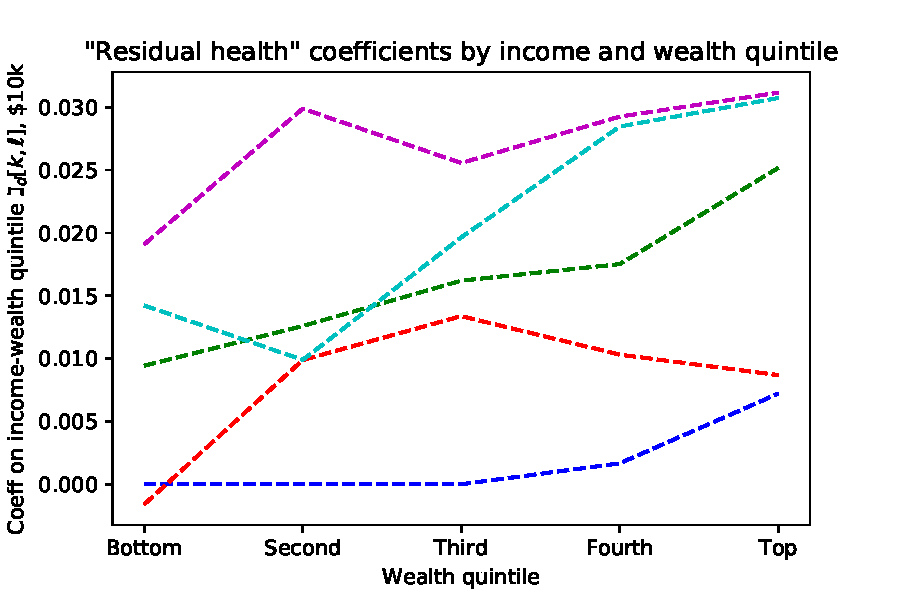
\includegraphics[width=\textwidth]{../Figures/HealthCoeffByIncWealthDataOnly.pdf}
        \caption{HRS data moments, category 7(a)}
    \end{subfigure}
    \begin{subfigure}[b]{0.49\textwidth}
        \centering
        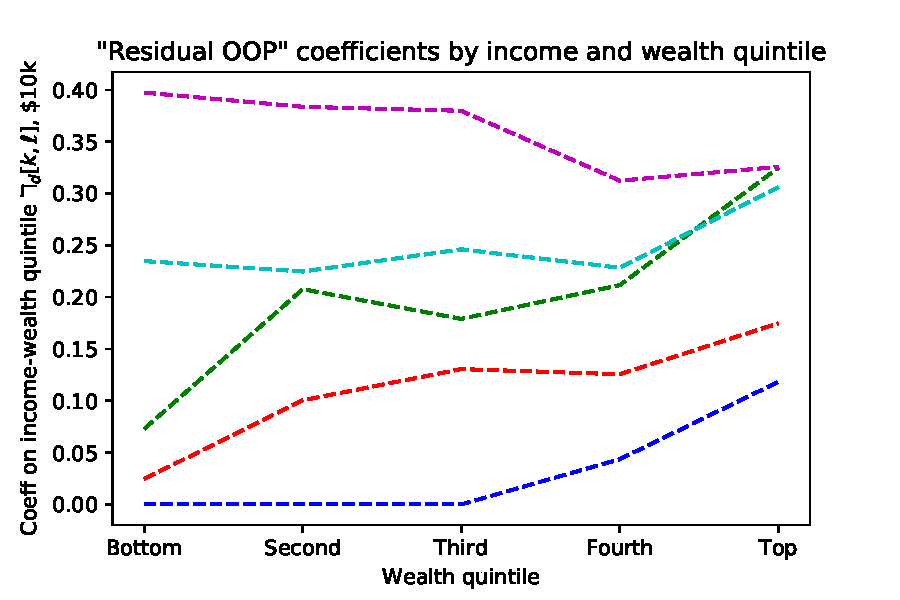
\includegraphics[width=\textwidth]{../Figures/OOPcoeffByIncWealthDataOnly.pdf}
        \caption{HRS data moments, category 7(b)}
    \end{subfigure}
    \caption{HRS data for category 7 moments; see equations \eqref{HealthOLS} and \eqref{OOPOLS}.}
    \label{fig:MomentCat7DataOnly}
\end{figure}


\newpage


\begin{figure}[h!]
    \centering
    \begin{subfigure}[b]{0.49\textwidth}
        \centering
        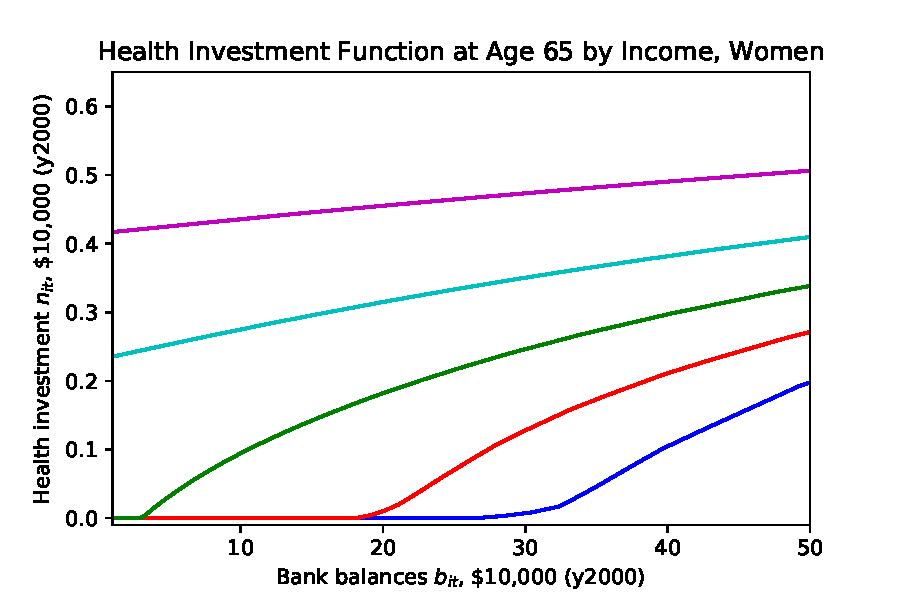
\includegraphics[width=\textwidth]{../Figures/iFuncWomen.pdf}
        \caption{Health investment functions for women}
    \end{subfigure}
    \begin{subfigure}[b]{0.49\textwidth}
        \centering
        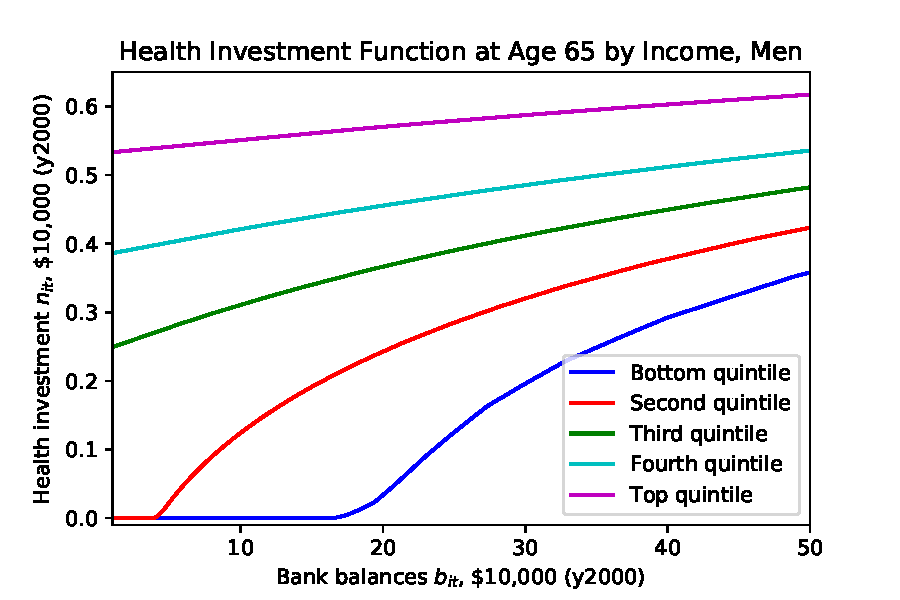
\includegraphics[width=\textwidth]{../Figures/iFuncMen.pdf}
        \caption{Health investment functions for men}
    \end{subfigure}
    \caption{Health investment policy functions by income-sex type at age 65 in estimated model, with health capital at $\Health_{it}=0.6$ and medical need shock $\MedShk_{it}$ at its mean value.}
    \label{fig:iFunc}
\end{figure}


\begin{figure}[h!]
    \centering
    \begin{subfigure}[b]{0.49\textwidth}
        \centering
        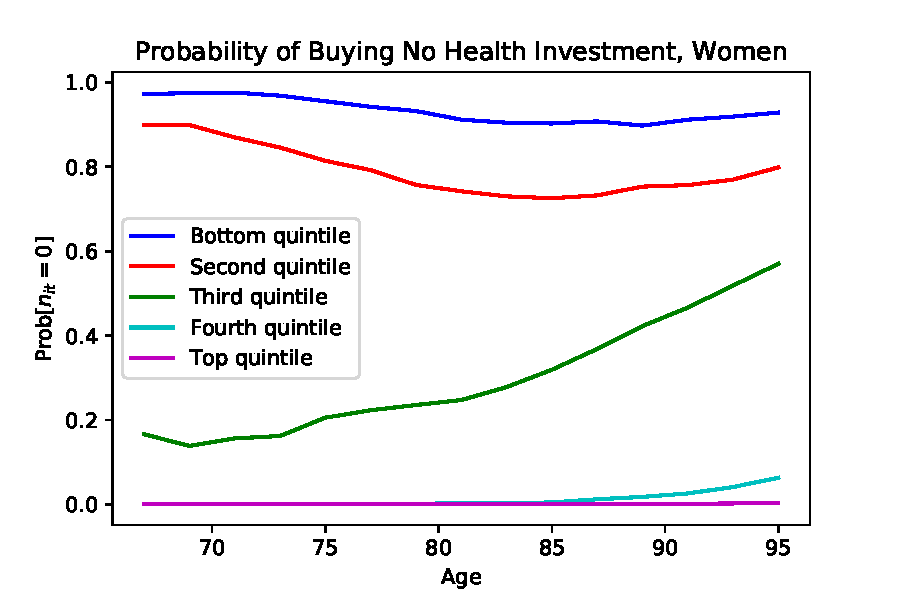
\includegraphics[width=\textwidth]{../Figures/ZeroInvstWomen.pdf}
        \caption{Probability of $\Invst_{it}=0$, women}
    \end{subfigure}
    \begin{subfigure}[b]{0.49\textwidth}
        \centering
        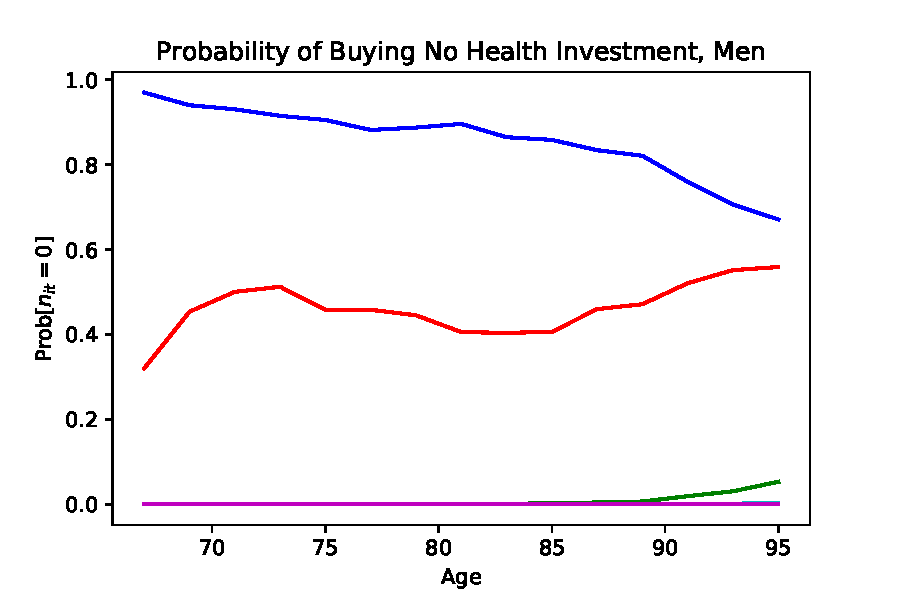
\includegraphics[width=\textwidth]{../Figures/ZeroInvstMen.pdf}
        \caption{Probability of $\Invst_{it}=0$, men}
    \end{subfigure}
    \begin{subfigure}[b]{0.49\textwidth}
        \centering
        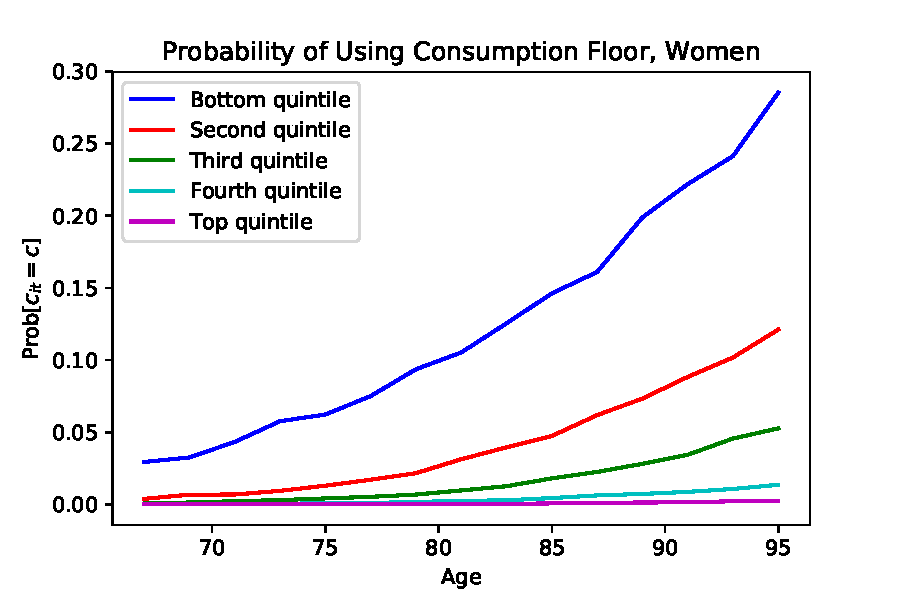
\includegraphics[width=\textwidth]{../Figures/cFloorWomen.pdf}
        \caption{Probability of $\Con_{it}=\ConFloor$, women}
    \end{subfigure}
    \begin{subfigure}[b]{0.49\textwidth}
        \centering
        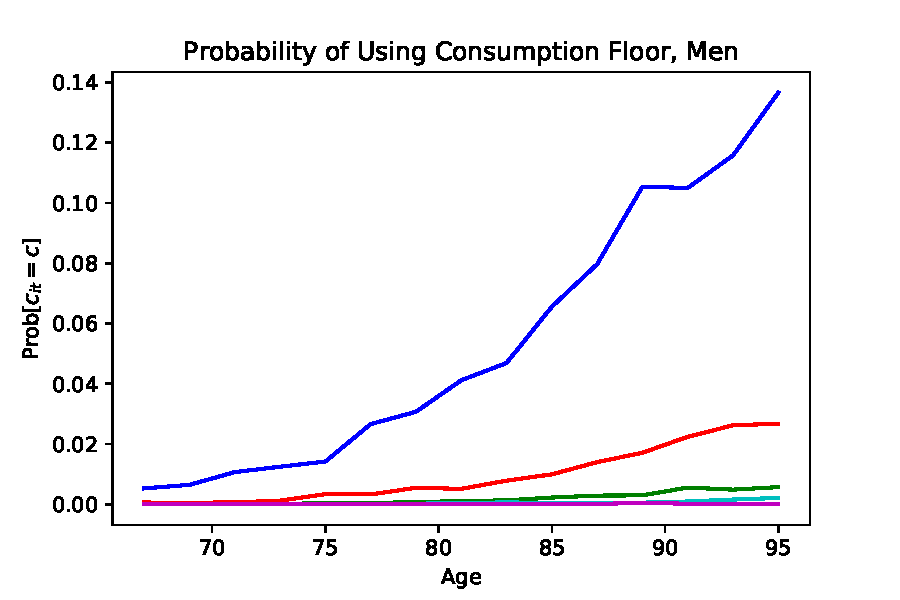
\includegraphics[width=\textwidth]{../Figures/cFloorMen.pdf}
        \caption{Probability of $\Con_{it}=\ConFloor$, men}
    \end{subfigure}
    \caption{Fraction of model retirees who purchase no health investment or use the consumption floor by age, sex, and income.}
    \label{fig:ZeroInvstAndConFloor}
\end{figure}


\newpage


\begin{figure}[h!]
\begin{center}
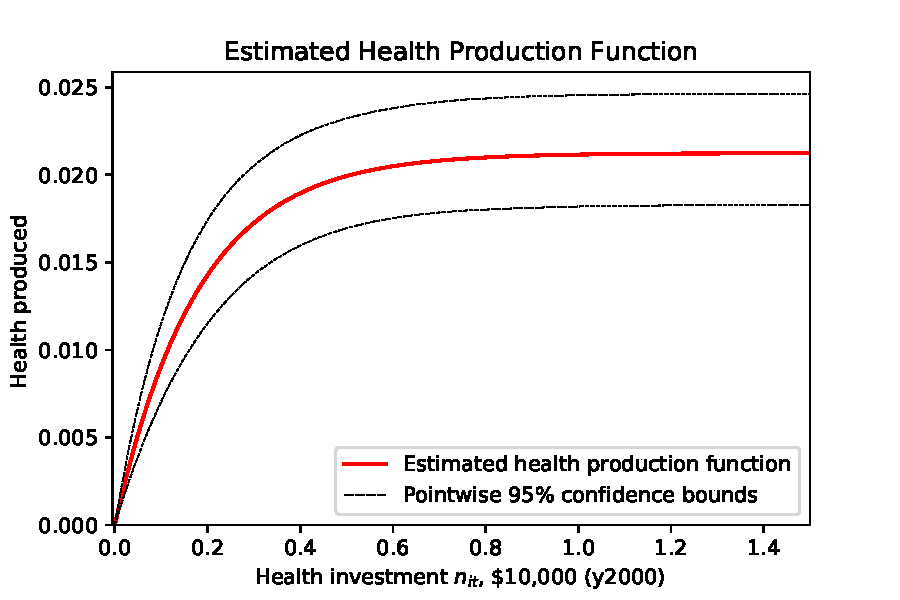
\includegraphics[scale=0.9]{../Figures/HealthProdFunc.pdf}
\end{center}
\vspace{-0.5cm}
\caption{Estimated health production function with 95\% confidence bands}
\label{fig:HealthProdFunc}
\end{figure}

\begin{figure}[h!]
\begin{center}
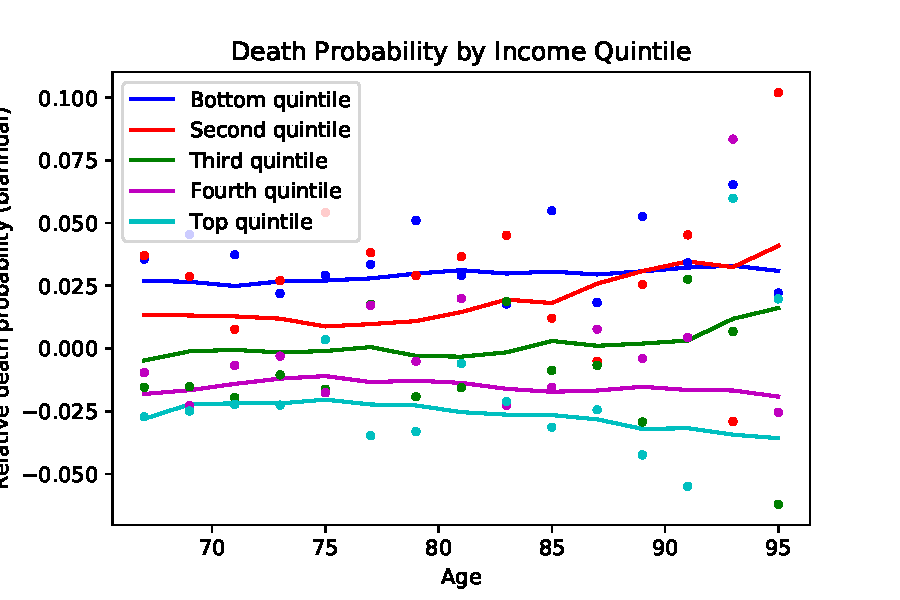
\includegraphics[scale=0.9]{../Figures/MortByIncAge.pdf}
\end{center}
\vspace{-0.5cm}
\caption{Two-year (relative) mortality probability by income quintile age, removing age trend, in HRS data (dots) and estimated model (solid lines)}
\label{fig:MortByIncAge}
\end{figure}


\newpage

\begin{figure}[h!]
\begin{center}
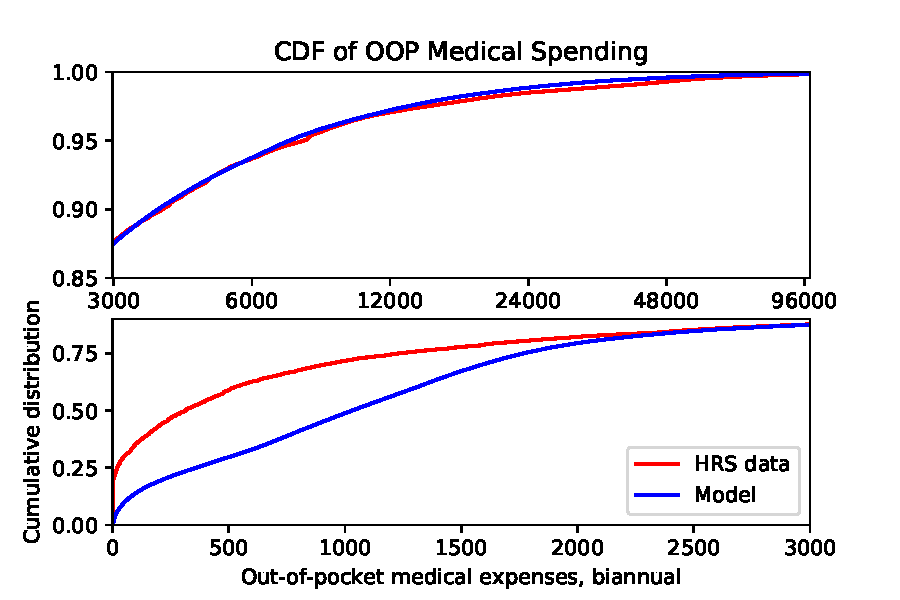
\includegraphics[scale=0.9]{../Figures/OOPdistribution.pdf}
\end{center}
\vspace{-0.5cm}
\caption{Overall distribution of OOP medical expenses in HRS data vs estimated model}
\label{fig:OOPdistribution}
\end{figure}

\begin{figure}[h!]
\begin{center}
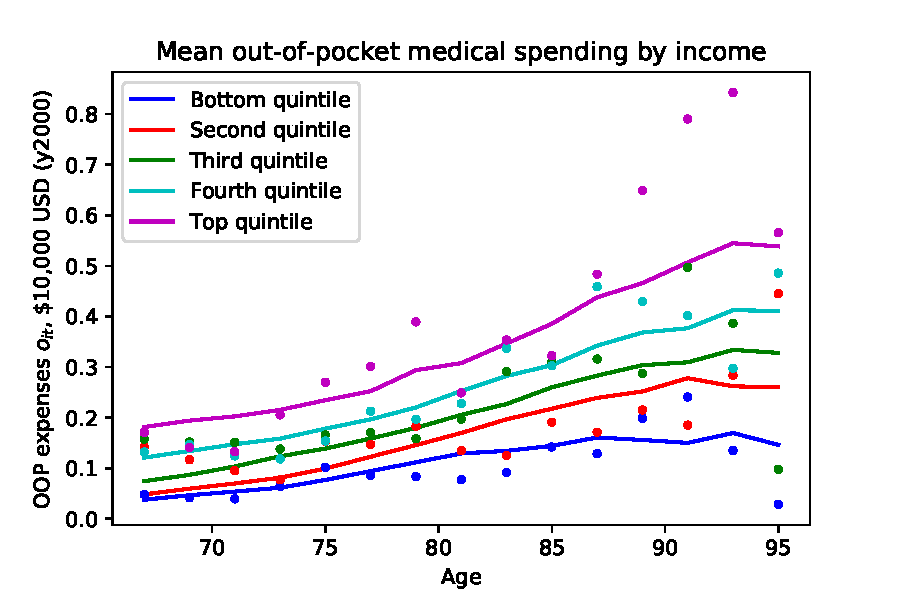
\includegraphics[scale=0.9]{../Figures/OOPbyIncAge.pdf}
\end{center}
\vspace{-0.5cm}
\caption{Mean OOP medical expenses by age and income quintile in HRS data (dashed) vs estimated model (solid)}
\label{fig:OOPbyIncAge}
\end{figure}

\begin{figure}[h!]
\begin{center}
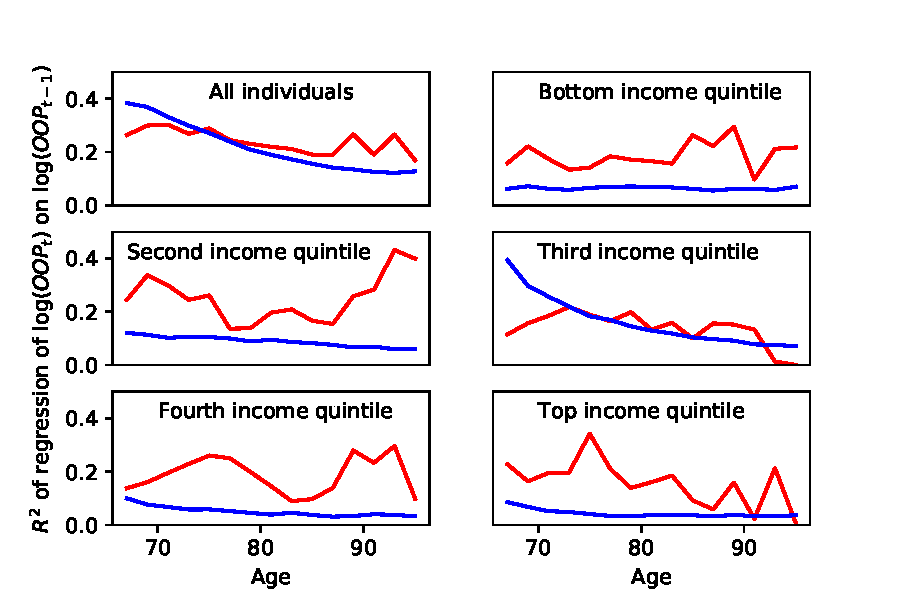
\includegraphics[scale=0.9]{../Figures/SerialCorrOOP.pdf}
\end{center}
\vspace{-0.5cm}
\caption{Serial correlation of OOP medical expenses by age and income quintile}
\label{fig:SerialCorrOOP}
\end{figure}

\begin{figure}[ht!]
    \centering
    \begin{subfigure}[b]{0.49\textwidth}
        \centering
        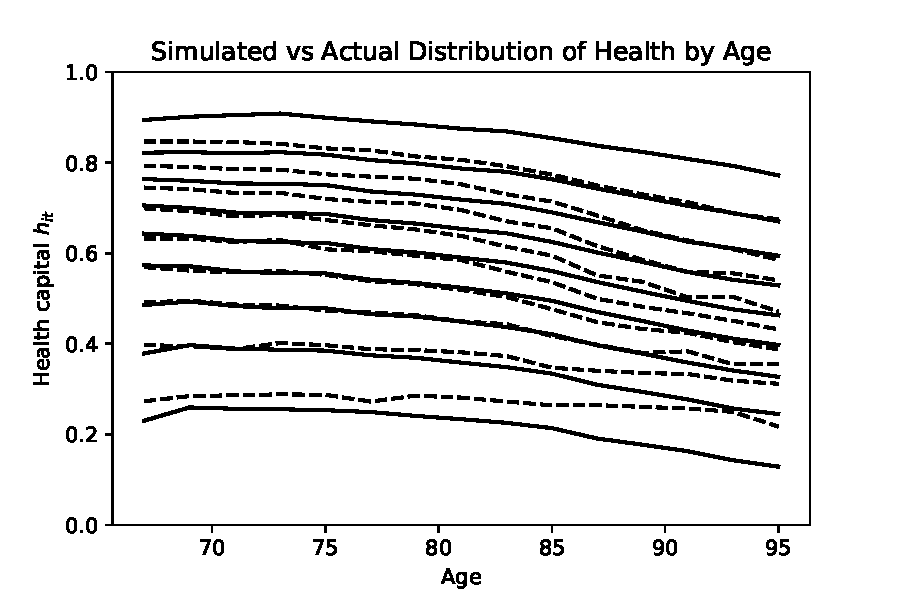
\includegraphics[width=\textwidth]{../Figures/HealthDistribution.pdf}
        \caption{Estimated parameters}
    \end{subfigure}
    \begin{subfigure}[b]{0.49\textwidth}
        \centering
        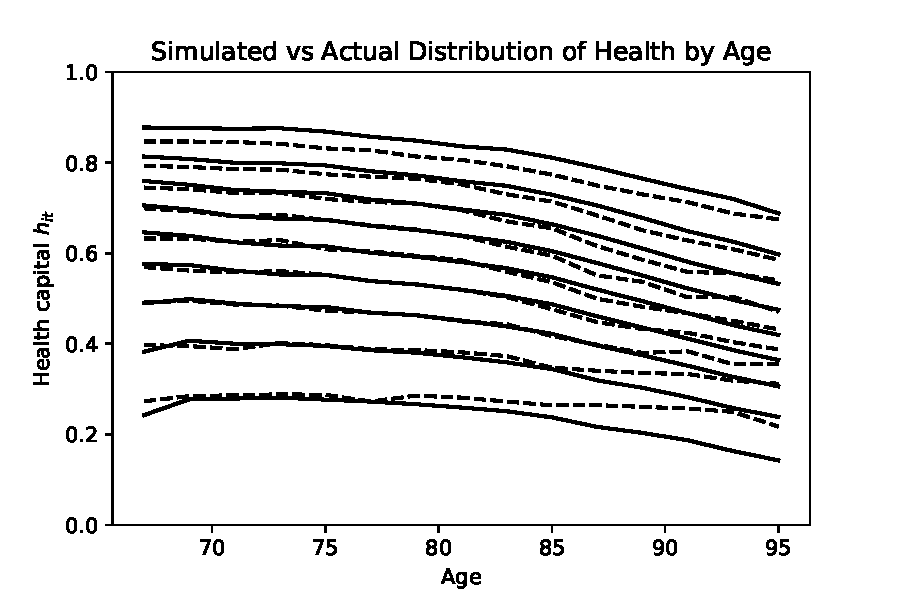
\includegraphics[width=\textwidth]{../Figures/HealthDistributionAlt.pdf}
        \caption{$\HealthParam_{\sigma 0}$ and $\HealthParam_{\sigma 1}$ reduced by 25\%}
    \end{subfigure}
    \caption{Overall health distribution by age in the HRS data (dots) vs simulated model (solid), at the 10th-90th percentiles}
    \label{fig:HealthDistribution}
\end{figure}

\begin{figure}[h!]
   \centering
   \begin{subfigure}[b]{0.49\textwidth}
      \centering
      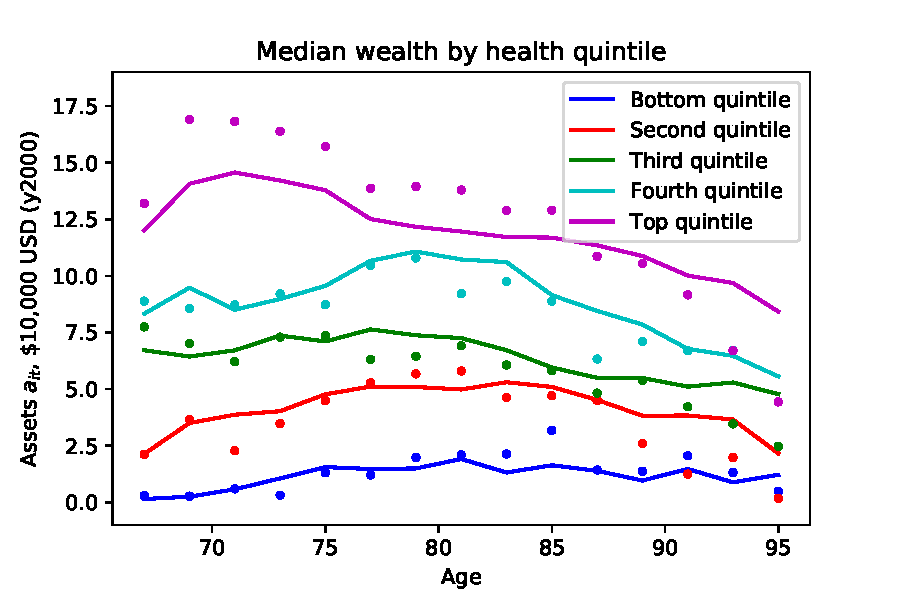
\includegraphics[width=\textwidth]{../Figures/WealthByHealthAge.pdf}
   \end{subfigure}
   \begin{subfigure}[b]{0.49\textwidth}
      \centering
      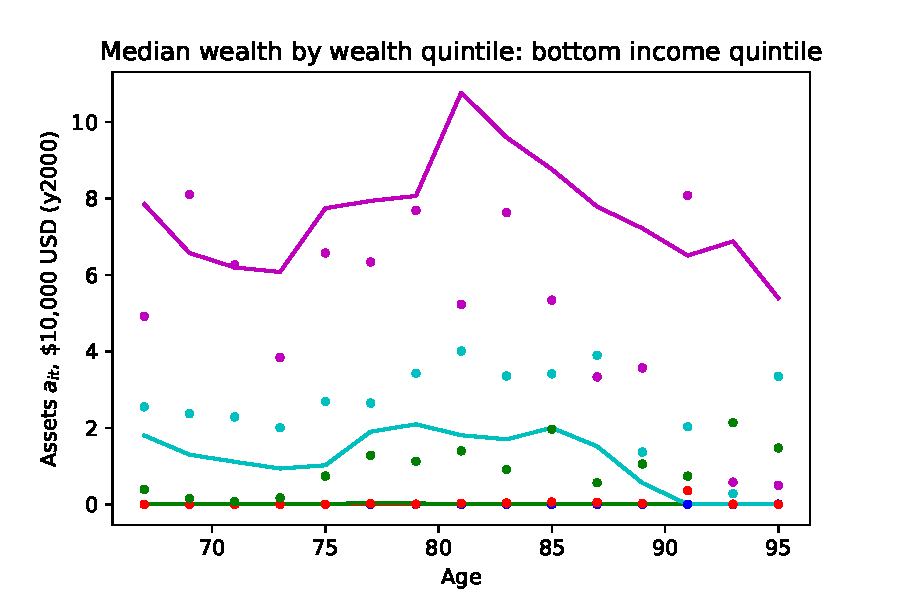
\includegraphics[width=\textwidth]{../Figures/WealthByIncWealthAge1.pdf}
   \end{subfigure}
   \begin{subfigure}[b]{0.49\textwidth}
      \centering
      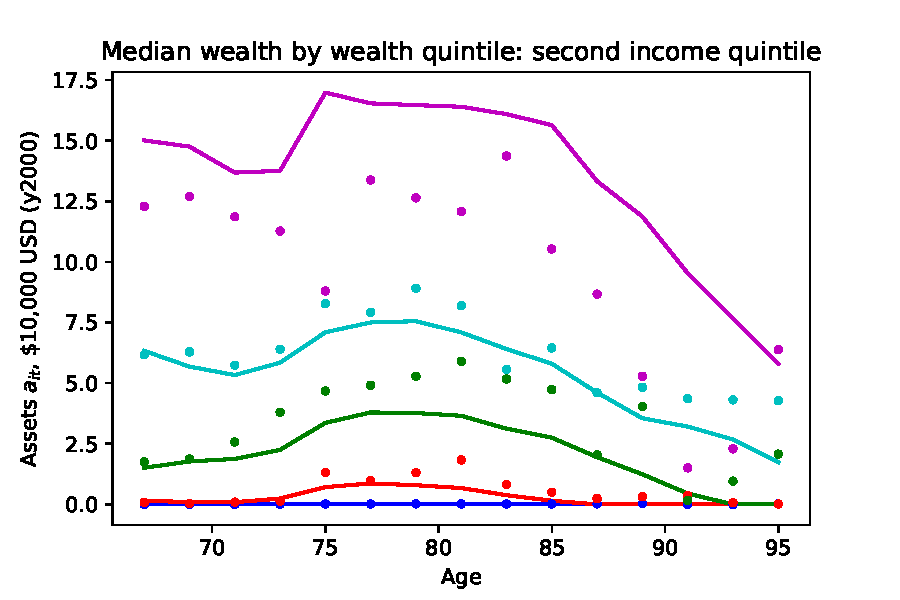
\includegraphics[width=\textwidth]{../Figures/WealthByIncWealthAge2.pdf}
   \end{subfigure}
   \begin{subfigure}[b]{0.49\textwidth}
      \centering
      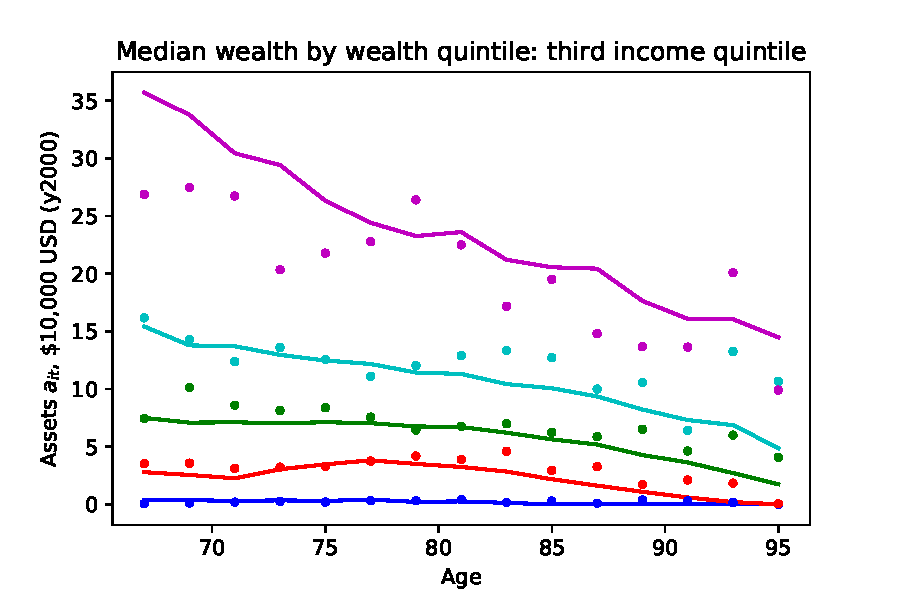
\includegraphics[width=\textwidth]{../Figures/WealthByIncWealthAge3.pdf}
   \end{subfigure}
   \begin{subfigure}[b]{0.49\textwidth}
      \centering
      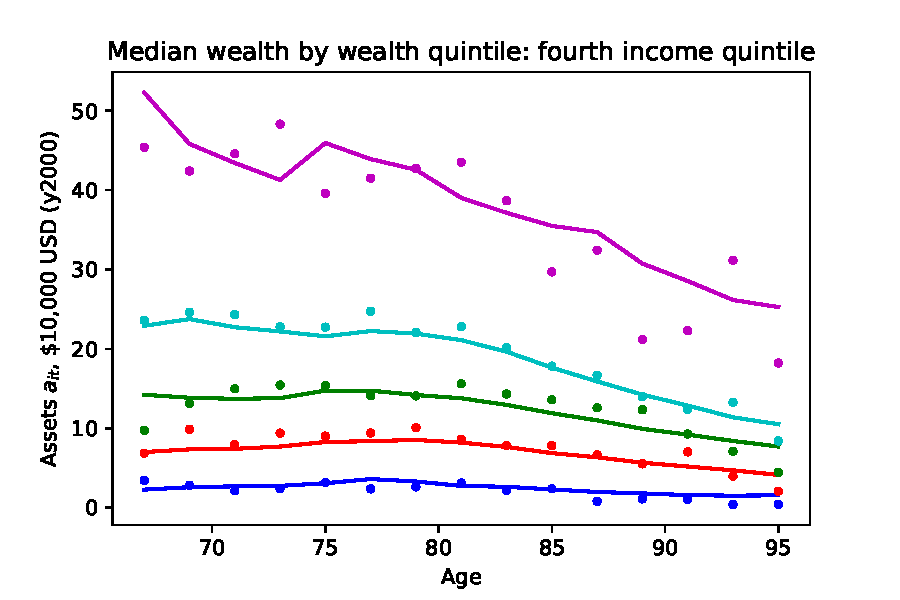
\includegraphics[width=\textwidth]{../Figures/WealthByIncWealthAge4.pdf}
   \end{subfigure}
   \begin{subfigure}[b]{0.49\textwidth}
      \centering
      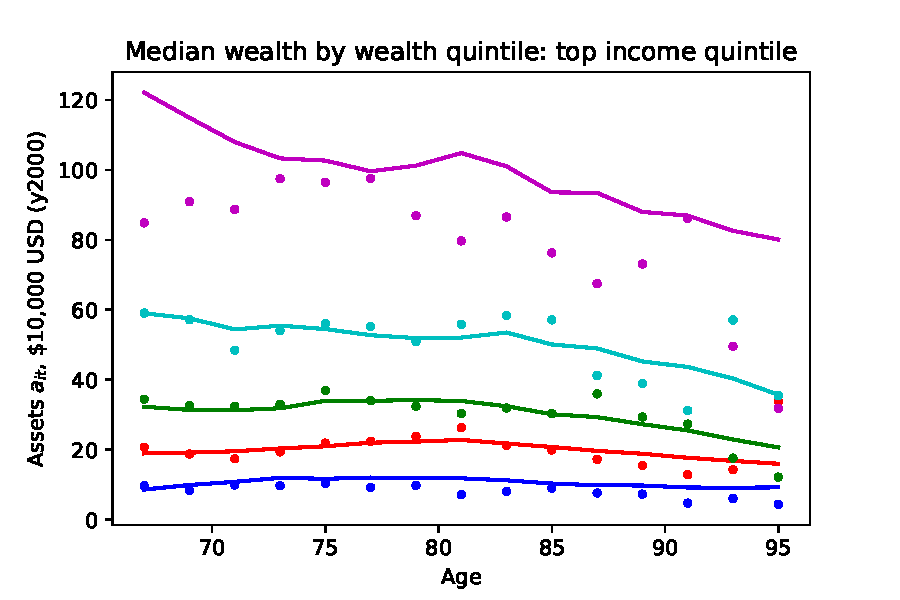
\includegraphics[width=\textwidth]{../Figures/WealthByIncWealthAge5.pdf}
   \end{subfigure}
   \caption{Wealth profiles by subpopulation in HRS data (dots) vs estimated model (lines)}
   \label{fig:WealthBySubpop}
\end{figure}


\newpage

\begin{figure}[h!]
    \centering
    \begin{subfigure}[b]{0.49\textwidth}
        \centering
        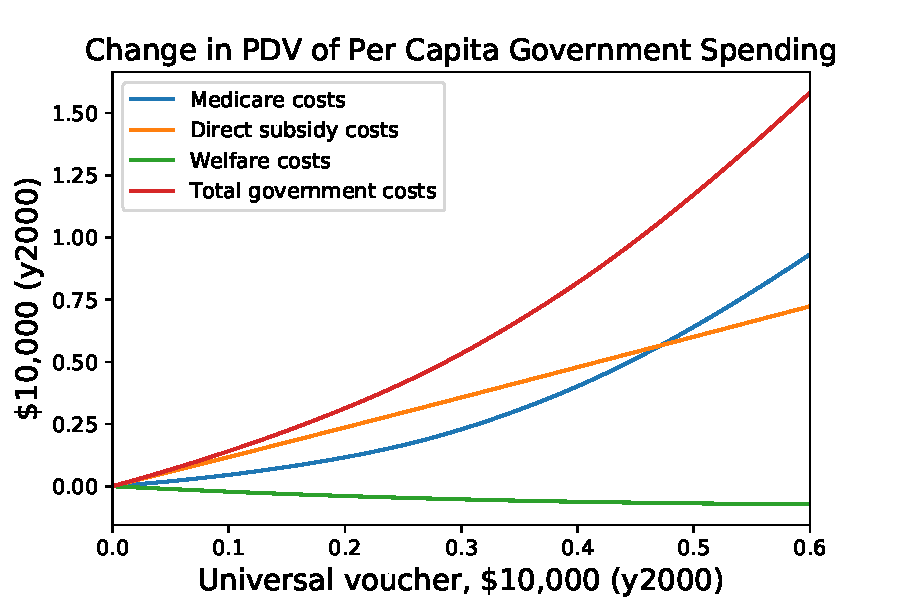
\includegraphics[width=\textwidth]{../Figures/UniversalSubGovtChange.pdf}
        \caption{Change in government expenditures}
    \end{subfigure}
    \begin{subfigure}[b]{0.49\textwidth}
        \centering
        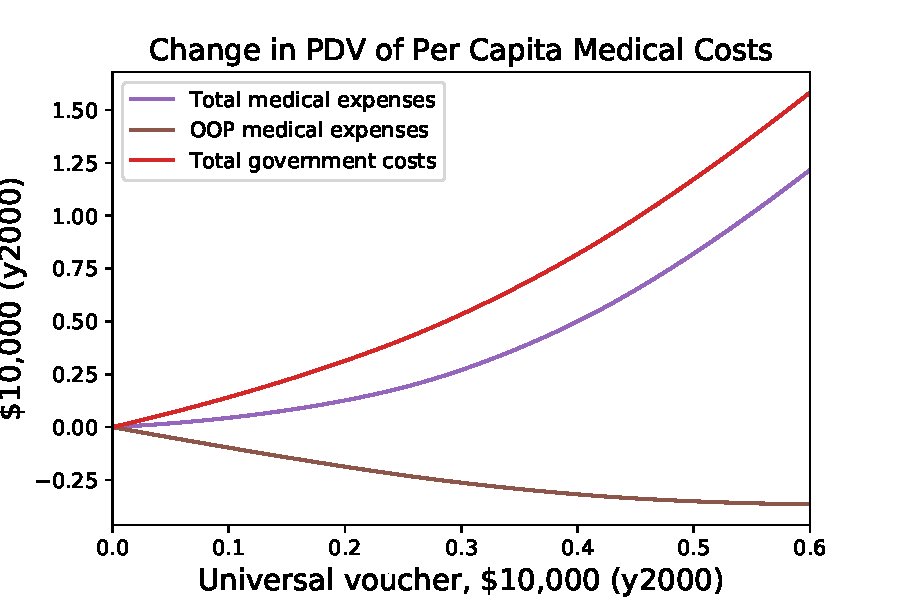
\includegraphics[width=\textwidth]{../Figures/UniversalSubMedChange.pdf}
        \caption{Change in composition of medical spending}
    \end{subfigure}
    \begin{subfigure}[b]{0.49\textwidth}
        \centering
        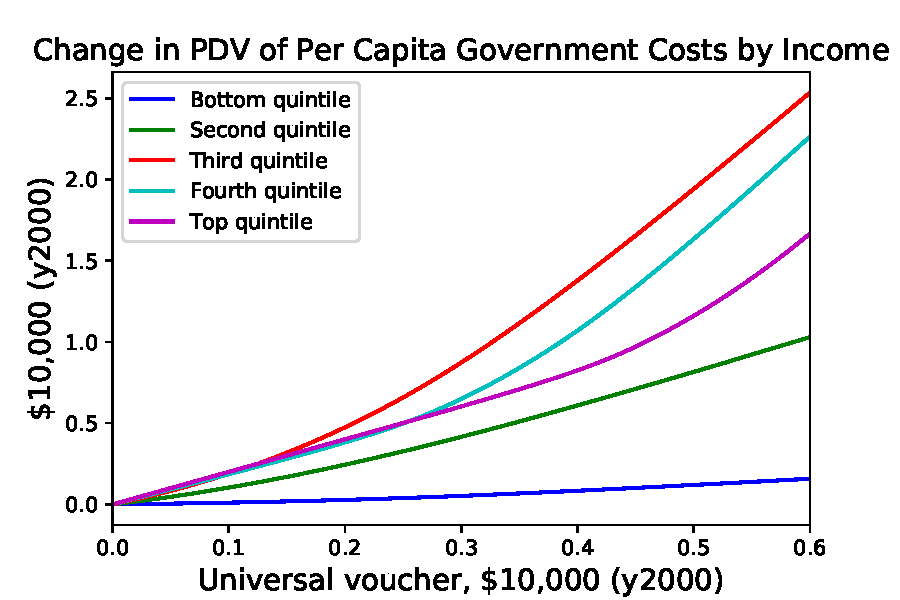
\includegraphics[width=\textwidth]{../Figures/UniversalSubGovtChangeByInc.pdf}
        \caption{Change in government spending by income}
    \end{subfigure}
    \begin{subfigure}[b]{0.49\textwidth}
        \centering
        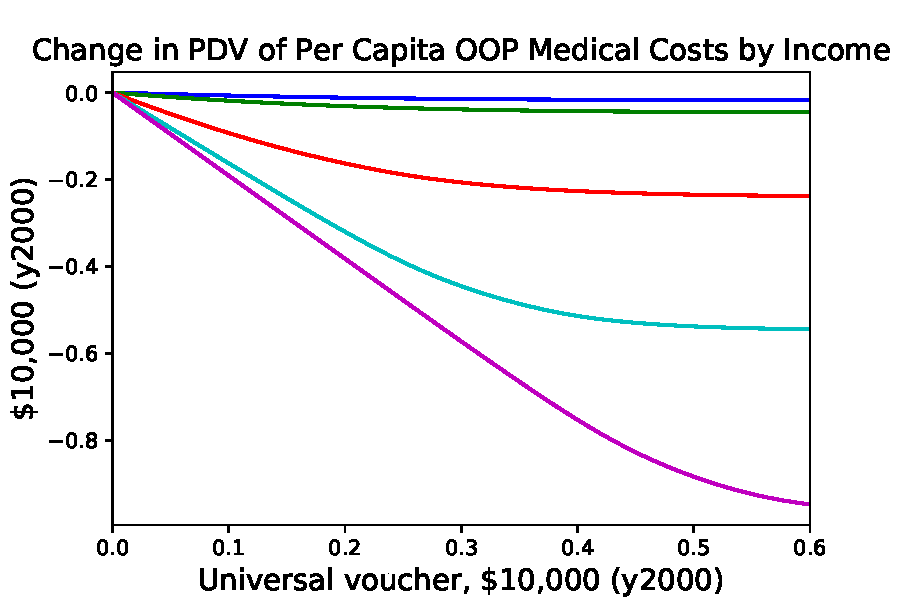
\includegraphics[width=\textwidth]{../Figures/UniversalSubOOPchangeByInc.pdf}
        \caption{Change in out-of-pocket expenses by income}
    \end{subfigure}
    \begin{subfigure}[b]{0.49\textwidth}
        \centering
        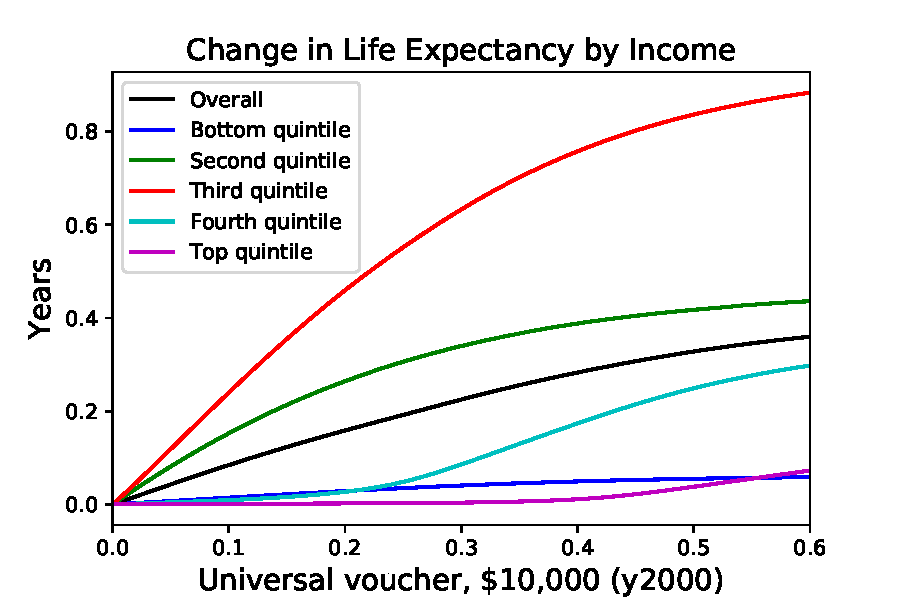
\includegraphics[width=\textwidth]{../Figures/UniversalSubLifeExp.pdf}
        \caption{Change in life expectancy}
    \end{subfigure}
    \begin{subfigure}[b]{0.49\textwidth}
        \centering
        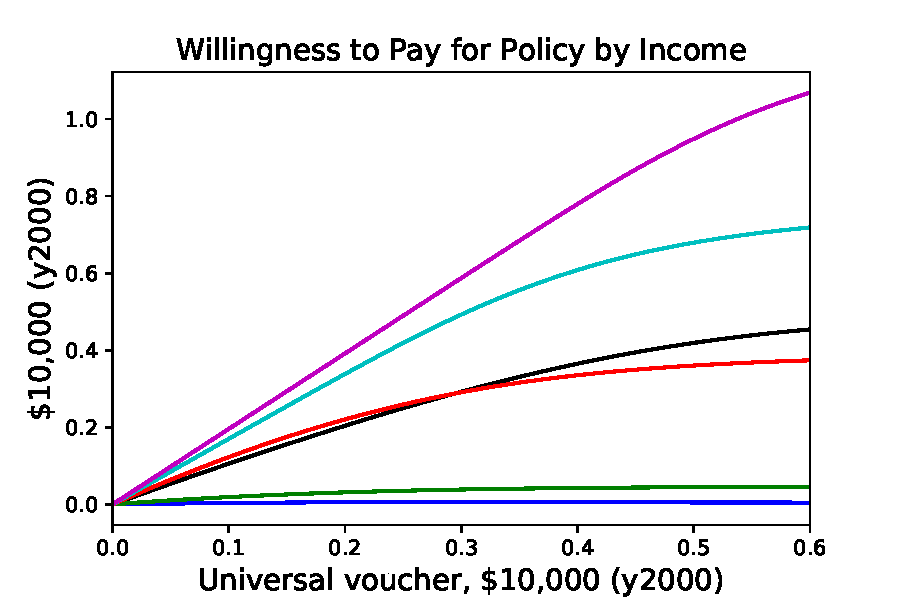
\includegraphics[width=\textwidth]{../Figures/UniversalSubWTP.pdf}
        \caption{Willingness to pay for policy}
    \end{subfigure}
    \caption{Counterfactual experiment: Direct, universal subsidy covering fixed quantity of health investment per period}
    \label{fig:UniversalSub}
\end{figure}


\newpage


\begin{figure}[h!]
    \centering
    \begin{subfigure}[b]{0.49\textwidth}
        \centering
        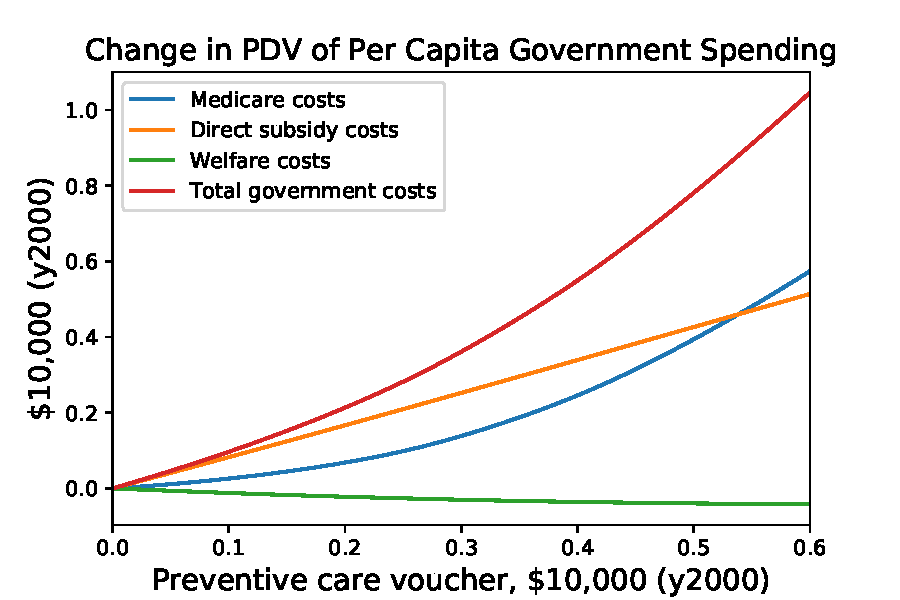
\includegraphics[width=\textwidth]{../Figures/PreventiveSubGovtChange.pdf}
        \caption{Change in government expenditures}
    \end{subfigure}
    \begin{subfigure}[b]{0.49\textwidth}
        \centering
        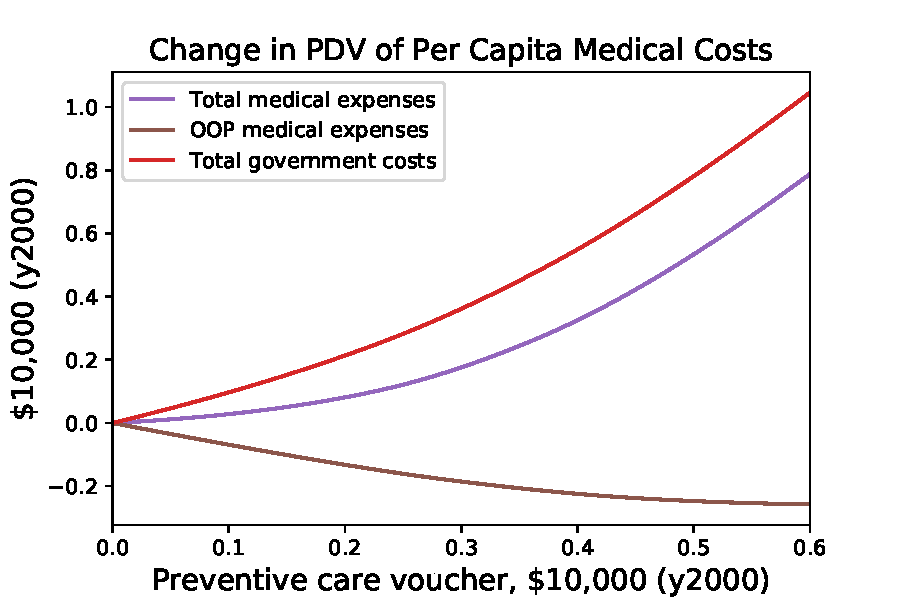
\includegraphics[width=\textwidth]{../Figures/PreventiveSubMedChange.pdf}
        \caption{Change in composition of medical spending}
    \end{subfigure}
    \begin{subfigure}[b]{0.49\textwidth}
        \centering
        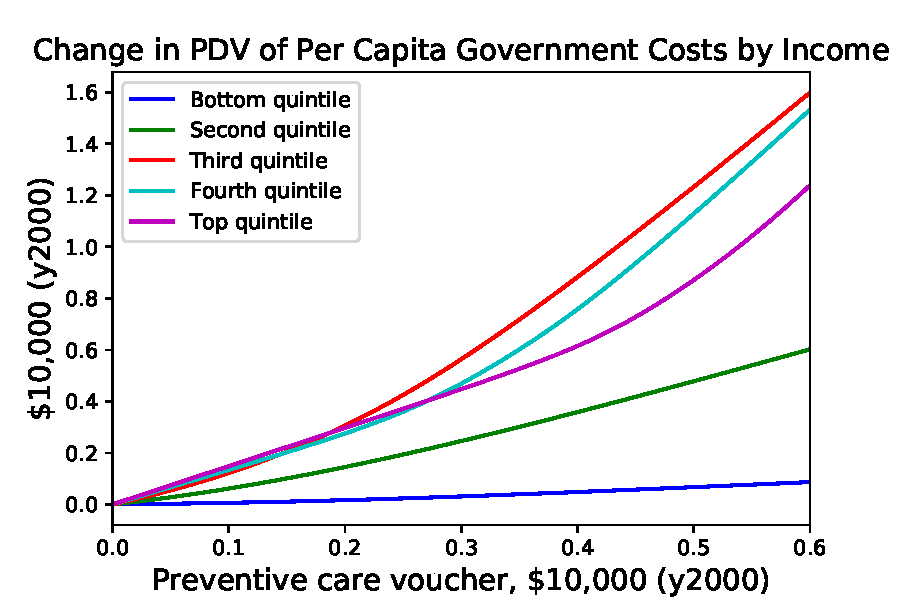
\includegraphics[width=\textwidth]{../Figures/PreventiveSubGovtChangeByInc.pdf}
        \caption{Change in government spending by income}
    \end{subfigure}
    \begin{subfigure}[b]{0.49\textwidth}
        \centering
        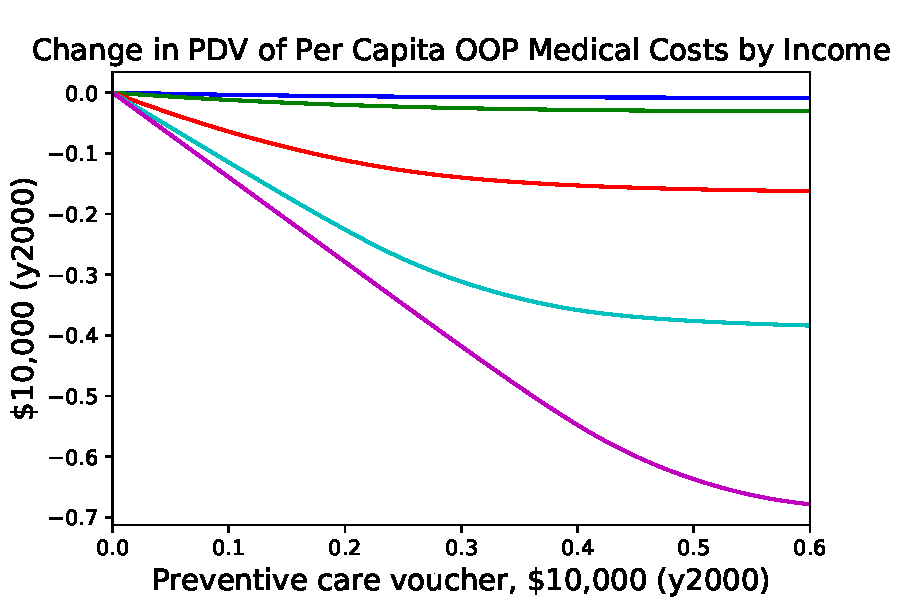
\includegraphics[width=\textwidth]{../Figures/PreventiveSubOOPchangeByInc.pdf}
        \caption{Change in out-of-pocket expenses by income}
    \end{subfigure}
    \begin{subfigure}[b]{0.49\textwidth}
        \centering
        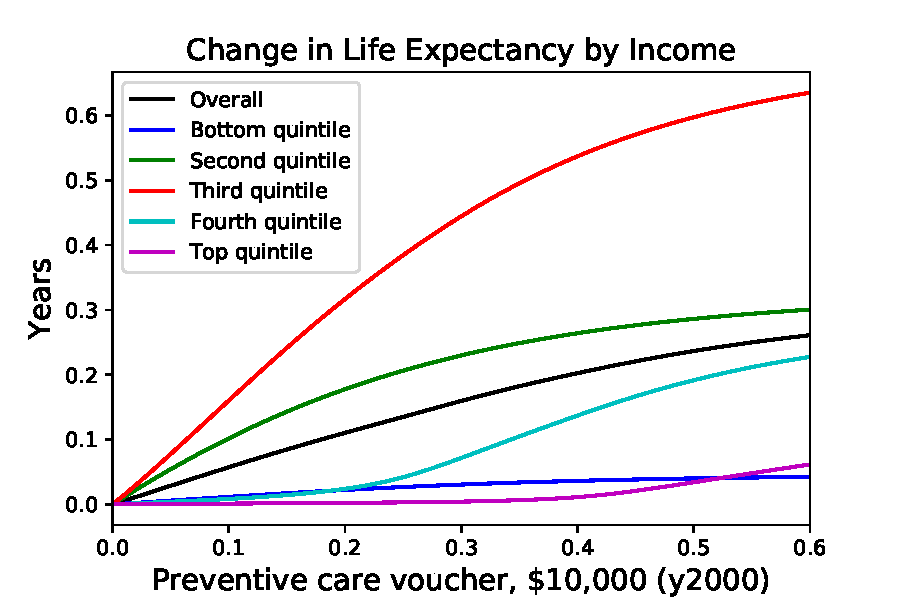
\includegraphics[width=\textwidth]{../Figures/PreventiveSubLifeExp.pdf}
        \caption{Change in life expectancy}
    \end{subfigure}
    \begin{subfigure}[b]{0.49\textwidth}
        \centering
        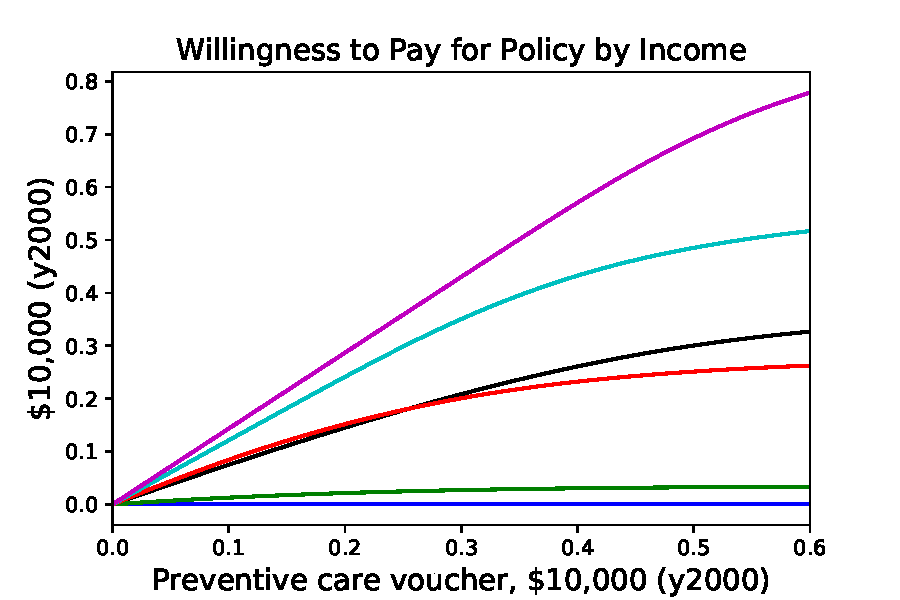
\includegraphics[width=\textwidth]{../Figures/PreventiveSubWTP.pdf}
        \caption{Willingness to pay for policy}
    \end{subfigure}
    \caption{Counterfactual experiment: Direct subsidy covering fixed quantity of health investment per period, conditional on $\Health_{it} \geq 0$.}
    \label{fig:PreventiveSub}
\end{figure}


\begin{figure}[h!]
    \centering
    \begin{subfigure}[b]{0.49\textwidth}
        \centering
        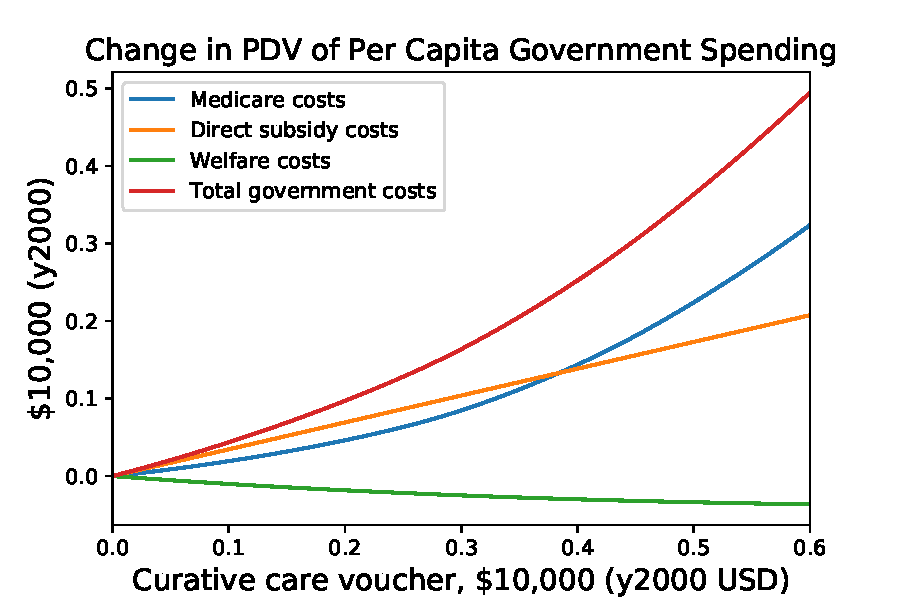
\includegraphics[width=\textwidth]{../Figures/CurativeSubGovtChange.pdf}
        \caption{Change in government expenditures}
    \end{subfigure}
    \begin{subfigure}[b]{0.49\textwidth}
        \centering
        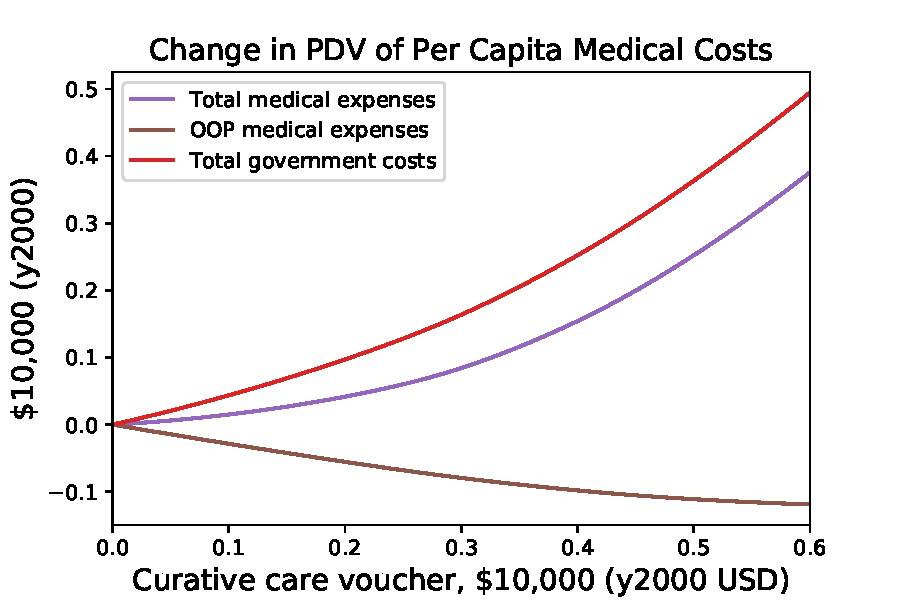
\includegraphics[width=\textwidth]{../Figures/CurativeSubMedChange.pdf}
        \caption{Change in composition of medical spending}
    \end{subfigure}
    \begin{subfigure}[b]{0.49\textwidth}
        \centering
        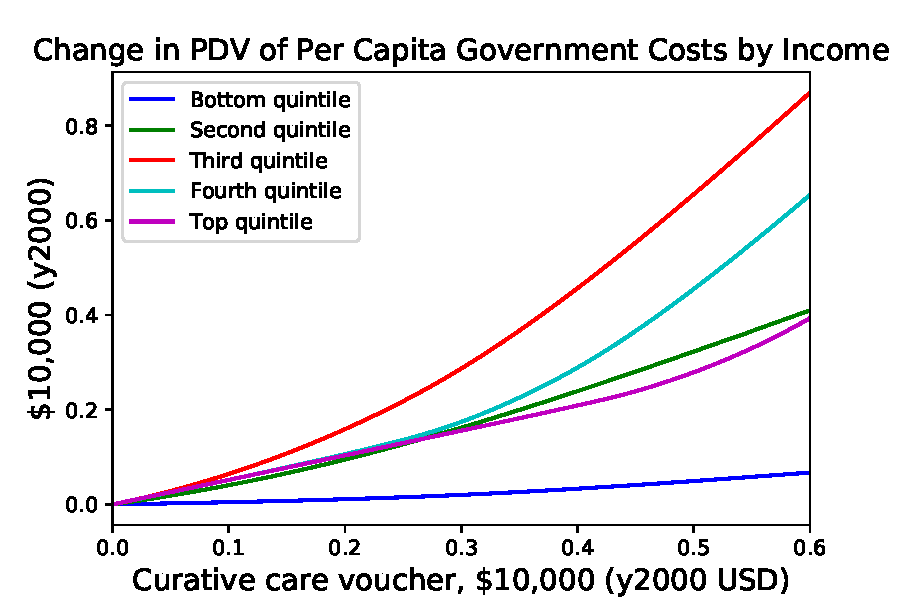
\includegraphics[width=\textwidth]{../Figures/CurativeSubGovtChangeByInc.pdf}
        \caption{Change in government spending by income}
    \end{subfigure}
    \begin{subfigure}[b]{0.49\textwidth}
        \centering
        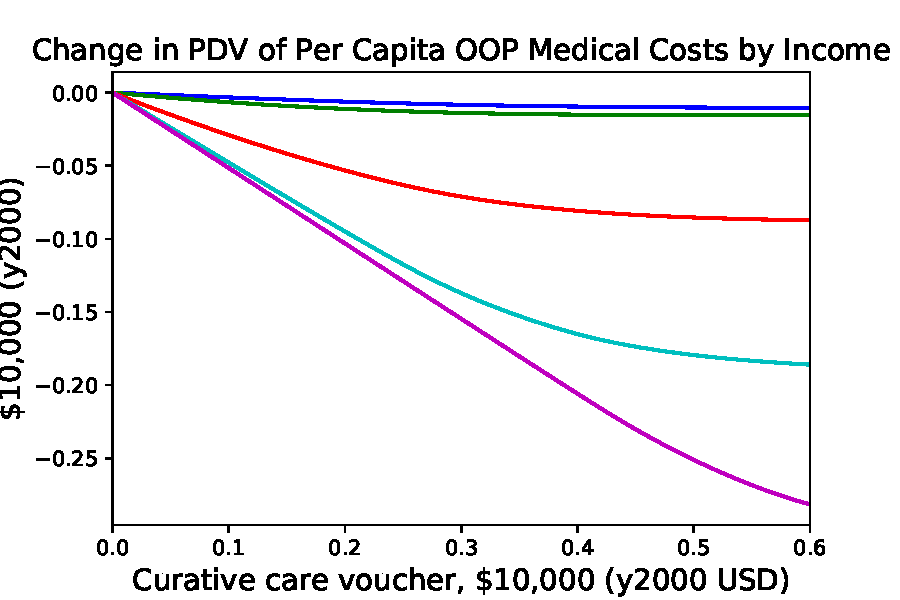
\includegraphics[width=\textwidth]{../Figures/CurativeSubOOPchangeByInc.pdf}
        \caption{Change in out-of-pocket expenses by income}
    \end{subfigure}
    \begin{subfigure}[b]{0.49\textwidth}
        \centering
        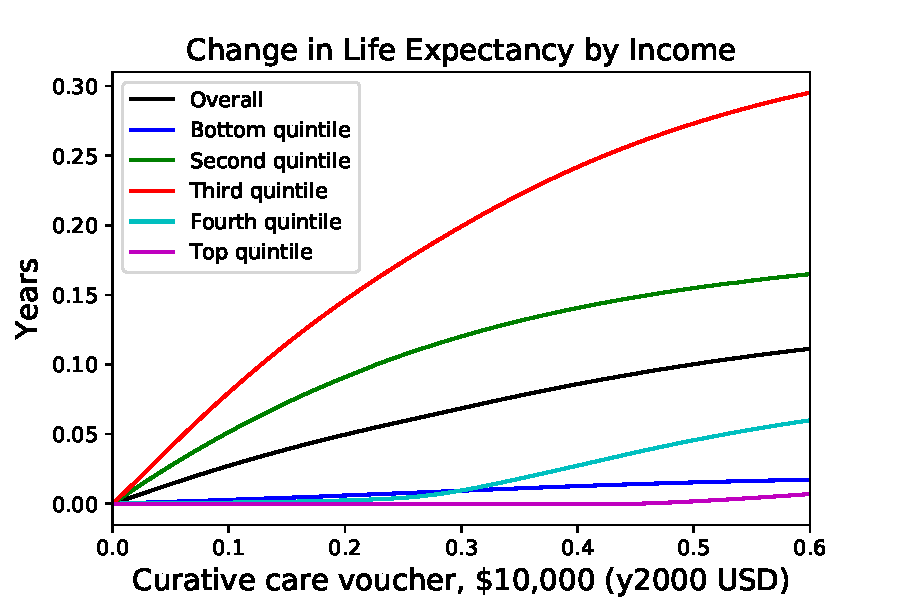
\includegraphics[width=\textwidth]{../Figures/CurativeSubLifeExp.pdf}
        \caption{Change in life expectancy}
    \end{subfigure}
    \begin{subfigure}[b]{0.49\textwidth}
        \centering
        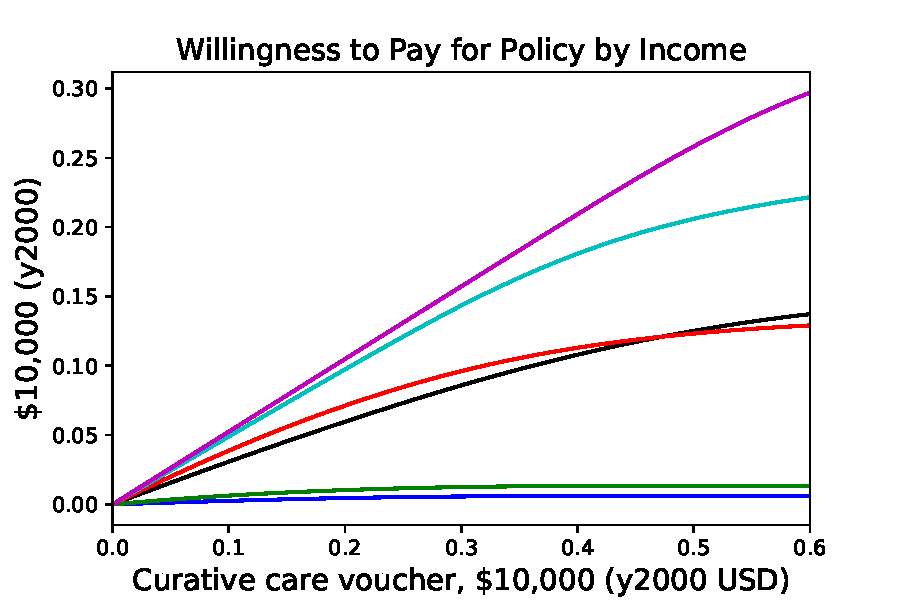
\includegraphics[width=\textwidth]{../Figures/CurativeSubWTP.pdf}
        \caption{Willingness to pay for policy}
    \end{subfigure}
    \caption{Counterfactual experiment: Direct subsidy covering fixed quantity of health investment per period, conditional on $\Health_{it} \leq 0$.}
    \label{fig:CurativeSub}
\end{figure}


\newpage


\begin{figure}[h!]
    \centering
    \begin{subfigure}[b]{0.49\textwidth}
        \centering
        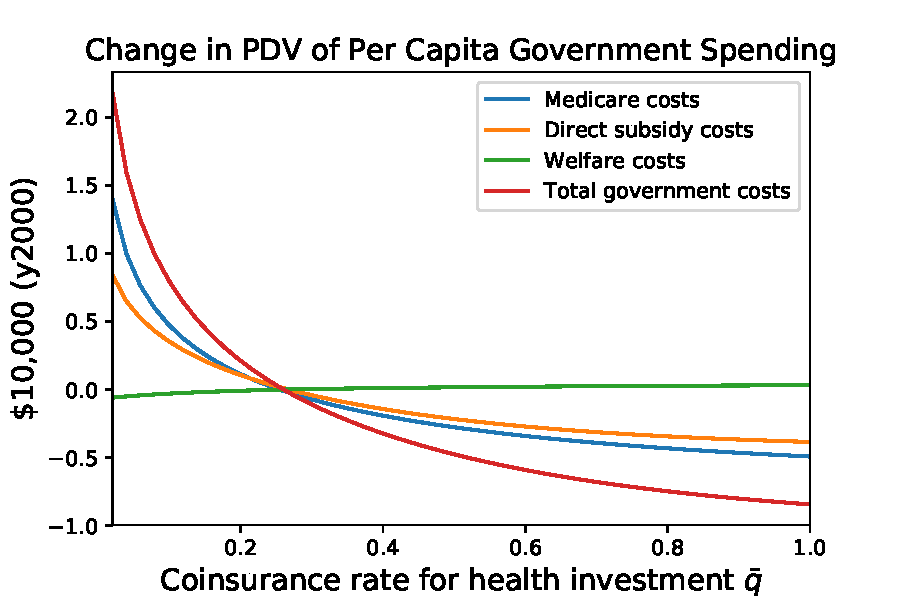
\includegraphics[width=\textwidth]{../Figures/FlatCopayInvstGovtChange.pdf}
        \caption{Change in government expenditures}
    \end{subfigure}
    \begin{subfigure}[b]{0.49\textwidth}
        \centering
        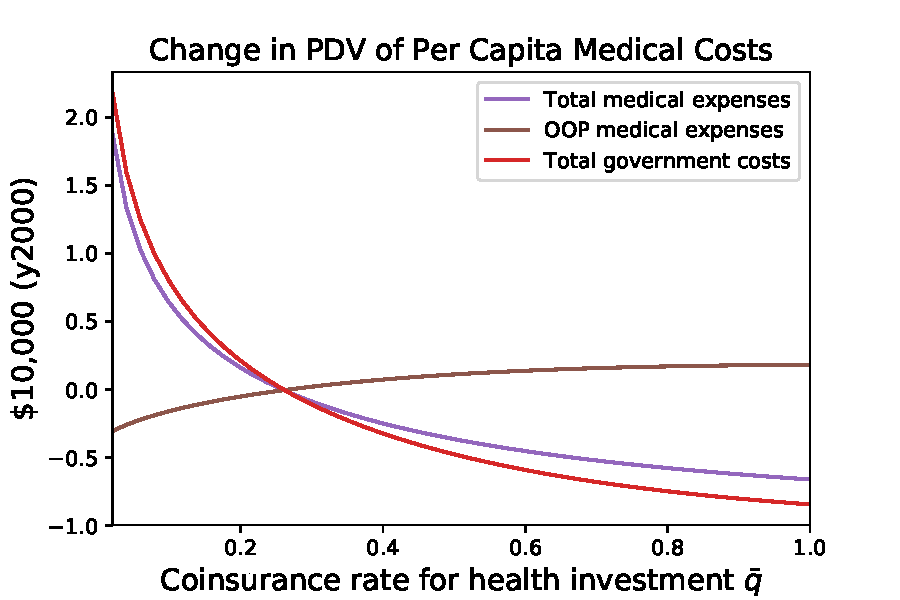
\includegraphics[width=\textwidth]{../Figures/FlatCopayInvstMedChange.pdf}
        \caption{Change in composition of medical spending}
    \end{subfigure}
    \begin{subfigure}[b]{0.49\textwidth}
        \centering
        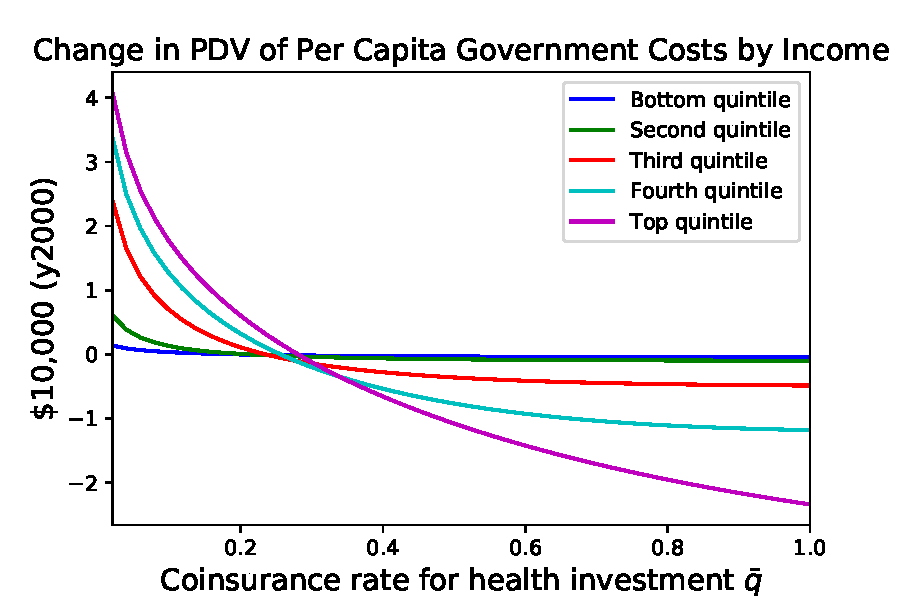
\includegraphics[width=\textwidth]{../Figures/FlatCopayInvstGovtChangeByInc.pdf}
        \caption{Change in government spending by income}
    \end{subfigure}
    \begin{subfigure}[b]{0.49\textwidth}
        \centering
        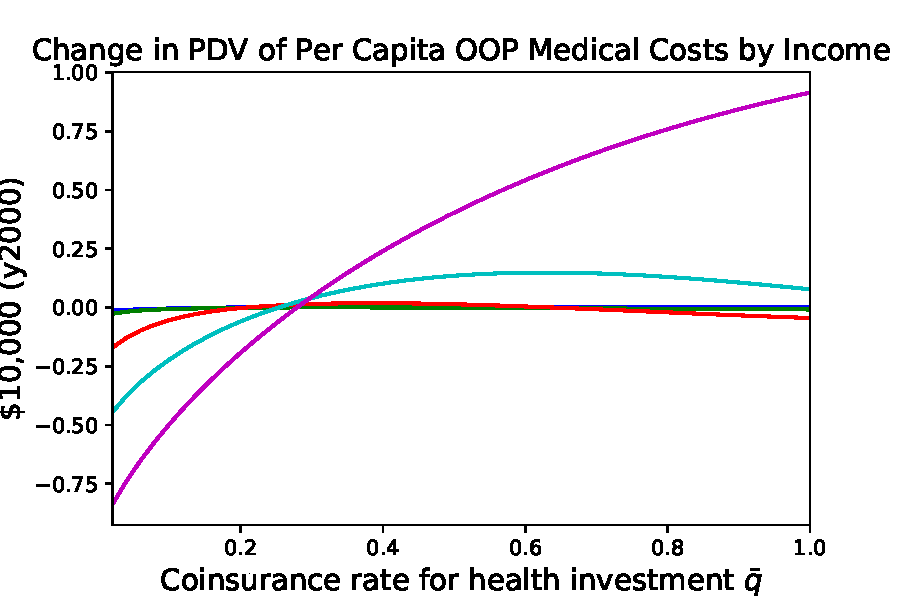
\includegraphics[width=\textwidth]{../Figures/FlatCopayInvstOOPchangeByInc.pdf}
        \caption{Change in out-of-pocket expenses by income}
    \end{subfigure}
    \begin{subfigure}[b]{0.49\textwidth}
        \centering
        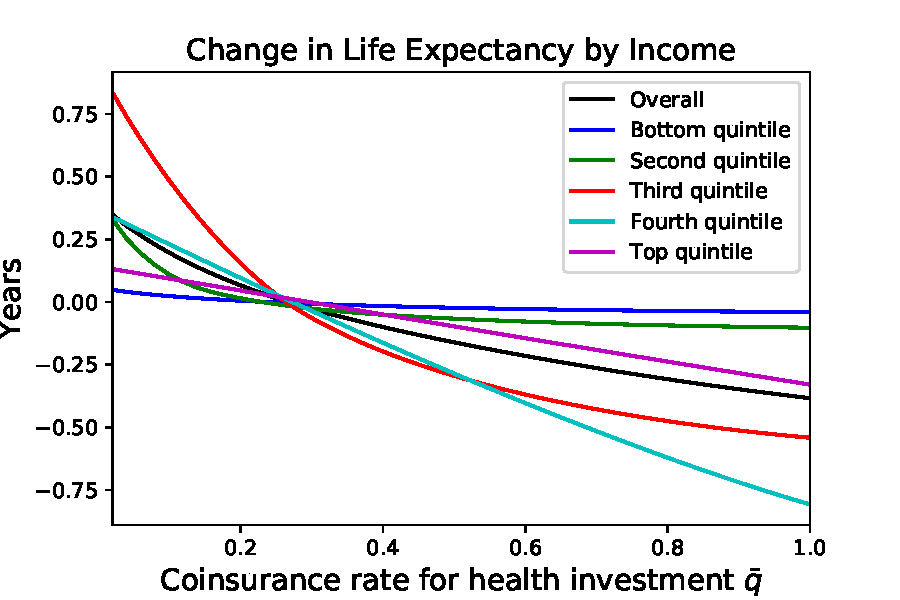
\includegraphics[width=\textwidth]{../Figures/FlatCopayInvstLifeExp.pdf}
        \caption{Change in life expectancy}
    \end{subfigure}
    \begin{subfigure}[b]{0.49\textwidth}
        \centering
        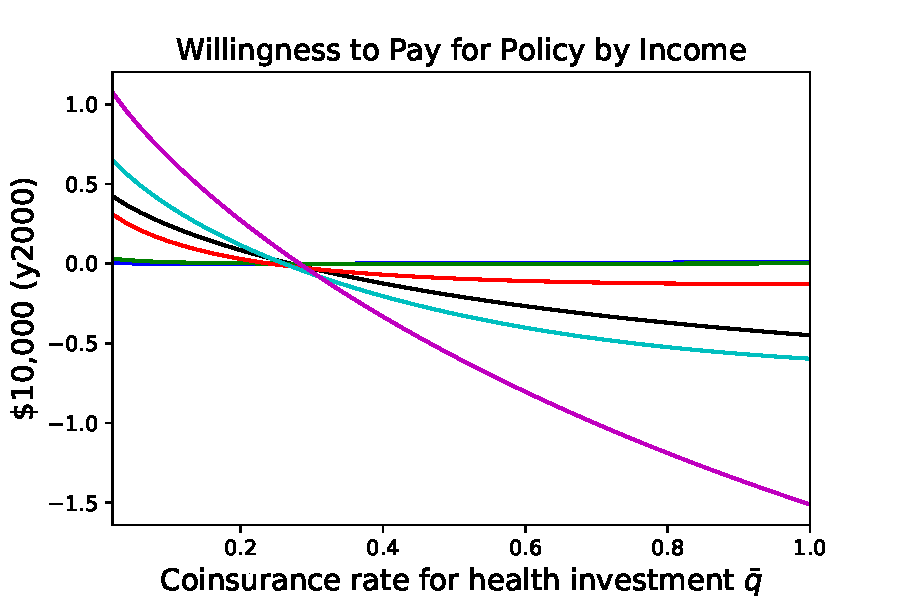
\includegraphics[width=\textwidth]{../Figures/FlatCopayInvstWTP.pdf}
        \caption{Willingness to pay for policy}
    \end{subfigure}
    \caption{Counterfactual experiment: Universal coinsurance rate for health investment}
    \label{fig:FlatCopayInvst}
\end{figure}

\newpage


\begin{figure}[h!]
    \centering
    \begin{subfigure}[b]{0.49\textwidth}
        \centering
        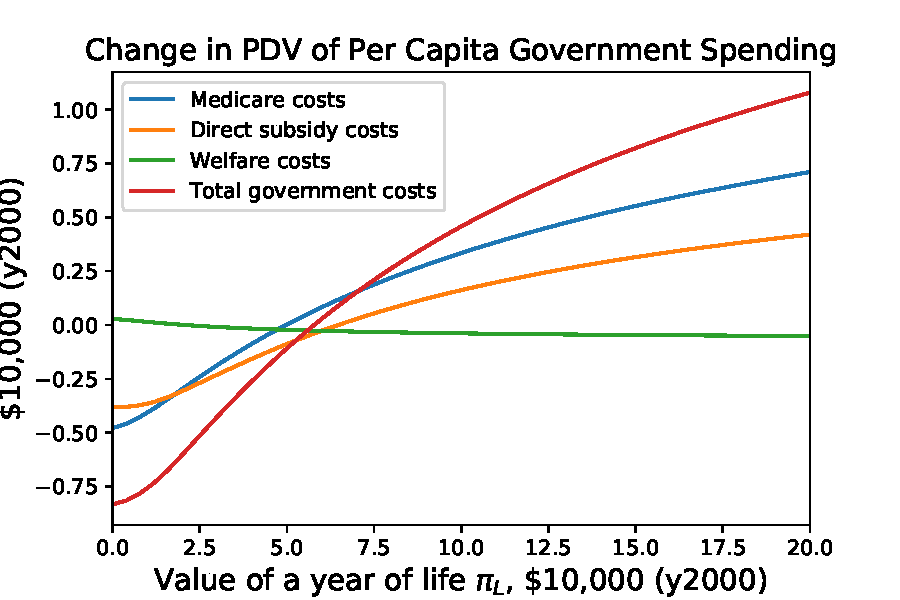
\includegraphics[width=\textwidth]{../Figures/SocOptByLifePriceGovtChange.pdf}
        \caption{Change in government expenditures}
    \end{subfigure}
    \begin{subfigure}[b]{0.49\textwidth}
        \centering
        \includegraphics[width=\textwidth]{../Figures/SocOptByLifePriceMedChange.pdf}
        \caption{Change in composition of medical spending}
    \end{subfigure}
    \begin{subfigure}[b]{0.49\textwidth}
        \centering
        \includegraphics[width=\textwidth]{../Figures/SocOptByLifePriceGovtChangeByInc.pdf}
        \caption{Change in government spending by income}
    \end{subfigure}
    \begin{subfigure}[b]{0.49\textwidth}
        \centering
        \includegraphics[width=\textwidth]{../Figures/SocOptByLifePriceOOPchangeByInc.pdf}
        \caption{Change in out-of-pocket expenses by income}
    \end{subfigure}
    \begin{subfigure}[b]{0.49\textwidth}
        \centering
        \includegraphics[width=\textwidth]{../Figures/SocOptByLifePriceLifeExp.pdf}
        \caption{Change in life expectancy}
    \end{subfigure}
    \begin{subfigure}[b]{0.49\textwidth}
        \centering
        \includegraphics[width=\textwidth]{../Figures/SocOptByLifePriceWTP.pdf}
        \caption{Willingness to pay for policy}
    \end{subfigure}
    \caption{Counterfactual experiment: ``Socially optimal'' subsidy for health investment, by value placed on a year of life}
    \label{fig:SocOptByLifePrice}
\end{figure}


\clearpage


\begin{figure}[h!]
    \centering
    \begin{subfigure}[b]{0.49\textwidth}
        \centering
        \includegraphics[width=\textwidth]{../Figures/SocOpt57CopayWomen65.pdf}
        \caption{Women, age 65}
    \end{subfigure}
    \begin{subfigure}[b]{0.49\textwidth}
        \centering
        \includegraphics[width=\textwidth]{../Figures/SocOpt57CopayMen65.pdf}
        \caption{Men, age 65}
    \end{subfigure}
    \begin{subfigure}[b]{0.49\textwidth}
        \centering
        \includegraphics[width=\textwidth]{../Figures/SocOpt57CopayWomen75.pdf}
        \caption{Women, age 75}
    \end{subfigure}
    \begin{subfigure}[b]{0.49\textwidth}
        \centering
        \includegraphics[width=\textwidth]{../Figures/SocOpt57CopayMen75.pdf}
        \caption{Men, age 75}
    \end{subfigure}
    \begin{subfigure}[b]{0.49\textwidth}
        \centering
        \includegraphics[width=\textwidth]{../Figures/SocOpt57CopayWomen85.pdf}
        \caption{Women, age 85}
    \end{subfigure}
    \begin{subfigure}[b]{0.49\textwidth}
        \centering
        \includegraphics[width=\textwidth]{../Figures/SocOpt57CopayMen85.pdf}
        \caption{Men, age 85}
    \end{subfigure}
    \caption{Coinsurance rates for baseline Medicare policy (dashed) and ``socially optimal'' health investment subsidy policy (solid) when the government's objective is to maximize years of life less total medical costs, valuing a year of life at \$57,500.}
    \label{fig:SocOpt57Copay}
\end{figure}


\clearpage


\begin{figure}[h!]
    \centering
    \begin{subfigure}[b]{0.49\textwidth}
        \centering
        \includegraphics[width=\textwidth]{../Figures/SocOpt00CopayWomen65.pdf}
        \caption{Women, age 65}
    \end{subfigure}
    \begin{subfigure}[b]{0.49\textwidth}
        \centering
        \includegraphics[width=\textwidth]{../Figures/SocOpt00CopayMen65.pdf}
        \caption{Men, age 65}
    \end{subfigure}
    \begin{subfigure}[b]{0.49\textwidth}
        \centering
        \includegraphics[width=\textwidth]{../Figures/SocOpt00CopayWomen75.pdf}
        \caption{Women, age 75}
    \end{subfigure}
    \begin{subfigure}[b]{0.49\textwidth}
        \centering
        \includegraphics[width=\textwidth]{../Figures/SocOpt00CopayMen75.pdf}
        \caption{Men, age 75}
    \end{subfigure}
    \begin{subfigure}[b]{0.49\textwidth}
        \centering
        \includegraphics[width=\textwidth]{../Figures/SocOpt00CopayWomen85.pdf}
        \caption{Women, age 85}
    \end{subfigure}
    \begin{subfigure}[b]{0.49\textwidth}
        \centering
        \includegraphics[width=\textwidth]{../Figures/SocOpt00CopayMen85.pdf}
        \caption{Men, age 85}
    \end{subfigure}
    \caption{Coinsurance rates for baseline Medicare policy (dashed) and ``socially optimal'' health investment subsidy policy (solid) when the government's objective is to minimize total medical costs, ignoring longevity.}
    \label{fig:SocOpt00Copay}
\end{figure}


\clearpage




\begin{figure}[h!]
    \centering
    \begin{subfigure}[b]{0.45\textwidth}
        \centering
        \includegraphics[width=\textwidth]{../Figures/PreventiveSubCostPerYear.pdf}
        \caption{Preventive care voucher}
    \end{subfigure}
    \begin{subfigure}[b]{0.45\textwidth}
        \centering
        \includegraphics[width=\textwidth]{../Figures/CurativeSubCostPerYear.pdf}
        \caption{Curative care voucher}
    \end{subfigure}
    \begin{subfigure}[b]{0.45\textwidth}
        \centering
        \includegraphics[width=\textwidth]{../Figures/FlatCopayInvstCostPerYearZoom.pdf}
        \caption{Universal coinsurance rate}
    \end{subfigure}
    \begin{subfigure}[b]{0.45\textwidth}
        \centering
        \includegraphics[width=\textwidth]{../Figures/SocOptByLifePriceCostPerYear.pdf}
        \caption{``Socially optimal'' insurance}
    \end{subfigure}
    \caption{Government cost per year of life added across alternative health investment subsidy policies.  Each panel divides government cost curves in panel (c) by corresponding change in life expectancy curves in panel (e) from Figures \ref{fig:PreventiveSub}-\ref{fig:SocOptByLifePrice}.}
    \label{fig:CostPerYear}
\end{figure}


\begin{figure}[h!]
	\centering
	\begin{subfigure}[b]{0.45\textwidth}
		\centering
		\includegraphics[width=\textwidth]{../Figures/HealthCoeffByIncWealthOnly7a.pdf}
		\caption{Health coefficients}
	\end{subfigure}
	\begin{subfigure}[b]{0.45\textwidth}
		\centering
		\includegraphics[width=\textwidth]{../Figures/OOPcoeffByIncWealthOnly7a.pdf}
		\caption{OOP coefficients}
	\end{subfigure}
	\caption{Coefficients on income-wealth quintiles in regressions on health transitions and out-of-pocket medical spending in HRS data (dots) vs estimated model (lines) when the estimation \textit{only} tries to fit moment category 7(a).}
	\label{fig:MomentCat7X}
\end{figure}


\newpage


\begin{figure}[h!]
    \centering
    \begin{subfigure}[b]{0.49\textwidth}
        \centering
        \includegraphics[width=\textwidth]{../Figures/TotalMedPDVbyIncomeWomen.pdf}
        \caption{Total medical expenses, women}
    \end{subfigure}
    \begin{subfigure}[b]{0.49\textwidth}
        \centering
        \includegraphics[width=\textwidth]{../Figures/TotalMedPDVbyIncomeMen.pdf}
        \caption{Total medical expenses, men}
    \end{subfigure}
    \begin{subfigure}[b]{0.49\textwidth}
        \centering
        \includegraphics[width=\textwidth]{../Figures/OOPmedPDVbyIncomeWomen.pdf}
        \caption{Out-of-pocket medical expenses, women}
    \end{subfigure}
    \begin{subfigure}[b]{0.49\textwidth}
        \centering
        \includegraphics[width=\textwidth]{../Figures/OOPmedPDVbyIncomeMen.pdf}
        \caption{Out-of-pocket medical expenses, men}
    \end{subfigure}
    \caption{PDV of total and out-of-pocket medical expenditures at age 69 ($\Age=2$) by sex, health, and income; calculated at median wealth for each type}
    \label{fig:MedPDV}
\end{figure}


\begin{figure}[h!]
    \centering
    \begin{subfigure}[b]{0.49\textwidth}
        \centering
        \includegraphics[width=\textwidth]{../Figures/LifeExpectancyByIncomeWomen.pdf}
        \caption{Women}
    \end{subfigure}
    \begin{subfigure}[b]{0.49\textwidth}
        \centering
        \includegraphics[width=\textwidth]{../Figures/LifeExpectancyByIncomeMen.pdf}
        \caption{Men}
    \end{subfigure}
    \caption{Remaining life expectancy at age 69 ($\Age=2$) by sex, health, and income; calculated at median wealth for each type}
    \label{fig:LifeExpectancy}
\end{figure}



\clearpage

\appendix
\section*{Appendices}

\section{Solution}
\label{app:Solution}

Summarize logic of EGM. The general logic of EGM is straightforward:
\begin{enumerate}
\item Assuming that the agent is \textit{ending} the period in a particular state, what controls must he have chosen at the \textit{beginning} of the period for this to \textit{have been} optimal?

\item If the agent ends the period in that state, and chose those controls, from what state must he have taken such an action?
\end{enumerate}
To solve the model by EGM, we assume some end-of-period state $(\Assets_{it},\PostHealth_{it})$ has been reached and solve for the controls that would justify it, then invert the budget constraint (or other transition equation) to find the corresponding decision-time state $(\Bank_{it},\Health_{it},\MedShk_{it})$.  When solving the model, the $\MedShk_{it}$ state is replaced with the ``medical need shock deviation'' $\zeta_{it}$, representing standard deviations from the mean log medical need shock.

The general solution method for the age $\Age$ problem of type $\Type$ can be summarized as:
\begin{enumerate}
\item Specify exogenous grids of end-of-period states $\mathbb{A}_{\Type \Age}$ and $\overline{\mathbb{H}}_{\Type \Age}$.

\item Specify an exogenous grid of log medical need shock deviations $\zeta_{it} \in \mathbb{Z}_{\Type \Age}$.

\item Compute $\PostValue_{\Type \Age}(\Assets,\PostHealth)$ and its first derivatives on $\mathbb{A}_{\Type \Age} \times \overline{\mathbb{H}}_{\Type \Age}$.

\item Use the first order condition for consumption $\eqref{OPTc}$ to find $\Con_{it}$ for all points in $\mathbb{A}_{\Type \Age} \times \overline{\mathbb{H}}_{\Type \Age}$.

\item Use the first order condition for medical consumption $\eqref{OPTm}$ to find $\Con_{it}$ for all points in $\mathbb{A}_{\Type \Age} \times \overline{\mathbb{H}}_{\Type \Age} \times \mathbb{Z}_{\Type \Age}$.

\item Use the procedure in Appendix \ref{app:OPTn} to solve for $\Invst_{it}$ and endogenous $\Health_{it}$ for all points in $\mathbb{A}_{\Type \Age} \times \overline{\mathbb{H}}_{\Type \Age}$.

\item Use \eqref{BudgetEGM} to calculate endogenous $\Bank_{it}$ gridpoints from which these controls were chosen.

\item Use the procedure in Appendix \ref{app:LiqCnstSolution} to generate controls and endogenous gridpoints for liquidity constrained solutions.

\item Concatenate the interior solutions and corresponding liquidity constrained solutions.

\item Use the G2EGM procedure in Appendix \ref{app:G2EGM} to ``reinterpolate'' 3D simplices formed by the endogenous gridpoints onto exogenous dense grids of $\Bank_{it}$, $\Health_{it}$, and $\zeta_{it}$.

\item Construct interpolations of investment and ``expenditure'' (see Appendix \ref{app:ConFloorSolution}) from the outputs of the G2EGM step.

\item For each $(\Bank_{it},\Health_{it})$, use the procedure in Appendix \ref{app:ConFloorSolution} to find the critical medical need shock above which the individual will use the consumption floor.

\item Integrate value and marginal value of $\Bank_{it}$ (and possibly other objects) across the distribution of $\zeta_{it}$ using the procedure in Appendix \ref{app:Integration}.

\item Construct interpolated representations of the value and marginal value functions.
\end{enumerate}


\subsection{Solving for Optimal Investment}
\label{app:OPTn}

The solution for optimal health investment in \eqref{OPTn} assumed an interior solution ($\Invst_{it} > 0$, $\Assets_{it} \geq 0$) and elided the fact that the coinsurance rate $\Copay_{it}$ appears on the RHS and depends on $\Health_{it}$, which is not known from the perspective of the end of the period when using the endogenous grid method.  To solve for optimal $\Invst_{it}$ from any given end-of-period state $(\Assets_{it},\PostHealth_{it})$ for which end-of-period marginal values have been computed, the following procedure is used:
\begin{enumerate}
\item Begin with an initial guess of $\Invst_{it}=0$.

\item Use the quadratic formula to solve \eqref{PostHealth} for the unique $\Health_{it} \in [0,1]$ at current guess of $\Invst_{it}$.

\item Calculate $\Copay_{it} = \CopayFunc_{\Type \Age}(\Health_{it})$, then compute the RHS of \eqref{OPTn} to update the guess of $\Invst_{it}$.

\item If the updated $\Invst_{it}$ is complex (because $\PostValue^\PostHealth_{\Type \Age}(\Assets_{it},\PostHealth_{it}) < 0$) or negative, replace $\Invst_{it} = 0$.

\item Calculate the absolute change in $\Invst_{it}$ between new and previous guess.  If less than $10^{-6}$, STOP; else go to step 2.
\end{enumerate}

In step 4, the agent would only end the period in this way while acting optimally if the optimal choice were to purchase no health investment; the fixed point loop thus accounts for the possibility of a solution that is constrained by $\Invst_{it} \geq 0$.  The inversion from end-of-period health $\PostHealth_{it}$ and investment $\Invst_{it}$ to beginning-of-period health $\Health_{it}$ has a unique closed form solution on the unit interval (i.e.\ the set of valid $\Health_{it}$ values) as long as $\HealthParam_{\Age 1}$ and $\HealthParam_{\Age 2}$ are non-negative (as is the case with the estimated parameters) or $\frac{\HealthParam_{\Age 1}}{\HealthParam_{\Age 2}} < -2$ if $\HealthParam_{\Age 2} < 0$ so that the negative curvature is small relative to the linear term.  The health production function $\HealthProdFunc$ was assumed to have a monotonic form, and thus is invertible.


\subsection{Liquidity Constrained Solution}
\label{app:LiqCnstSolution}

When an individual is liquidity constrained and ends the period with $\Assets_{it}=0$, the first order conditions for an interior solution in the controls do not generally apply; rather, the individual would prefer to spend more on some good and borrow against future income, but this is not permitted.  Instead, a liquidity-constrained individual uses only the first order conditions \textit{among} consumption, medical consumption and health investment-- that the marginal value of a dollar spent on any of the goods is equal.  Equating the marginal value of consumption and medical consumption is expressed in \eqref{OPTm}, while the first order condition between consumption and health investment is:
\begin{equation}\label{OPTnCnst}
\Con_{it}^{-\CRRAcon} = \HealthProdFunc^\Invst(\Invst_{it}) \PostValue^\PostHealth_{\Type \Age}(0,\PostHealth_{it})/\Copay_{it} \Longrightarrow \Invst_{it} = \left( \frac{\Copay_{it} \Con_{it}^{-\CRRAcon}}{\HealthProdParam_1 \HealthProdParam_2 \PostValue_{\iota j}^\PostHealth(0,\PostHealth_{it})} \right)^{1/(\HealthProdParam_2 - 1)} - \HealthProdParam_0.
\end{equation}

The end-of-period marginal value of post-health when $\Assets_{it}=0$ was already computed as part of the interior solution, as $\Assets_{it}=0 \in \mathbb{A}_{\Type \Age}$.  To solve for \textit{liquidity constrained} solutions associated with this end-of-period state, I exploit the fact that the individual's combined spending on consumption and medical consumption $\Xpend_{it}$ must be \textit{less} than the $\Xpend_{it}$ associated with the interior solution for the same end-of-period state.  For a particular end-of-period state $(0,\PostHealth_{it})$ and medical need shock $\MedShk_{it}$ in the grid, define $\overline{\Xpend}_{it} = \Con_{it} + \Copay_{it} \Care_{it}$ for the interior solution, and define a uniform grid of $\Xpend_{it}$ values on $[0,\overline{\Xpend}_{it}]$ labeled $\mathbb{X}$; I used a grid with 16 points.  The liquidity constrained solution in which the individual spends $\Xpend_{it} \in \mathbb{X}$ on consumption and medical consumption and ends the period at $(0,\PostHealth_{it})$ can be found with the following fixed point procedure:
\begin{enumerate}
\item Use the first order condition between $\Con$ and $\Care$ to find $\Con_{it}$ and $\Care_{it}$ (see Appendix \ref{app:ConFloorSolution}).

\item Begin with an initial guess of $\Health_{it} = \overline{\Health}_{it}$, the endogenous gridpoint for the interior solution at $(0,\PostHealth_{it})$.

\item Calculate $\Copay_{it} = \CopayFunc_{\Type \Age}(\Health_{it})$, then compute the RHS of \eqref{OPTnCnst} get a guess of $\Invst_{it}$.

\item If $\Invst_{it}$ is complex (because $\PostValue^\PostHealth_{\Type \Age}(0,\PostHealth_{it}) < 0$) or negative, replace $\Invst_{it} = 0$.

\item Use the quadratic formula to solve \eqref{PostHealth} for the unique $\Health_{it} \in [0,1]$ at current guess of $\Invst_{it}$.

\item Calculate the absolute change in $\Health_{it}$ between new and previous guess.  If less than $10^{-5}$, go to step 7; else go to step 2.

\item Calculate the endogenous gridpoint in bank balances $\Bank_{it} = \Xpend_{it} + \Copay_{it} \Invst_{it} + \Premium_{it}$.
\end{enumerate}
When repeated across all of the values in $\mathbb{X}$, this yields a set of endogenous gridpoints $(\Bank_{it},\Health_{it},\MedShk_{it})$ and liquidity constrained controls $(\Con_{it},\Care_{it},\Invst_{it},0)$ associated with a particular end-of-period state.


\subsection{Consumption Floor Solution}
\label{app:ConFloorSolution}

Retirees in the model have the option of using the consumption floor, yielding quantities of the goods given in \eqref{ConFloor}.  To accurately solve the problem, we want to know for any values of $(\Bank_{it},\Health_{it})$ what is the \textit{critical shock} $\MedShk^*$ at which the individual uses the consumption floor if $\MedShk_{it}$ is at least as great.  This will allow for a more accurate numeric integration across medical need shocks and reduce some numeric difficulties.

To find the critical shock, begin by considering the first order conditon between consumption and medical consumption, given in \eqref{OPTm}.  Suppose the individual faces some medical need shock $\MedShk_{it}$ and coinsurance rate $\Copay_{it}$ and is going to spend a total of $\Xpend_{it}$ out-of-pocket on consumption and medical consumption.  Let $(\Con_{it},\Care_{it})$ be the solution to \eqref{OPTm} and implicitly define $\chi \in \R$ by:
\begin{equation}\label{Xpend}
\Con_{it} = \frac{\Xpend_{it}}{1 + \exp(-\chi)}, \qquad \Copay_{it} \Care_{it} = \frac{\exp(-\chi)\Xpend_{it}}{1 + \exp(-\chi)}.
\end{equation}
Thus $\chi$ represents a transformation of the share of e\textit{X}penditure that is used for consumption (with complementary share spent on out-of-pocket medical expenses).  Substituting these expressions into \eqref{OPTm}, we get:
\begin{equation}
\Copay_{it}^{-1} \frac{\exp(-\chi)\Xpend_{it}}{1 + \exp(-\chi)} = \Copay_{it}^{-1/\CRRAcare} \MedShk_{it}^{1-1/\CRRAcare} \left(\frac{\Xpend_{it}}{1 + \exp(-\chi)} \right)^{\CRRAcon/\CRRAcare}.
\end{equation}
Moving the leading factor to the RHS and taking logs:
\begin{equation*}
-\chi - \log(1 + \exp(-\chi)) + \log \Xpend_{it} = \left(1-\frac{1}{\CRRAcare}\right) \log(\Copay_{it} \MedShk_{it}) + \frac{\CRRAcon}{\CRRAcare} \log \Xpend_{it} - \frac{\CRRAcon}{\CRRAcare} \log(1 + \exp(-\chi)) \Longrightarrow
\end{equation*}
\begin{equation}\label{AlephBeth}
\underbrace{\left(1-\frac{\CRRAcon}{\CRRAcare}\right) \log \Xpend_{it} - \left(1-\frac{1}{\CRRAcare}\right) \log(\Copay_{it} \MedShk_{it})}_{\equiv \beth(\Xpend_{it}, \Copay_{it} \MedShk_{it})} = 
\underbrace{\chi + \left(1-\frac{\CRRAcon}{\CRRAcare}\right) \log(1 + \exp(-\chi))}_{\equiv \aleph(\chi)}.
\end{equation}
Assuming that $\rho < \nu$, $\aleph(b)$ is strictly increasing, with derivative:
\begin{equation}
\aleph'(\chi) = 1 - \left(1-\frac{\CRRAcon}{\CRRAcare}\right)  \frac{\exp(-\chi)}{1 + \exp(-\chi)} > 0.
\end{equation}
Further note that $\aleph$ is linear in the limit in both directions:
\begin{equation}
\lim_{\chi \rightarrow -\infty} \aleph(\chi) = \frac{\CRRAcon}{\CRRAcare} \chi, \qquad \lim_{\chi \rightarrow \infty} \aleph(\chi) = \chi.
\end{equation}
In fact, nearly all of the curvature of $\aleph$ occurs near $\chi=0$, roughly in the range $[-10,10]$.  Thus $\aleph(\chi)$ is well approximated by a cubic spline interpolation using a grid of $\chi$ values that is dense near zero and increasingly sparse as $|\chi|$ becomes large, with linear extrapolation.  Likewise, the inverse function $\aleph^{-1}$ exists and is also well represented by a cubic spline interpolation.  We can thus define a function that yields $\chi$ as a function of $\Xpend_{it}$ and $\Copay_{it} \MedShk_{it}$:
\begin{equation}\label{OptCshare}
\hat{\chi}(\Xpend_{it}, \Copay_{it} \MedShk_{it}) = \aleph^{-1}(\beth(\Xpend_{it}, \Copay_{it} \MedShk_{it}).
\end{equation}
To construct a very accurate representation of $\aleph^{-1}$:
\begin{enumerate}
\item Specify a grid of $\chi$ values called $\mathbb{K}$ that is dense near zero.  I used a double-exponential grid between 0 and 30, plus its mirror image down to -30.

\item Evaluate $\mathbb{G} = \aleph(\mathbb{K})$ and $\mathbb{D} = \aleph'(\mathbb{K})^{-1}$.

\item Construct a cubic interpolation with gridpoints $\mathbb{G}$, function values $\mathbb{K}$, and slopes $\mathbb{D}$.
\end{enumerate}

This transformation is used when solving for interior and liquidity constrained solutions and representing the policy function.  Rather than separately constructing interpolated consumption and medical consumption functions, I instead calculate $\Xpend_{it} = \Con_{it} + \Copay_{it} \Care_{it}$ and interpolate the ``expenditure'' function over the endogenous gridpoints.  Actual consumption and medical consumption are recovered during simulation by using $\chi^*$.

This transformation can also be used to find the critical shock $\MedShk^*$ above which the individual will use the consumption floor.  Suppose the individual has bank balances of $\Bank_{it}$ and is spending all of it on $\Con_{it}$ and $\Care_{it}$ because $\MedShk_{it}$ is very large (so $\Xpend_{it} = \Bank_{it}$).  How large must $\MedShk_{it}$ be for the individual to consume at the floor?  Substituting  $\Con_{it} = \ConFloor$ and $\Xpend_{it} = \Bank_{it}$ into the first half of \eqref{Xpend} and solving for $\chi$, we get:\footnote{When $\Bank_{it} < \ConFloor$, the retiree requires welfare assistance at any medical need shock.}
\begin{equation}
\chi = -\log \left( \frac{\Bank_{it}}{\ConFloor} - 1 \right).
\end{equation}
Substituting this expression for $\chi$ into \eqref{AlephBeth}, along with $\Xpend_{it} = \Bank_{it}$ and solving for $\MedShk_{it}$ yields:
\begin{equation}
\MedShk^* = \exp \left( \frac{\CRRAcare - \CRRAcon}{\CRRAcare - 1} \log \ConFloor + \frac{\CRRAcare}{\CRRAcare - 1} \log \left( \frac{\Bank_{it}}{\ConFloor} - 1 \right) - \log \Copay_{it} \right).
\end{equation}

This closed form solution for the critical medical need shock is valid as long as the individual is liquidity constrained \textit{and} non-negative health investment constrained for medical need shocks just below the critical shock.  That is, there is no state $(\Bank_{it},\Health_{it},\MedShk_{it})$ at which it is optimal to end the period with $\Assets_{it} > 0$ for $\MedShk_{it}$ but use the consumption floor for $\MedShk_{it} + \epsilon$; nor any state at which it is optimal to buy $\Invst_{it} > 0$  for $\MedShk_{it}$ but use the consumption floor for $\MedShk_{it} + \epsilon$.  The first possibility is ruled out because of the first order and envelope conditions: Optimal (interior) consumption equates marginal utility of consumption today to expected marginal utility of consumption in the next period (plus the marginal bequest motive); because next period's consumption is never less than the consumption floor, optimal interior consumption is strictly greater than the consumption floor.  The second possibility depends on the parameter values of $\LifeUtility$, $\ConFloor$, $\CRRAcon$, and $\HealthProdParam$, but never happens at any ``reasonable'' parameters that are not immediately ruled out by the data.


\subsection{G2EGM: Reinterpolation}
\label{app:G2EGM}

The grid of end-of-period assets $\mathbb{A}_{\Type \Age}$ is specified as a 48 point array, triple-exponentially spaced between zero and $100 \cdot \Inc_{\Type \Age}$; the grid of end-of-period health $\overline{\mathbb{H}}_{\Type \Age}$ is specified as a uniformly spaced 20 point array.  The minimum value of $\overline{\mathbb{H}}_{\Type \Age}$ corresponds to the $\PostHealth_{it}$ value that would be attained from $\Health_{it} = 0$ with no health investment, and the maximum value is the $\PostHealth_{it}$ that would be reached from $\Health_{it} = 1$ and \$1 million of health investment ($\Invst_{it} = 100$).  Thus the grid of end-of-period states spans the set of situations that retirees could reasonably encounter.\footnote{To the extent that extrapolation is ever required for very rich retirees, the policy functions are very linear at high values of $\Bank_{it}$}

While the grid of end-of-period states is rectilinear, the set of endogenous gridpoints generated by EGM in a model with multiple endogenous state variables is \textit{irregular}.  While it is possible to construct interpolated functions on irregular data, as in \cite{ludwig18} and \cite{white15}, the endogeneity of health and mortality and this model create the possibility that there are non-concave regions of the value function.  Depending on the extent of the non-concavities (and risk faced by agents), the set of first-order-condition-satisfying endogenous gridpoint generated by EGM can ``double back'' on itself, so that some states have \textit{multiple} candidate solutions.

To deal with the possibility of multiple solutions to the optimality conditions at some states, I employ \cite{jorgensen17}'s G2EGM method, a generalization of \cite{fella14} for models with multiple endogenous states.  The essence of G2EGM is to ``reinterpolate'' the irregular set of endogenous gridpoints onto an exongenously specified dense grid of decision-time states, using barycentric weights over simplices of ``adjacent'' endogenous gridpoints.\footnote{The simplices come from ``adjacent'' endogenous gridpoints in the sense that they were generated from adjacent gridpoints in the end-of-period state grid.}  If some decision-time state $(\Bank_{it},\Health_{it},\MedShk_{it})$ has multiple candidate solutions, the G2EGM procedure considers them sequentially and only keeps the one with the highest value-- the true optimal controls.

For the G2EGM ``reinterpolation'' step, I specify the grid of bank balances $\mathbb{B}_{\Type \Age}$ as a 96 point array, triple exponentially spaced between $\Inc_{\Type \Age}$ and $100 \cdot \Inc_{\Type \Age}$, and the grid of health $\mathbb{H}_{\Type \Age}$ as a uniformly spaced 40 point grid on $[0,1]$ (the full range of $\Health_{it}$).  The grid of medical need shocks is expressed as a uniformly spaced 73 point grid on $\zeta_{it}$ between -3 and 5.


\subsection{Integration Across $\MedShk$}
\label{app:Integration}

The final step in the solution method each period is to integrate $\Value_{\Type \Age}(\Bank_{it},\Health_{it},\MedShk_{it})$ and $\Value^\Bank_{\Type \Age}(\Bank_{it},\Health_{it},\MedShk_{it})$ with respect to the distribution of $\MedShk_{it}$ to generate \textit{expected} value and marginal value functions $\overline{\Value}_{\Type \Age}(\Bank_{it},\Health_{it})$ and $\overline{\Value}^\Bank_{\Type \Age}(\Bank_{it},\Health_{it},\MedShk_{it})$ from a moment in time \textit{just before} the medical need shock is drawn.  During counterfactual exercises, several other objects of interest are also calculated using the same method.  This appendix describes the numeric method used to integrate across $\MedShk_{it}$ and the accounting procedures used to calculate the present discounted value of various objects.

For each $(\Bank_{it},\Health_{it}) \in \mathbb{B}_{\Type \Age} \times \mathbb{H}_{\Type \Age}$, the following steps are used to integrate over $\MedShk_{it}$:
\begin{enumerate}
\item Specify a temporary grid of $\zeta_{it}$ uniformly distributed between $-3$ and $\zeta^*$ for this $(\Bank_{it},\Health_{it})$; I used a 73 point grid, three times as dense as the original $\mathbb{Z}$.  If $\zeta^* > 5$, this $(\Bank_{it},\Health_{it})$ is labeled as ``never at consumption floor'' and the top of the grid is set at 5; if $\zeta^* < -3$, this $(\Bank_{it},\Health_{it})$ is labeled as ``always at consumption floor''.

\item If this point is ``always'' at the consumption floor, go to step 5.

\item Calculate the probability of being at the consumption floor as $\Phi(\zeta^*)$.

\item Calculate the probability of being at each of the temporary $\zeta_{it}$ gridpoints as:
\begin{equation}
\Prob[\zeta = \zeta_{it}] = (1 - \Phi(\zeta^*)) \cdot \frac{\phi(\zeta_{it})} {\sum \phi(\overline{\mathbb{Z}})}
\end{equation}

\item Calculate expected value conditional on exceeding the critical shock using the truncated lognormal formula:
\begin{equation*}
\tilde{\mu}_{it}  = \left(1 - \frac{1}{\CRRAcare}\right) \mu_{it}, \qquad \tilde{\sigma}_{it} = \left(1 - \frac{1}{\CRRAcare}\right) \sigma_{it},
\end{equation*}
\begin{equation}
\E [\MedShk_{it}^{1-1/\CRRAcare} | \MedShk_{it} > \MedShk^*] = \frac{1}{2} \exp(\tilde{\mu}_{it}+0.5 \sigma_{it}^2) \cdot \left( \erf \left( \sqrt{0.5}(\tilde{\sigma}_{it}-\zeta^*) \right) + 1 \right) / \Phi(\zeta^*),
\end{equation}
\end{enumerate}
\begin{equation*}
\E [\Value_{\Type \Age}(\Bank_{it},\Health_{it},\MedShk_{it}) | \MedShk_{it} > \MedShk^* ] = \frac{\ConFloor^{1-\CRRAcon}}{1-\CRRAcon} + \E [\MedShk_{it}^{1-1/\CRRAcare} | \MedShk_{it} > \MedShk^*] \cdot \frac{\Copay_{it}^{1- 1/\CRRAcare} \ConFloor^{\CRRAcon/\CRRAcare - \CRRAcon}}{1 - \CRRAcare} - \frac{\LifeUtility^{1-\CRRAcon}}{1-\CRRAcon} + \PostValue_{\Type \Age}(0,\PostHealth_{it} | \Invst_{it}=0).
\end{equation*}

\begin{enumerate}
\setcounter{enumi}{6}

\item Calculate overall expected value as:
\begin{equation}
\overline{\Value}_{\Type \Age}(\Bank_{it},\Health_{it}) = \Phi(\zeta^*) \E [\Value_{\Type \Age}(\Bank_{it},\Health_{it},\MedShk_{it}) | \MedShk_{it} > \MedShk^* ] + \sum_{\zeta_{it} \in \overline{\mathbb{Z}}} \Prob[\zeta = \zeta_{it}] \Value_{\Type \Age}(\Bank_{it},\Health_{it},\MedShk_{it}).
\end{equation}

\item Use the envelope condition and the policy function to calculate the marginal value of bank balances as $\Value_{\Type \Age}^\Bank(\Bank_{it},\Health_{it},\MedShk_{it}) = \Con_{it}^{-\CRRAcon}$ for $\MedShk_{it} = \exp(\mu_{it} + \sigma_{it}\zeta_{it})$ on $\overline{\mathbb{Z}}$.

\item Calculate overall expected marginal value of bank balances as:
\begin{equation}
\overline{\Value}^\Bank_{\Type \Age}(\Bank_{it},\Health_{it}) = \sum_{\zeta_{it} \in \overline{\mathbb{Z}}} \Prob[\zeta = \zeta_{it}] \Value_{\Type \Age}^\Bank(\Bank_{it},\Health_{it},\MedShk_{it}).
\end{equation}
\end{enumerate}
The arrays of beginning-of-period value and marginal value are then used to construct interpolated representations of these functions on $\mathbb{B}_{\Type \Age} \times \mathbb{H}_{\Type \Age}$.

During the counterfactual experiments, the present discounted value of various quantities are calculated as a function of the agent's beginning-of-period state $(\Bank_{it},\Health_{it})$ just before the medical need shock $\MedShk_{it}$ is drawn.  The accounting of expenses when the individual does \textit{not} use the consumption floor are:
\begin{equation}
TotalMed_{it} = \Care_{it} + \Invst_{it}, \qquad OOPmed_{it} = \OOP_{it} =  (\Care_{it} + \Invst_{it})\cdot \Copay_{it} - \Subsidy_{\Type \Age}(\Health_{it},\Invst_{it}),
\end{equation}
\begin{equation*}
Welfare_{it} = 0, \qquad Medicare_{it} = (\Care_{it} + \Invst_{it})\cdot(1-\Copay_{it}), \qquad Subsidy_{it} = \Subsidy_{\Type \Age}(\Health_{it},\Invst_{it}).
\end{equation*}
When the individual uses the consumption floor, the following accounting identities are used (note that $\Invst_{it}=0$ when an individual uses the consumption floor):
\begin{equation}
TotalMed_{it} = \Care_{it}, \qquad OOPmed_{it} = \OOP_{it} =  \max(\Bank_{it} - \Premium_{it} - \ConFloor, 0),
\end{equation}
\begin{equation*}
Welfare_{it} = \ConFloor + \Premium_{it} + \Care_{it} - \Bank_{it} - Medicare_{it}, \qquad Medicare_{it} = (1 - \Copay_{it}) \OOP_{it}/\Copay_{it}, \qquad Subsidy_{it} = 0.
\end{equation*}
When accounting for medical expenses, it is assumed that the retiree prioritizes paying for consumption and insurance premiums, and any remaining resources go toward medical expenses.  Further, I assume that medical expenses that were paid partly out of pocket by the individual are covered in remainder by Medicare; all expenses \textit{not} accounted for by the individual's $\Bank_{it}$ or Medicare payments are deemed to be ``welfare''.  Note that whether or not the individual uses the consumption floor, the sum of out-of-pocket expenses, Medicare, welfare, and the subsidy always equals total medical expenses as an accounting identity.\footnote{This could be violated if $\Bank_{it} - \Premium_{it} - \ConFloor < 0$ so that the retiree needs welfare just to pay the consumption floor, let alone medical care.}

The expectation of medical consumption conditional on hitting the consumption floor is:
\begin{equation}
\E [\Care_{it} | \MedShk_{it} > \MedShk^*] = \E [\MedShk_{it}^{1-1/\CRRAcare} | \MedShk_{it} > \MedShk^*] \Copay_{it}^{-1/\CRRAcare} \ConFloor^{\CRRAcon/\CRRAcare}.
\end{equation}
All other expectations when hitting the consumption floor require only basic arithmetic in the accounting equations above.  Total government expenses are simply the sum of Medicare, welfare, and direct subsidy costs.  Note that the ``government expenditure'' accounting procedure does \textit{not} take into account any changes to Social Security expenses from retirees living longer due to the counterfactual policy.


\section{Income Profiles}
\label{app:IncomeProfiles}

To generate the income profile $\{\Inc_{\Type \Age} \}$ for each type, individuals are first sorted by their sex, birth cohort (in two year blocks), and income quintile.\footnote{An individual's type, for the purposes of the model, depends only on his sex and income quintile.  Cohort-specific income profiles are generated, but the income profiles actually used in the estimation are the \textit{average income profiles across cohorts}.}  Individuals' income quintile is determined by the rank of their average income over their first two observations relative to their sex-cohort peers.  While this method is not perfect because individuals in the same cohort enter the data at different times, using more periods of data to sort by income quintile is potentially problematic due to survivor bias.  The average growth rate of income at each age is calculated;\footnote{For ages above 97, I assume a growth factor of 0.972, the average growth rate from age 89-95.} these values are used to calculate the average cumulative growth of income since ages 65-66.  Each observation of income is normalized by the cumulative growth rate for that age.  These ``de-aged'' income values are then averaged across observations within cohort-types to calculate a measure of permanent income for each cohort-type.

The income profiles are then constructed by the following method.  First, for combinations of cohort, type, and age with at least ten observations, the median of the data is used as the income profile value.  Second, for cohort-age-type combinations that are older than the maximum (or younger than the minimum) filled by the first step, the income profile value is assigned by extrapolating the nearest age filled by the first step based on the average growth rates calculated above.  Third, for cohort-age-type combinations that were not filled by the first step but are between the minimum and maximum ages for that type, the income profile value is assigned as the midpoint of the adjacent income profile values.  Fourth, for the cohort-types that have no ages with at least ten observations (older male cohorts), the cumulative growth rates and measure of permanent income are used to construct the entire income profile.

Finally, the income profiles are averaged across the fifteen birth cohorts to generate the income profiles for the ten types used in the estimation.  Cohort-specific income profiles are preserved in the data and code archive for this paper, and it is possible to re-estimate the model using these profiles by changing a single boolean variable.


\section{Weighting Matrix}
\label{app:Weighting}

The moment weighting matrix $\Omega$ used in the structural estimation represents an approximation of the optimal or efficient weighting matrix.  Following \cite{gourieroux93}, it is constructed by inverting the covariance matrix of the HRS data moments; this appendix provides details on this process.

The covariance matrix of the data moments is calculated by recalculating the data moments on 1000 bootstrapped re-samples of the estimation dataset.  At the beginning of the construction process, I specify an empty $1000 \times 749$ matrix to hold the 749 data moments for each of the 1000 bootstrapped samples, denoted $\mathfrak{M}$.

On each of the 1000 bootstrapping passes, I randomly draw 8026 individuals from the HRS sample used in the structural estimation, with replacement.  Individuals are drawn \textit{within} cohorts, simulating the selection process from the general population into the HRS itself. This maintains the distribution of cohorts on each bootstrap pass, and roughly preserves the distribution of observed ages.  After drawing a bootstrapped sample, I recalculate the 749 data moments as described in \ref{sec:ObjFunc} and store them in a row of $\mathfrak{M}$.

If one or more data moments cannot be calculated for a particular bootstrapping pass, then that re-sample is thrown out and a new re-sample is drawn to take its place.  This happens when a re-sample does not have any individuals with a particular income quintile - wealth quintile combination (usually a very poor group) who live to age 95.\footnote{This can occur because a previous version of the estimator included mean wealth moments by income-wealth-age.}

After completing 1000 (successful) bootstrapping passes, I compute the column-wise covariance matrix of $\mathfrak{M}$ on a \textit{block diagonal} basis.  That is, only moment pairs in the same \textit{category} have covariances calculated, with other elements left as zeros.  Moment category 1(b) (median wealth by income-wealth-age) is also split by income quintile, while categories 2(a) and 5(b) (mean health and mortality probability by health tertile-sex-age) are split by sex.  Moreover, some data moments are excluded entirely because they have no variation in the data, or essentially none; including these moments in the covariance matrix would prevent inversion due to singularity.

Finally, the block diagonal version of $\Cov(\mathfrak{M}))$ is inverted, yielding a block diagonal weighting matrix $\Omega$.  Nearly all of the off-diagonal elements of $\Omega$ are very small relative to the diagonal element in the same row or column.


\section{Estimation Strategy}
\label{app:Strategy}

In many structural models, subsets of the parameters can be estimated independently of each other, as the subsets are identified by fully independent aspects of the data; this greatly reduces the difficulty of the estimation (which can proceed in ``stages'' on the parameter subsets) and increases the transparency of the identification.  For example, in most lifecycle consumption-saving models, the mortality process (and health process, when applicable) can be estimated directly from the data without using the structural model, or simply lifted from actuarial tables; the estimated (or calibrated) mortality parameters can then be treated as fixed in subsequent stages that estimate, e.g., the time preference factor.

Unfortunately, no such parameter space decomposition exists for the model presented in Section \ref{sec:Model}. Both the health transition process and mortality are endogenous to individuals' decisions about health investment $\Invst_{it}$.  These decisions depends on (\textit{inter alia}) preferences over future consumption (through $\DiscFac$ and $\CRRAcon$) and longevity (through $\LifeUtility$, $\BequestParam_0$, and $\BequestParam_1$) and each individual's available wealth.  Simulated individuals' wealth holdings depend on these same preference parameters, as well as their distribution of future medical needs (through $\MedShkParam$).  In short, the Jacobian of the moment difference function $g(\Delta)$ has essentially no zeros-- every simulated moment depends on every parameter.\footnote{The exceptions occur for simulated moments that are constrained, like the median asset holdings of poor income quintiles at some ages.} While the income profiles and insurance functions can be directly estimated in reduced form from the HRS data, the thirty-two structural parameters listed in Table \ref{table:SMMestimates} are \textit{fully integrated} and must be estimated jointly.

However, some parameters are \textit{more independent} than others, so that fairly good pre-estimates can be achieved by estimating these parameters using only the moments that primarily drive their identification, and/or on simplified versions of the structural model that shut down some features.  These pre-estimates are then treated as fixed when pre-estimating subsequent parameter subsets on other moments (and/or turning on a model feature), sequentially ``bootstrapping'' toward estimation of the full model.  This appendix provides an overview of the sequence of ``sub-models'' that were pre-estimated, making use of the identification arguments from Section \ref{sec:Ident}.

To begin, I pre-estimate the mortality parameters $\MortParam$ by using maximum likelihood estimation (MLE) on \eqref{Mortality}.  This estimation treats the observed health values $\Health_{it}$ as if they were end-of-period health $\PostHealth_{it}$, ignoring the role of both health investment and health depreciation (through \eqref{HealthNext}).  I likewise pre-estimate the health parameters $\HealthParam$ by MLE on \eqref{HealthNext}; this procedure ignores mortality bias in observing a health transition from $t$ to $t+1$.  While obviously naive, these procedure generate pre-estimates of fourteen structural parameters in only a few seconds of computation.\footnote{The pre-estimated health and mortality parameters are reasonably close to the final estimates by SMM.}

I conduct a reduced form pre-estimation of the medical need shock parameters $\MedShkParam$ by regressing observed $\log(\OOP_{it} + \$1)$ on observed health (squared), age (squared), and sex.  This procedure effectively assumes that all medical care is medical consumption $\Care_{it}$ and that the medical need shock $\MedShk_{it}$ is equivalent to medical consumption; it also ignores the role of insurance.  The square root of the MSE of this regression is taken as the pre-estimate of $\MedShkParam_{\sigma 0}$. I assign $\MedShkParam_{\sigma 1}$ a pre-estimate of zero, and set $\CRRAcare/\CRRAcon = 10$ so that the income elasticity of medical consumption is 0.1.\footnote{With an initial guess of $\CRRAcon = 2$, this makes the initial guess of $\CRRAcare=20$.}

The five preference parameters that are primarily identified through wealth profiles ($\DiscFac$, $\CRRAcon$, $\ConFloor$, $\BequestParam_0$, and $\BequestParam_1$) are pre-estimated using the structural model with health investment turned off (by setting $\HealthProdParam_1 = -\infty$), using only the wealth moments (category 1 from Section \ref{sec:ObjFunc}).  Beginning with fairly arbitrary parameter guesses ($\CRRAcon=2$, $\ConFloor = 0.4$, $\BequestParam_0 = 1$, $\BequestParam_1$ = 0), I first pre-estimate only $\DiscFac$ to get the level of the wealth profiles right ``on average'', then pre-estimate all five prefence parameters to better fit asset holdings across the income quintiles.  Note that the utility function shifter $\LifeUtility$ is \textit{irrelevant} when health investment is turned off; the model reverts to an ordinary consumption-saving model in which the level of utility is irrelevant because health and death are exogenous.

Keeping the health investment channel turned off, I successively refine the pre-estimates of each subset of parameters via SMM, using only the moment differences that primarily identify each parameter set.  That is, I estimate the health and mortality parameters ($\HealthParam$ and $\MortParam$) with only the health profile and mortality moments (categories 2, 5, and 6), the medical shock parameters $\MedShkParam$ with only the out-of-pocket medical expense moments (categories 3 and 4), and the preference parameters with only the wealth moments (category 1).

The only parameters that remain to be pre-estimated are the health production function parameters $\HealthProdParamAlt$ and the utility shifter $\LifeUtility$, which require the health investment channel turned back on and the full structural model used.  The initial pre-estimates for these parameters are obtained by estimating them by SMM using only the category 7 moments.  

Using the initial pre-estimates of the health production parameters (and $\LifeUtility$), I re-estimate the health and mortality parameters as in the preceding paragraph, as the additional health produced via $\Invst_{it}$ degrades the model fit of the health and mortality moments.  I then jointly estimate $\HealthParam$, $\MortParam$, $\HealthProdParamAlt$, and $\LifeUtility$ using the relevant moment differences (categories 2, 5, 6, and 7).  Next, I respectively re-estimate the medical need shock parameters (on categories 3 and 4), then the preference parameters (on category 1), as in the prior paragraph.  Finally, I proceed to the full joint estimation of all thirty-two structural parameters using all moments.


\section{Standard Errors}
\label{app:StdErrors}

The standard errors reported in Table \ref{table:SMMestimates} are calculated using the Jacobian of the moment difference function $g(\Delta)$ evaluated at the estimated parameter vector $\Delta^*$.  The $k$th column of the Jacobian (the derivatives of the moments with respect to the $k$th parameter) is numerically approximated by finite differences as:
\begin{equation}
\nabla_k g(\Delta^*) = \frac{g(\Delta^* + 10^{-3} \Delta^*_k e_k) - g(\Delta^*)}{10^{-3} \Delta^*_k e_k}.
\end{equation}
In the above equation, $e_k$ is the vector of zeros with a one in the $k$th index, and $\Delta^*_k$ is the estimate of the $k$th parameter.  The covariance matrix of the parameter estimates is then calculated as:
\begin{equation}
\Sigma = \left( (\nabla_k g(\Delta^*))' \Omega (\nabla_k g(\Delta^*)) \right)^{-1}.
\end{equation}
The reported standard errors are the square roots of the diagonal elements of $\Sigma$.

\section{Moment Fit}
\label{app:MomentFit}

The full set of data moments and simulated moments (at the estimated parameters in Table \ref{table:SMMestimates} are plotted in Figures \ref{fig:MomentCat1}-\ref{fig:MomentCat5} below.  In each figure, HRS data moments are represented by dots, and the simulated moments are plotted as solid lines of the corresponding color.  The block diagonal structure of the moment weighting matrix described in Appendix \ref{app:Weighting} is captured by the graphical presentation here: moment covariances are included \textit{within} each panel but not \textit{across} panels.  Figure captions include the portion of the minimized moment distance (994.8) that is accounted for by each set of moments, along with the count of each moment type (in the format $moments:$ $distance$), so that the reader can judge which model moments are good fits to the data.

\begin{figure}[h!]
\begin{center}
\includegraphics{../Figures/WealthByIncAge.pdf}
\end{center}
\vspace{-0.5cm}
\caption{Wealth profiles in HRS data (dots) vs estimated model (lines); (75: 88.1)}
\label{fig:MomentCat1}
\end{figure}

\newpage

\begin{figure}[h!]
    \centering
    \begin{subfigure}[b]{0.49\textwidth}
        \centering
        \includegraphics[width=\textwidth]{../Figures/HealthByHealthAgeWomen.pdf}
        \caption{Health profiles for women}
    \end{subfigure}
    \begin{subfigure}[b]{0.49\textwidth}
        \centering
        \includegraphics[width=\textwidth]{../Figures/HealthByHealthAgeMen.pdf}
        \caption{Health profiles for men}
    \end{subfigure}
    \begin{subfigure}[b]{0.49\textwidth}
        \centering
        \includegraphics[width=\textwidth]{../Figures/HealthByHealthAge.pdf}
        \caption{Health profiles by health quintile (75: 97.1)}
    \end{subfigure}
    \begin{subfigure}[b]{0.49\textwidth}
		\centering
		\includegraphics[width=\textwidth]{../Figures/HealthByIncAge.pdf}
		\caption{Health profiles by income quintile (75: 71.2)}
	\end{subfigure}
    \caption{Health profiles by sex, health, and income in HRS data (dots) vs estimated model (lines). Panels (a) \& (b) (90: 82.2)}
    \label{fig:MomentCat2}
\end{figure}


\begin{figure}[h!]
    \centering
    \begin{subfigure}[b]{0.49\textwidth}
        \centering
        \includegraphics[width=\textwidth]{../Figures/StDevDeltaHealthByAge.pdf}
        \caption{Overall standard deviation (15: 26.5)}
    \end{subfigure}
    \begin{subfigure}[b]{0.49\textwidth}
        \centering
        \includegraphics[width=\textwidth]{../Figures/StDevDeltaHealthByHealthAge.pdf}
        \caption{Standard deviation by health (45: 121.9)}
    \end{subfigure}
    \caption{Standard deviation of change in health by age and health in HRS data (dots) vs estimated model (lines)}
    \label{fig:MomentCat6}
\end{figure}


\begin{figure}[h!]
    \centering
    \begin{subfigure}[b]{0.49\textwidth}
        \centering
        \includegraphics[width=\textwidth]{../Figures/OOPbyAge.pdf}
        \caption{Mean and stdev OOP spending (30: 56.6)}
    \end{subfigure}
    \begin{subfigure}[b]{0.49\textwidth}
        \centering
        \includegraphics[width=\textwidth]{../Figures/StDevOOPbyHealthAge.pdf}
        \caption{Stdev OOP spending by health (45: 89.1)}
    \end{subfigure}
\begin{subfigure}[b]{0.49\textwidth}
        \centering
        \includegraphics[width=\textwidth]{../Figures/OOPbyHealthAge.pdf}
        \caption{Mean OOP spending by health}
    \end{subfigure}
    \begin{subfigure}[b]{0.49\textwidth}
        \centering
        \includegraphics[width=\textwidth]{../Figures/OOPbySexAge.pdf}
        \caption{OOP spending by sex}
    \end{subfigure}
    \caption{Mean and standard deviation of OOP medical spending by age, sex, and health in HRS data (dots) vs estimated model (lines). Panels (c) and (d) (75: 107.8)}
    \label{fig:MomentCat34}
\end{figure}


\begin{figure}[h!]
    \centering
    \begin{subfigure}[b]{0.49\textwidth}
        \centering
        \includegraphics[width=\textwidth]{../Figures/HealthCoeffByIncWealth.pdf}
        \caption{Health coefficients (22: 45.7)}
    \end{subfigure}
    \begin{subfigure}[b]{0.49\textwidth}
        \centering
        \includegraphics[width=\textwidth]{../Figures/OOPcoeffByIncWealth.pdf}
        \caption{OOP coefficients (22: 24.1)}
    \end{subfigure}
    \caption{Coefficients on income-wealth quintiles in regressions on health transitions and out-of-pocket medical spending in HRS data (dots) vs estimated model (lines)}
    \label{fig:MomentCat7}
\end{figure}


\begin{figure}[h!]
    \centering
    \begin{subfigure}[b]{0.49\textwidth}
        \centering
        \includegraphics[width=\textwidth]{../Figures/MortByAge.pdf}
        \caption{Overall mortality (15: 19.7)}
    \end{subfigure}
    \begin{subfigure}[b]{0.49\textwidth}
        \centering
        \includegraphics[width=\textwidth]{../Figures/MortByHealthAge.pdf}
        \caption{Mortality by health (75: 77.7)}
    \end{subfigure}
\begin{subfigure}[b]{0.49\textwidth}
        \centering
        \includegraphics[width=\textwidth]{../Figures/MortByHealthAgeWomen.pdf}
        \caption{Mortality by health, women}
    \end{subfigure}
    \begin{subfigure}[b]{0.49\textwidth}
        \centering
        \includegraphics[width=\textwidth]{../Figures/MortByHealthAgeMen.pdf}
        \caption{Mortality by health, men}
    \end{subfigure}
    \caption{Mortality probability profiles by sex, and health in HRS data (dots) vs estimated model (lines). Panels (c) and (d) (90: 87.2)}
    \label{fig:MomentCat5}
\end{figure}


\end{document}

